\documentclass[10pt]{article}

%%%%%%%% PREÁMBULO %%%%%%%%%%%%
\usepackage[spanish,es-noshorthands,es-tabla,es-nodecimaldot]{babel} % Español: "Índice", "Figura", "Tabla"
\usepackage{iftex}
\ifPDFTeX % pdfLaTeX (por defecto en Overleaf)
  \usepackage[utf8]{inputenc}
  \usepackage[T1]{fontenc}
\else % XeLaTeX / LuaLaTeX
  \usepackage{fontspec}
\fi
\usepackage{amsmath}
\usepackage{amssymb}
\usepackage{graphicx}
\graphicspath{{Imagenes/}}
\usepackage{multirow}
\usepackage{booktabs} % Reglas horizontales prolijas en tablas
\usepackage{tabularx}
\usepackage{subfigure}
\usepackage{float}
\usepackage{capt-of}
\usepackage{sidecap}
	\sidecaptionvpos{figure}{c}
\usepackage{caption}
\usepackage{commath}
\usepackage{cancel}
\usepackage{anysize}
\marginsize{2cm}{2cm}{2cm}{2cm} % Izquierda, derecha, arriba, abajo
\usepackage{gensymb}
\usepackage{tikz}
\usetikzlibrary{positioning, arrows.meta, shapes.geometric, shapes.multipart, fit, calc, backgrounds}
\usepackage{appendix}
\renewcommand{\appendixname}{Apéndices}
\renewcommand{\appendixtocname}{Apéndices}
\renewcommand{\appendixpagename}{Apéndices}

% Encabezado y pie de página
\usepackage{fancyhdr}
\pagestyle{fancy}
\fancyhf{}
\fancyhead[L]{\footnotesize UNS}
\fancyhead[R]{\footnotesize DIEC}
\fancyfoot[R]{\footnotesize Reporte}
\fancyfoot[C]{\thepage}
\fancyfoot[L]{\footnotesize Ingeniería Electricista y Electrónica}
\renewcommand{\footrulewidth}{0.4pt}

\usepackage{physics,siunitx}
\sisetup{output-decimal-marker={,}, per-mode=symbol} % 0,98 en lugar de 0.98; °/s en lugar de ° s^-1
\usepackage{xcolor}

% Marcas para lo que falta completar o confirmar (se ven en rojo en el PDF)
\newcommand{\pendiente}[1]{\textcolor{red}{\textbf{[PENDIENTE:} #1\textbf{]}}}

%%%%%%%%%%%%%%%%%%%%%%%%%%%%%%%%%%%%%%
% Código fuente (C++ / Arduino)
\usepackage{listings}
\definecolor{dkgreen}{rgb}{0,0.5,0}
\definecolor{gray}{rgb}{0.5,0.5,0.5}
\definecolor{fondocodigo}{rgb}{0.97,0.97,0.97}
\lstset{language=C++,
   morekeywords={uint8_t,uint16_t,int16_t,uint32_t,size_t,TickType_t,BaseType_t,QueueHandle_t,
      constrain,map,pdTRUE,pdFALSE},
   basicstyle=\ttfamily\footnotesize,
   keywordstyle=\color{blue},
   commentstyle=\color{dkgreen},
   stringstyle=\color{red!60!black},
   numbers=left,
   numberstyle=\tiny\color{gray},
   stepnumber=1,
   numbersep=8pt,
   backgroundcolor=\color{fondocodigo},
   frame=single,
   rulecolor=\color{gray!40},
   breaklines=true,
   tabsize=4,
   showspaces=false,
   showstringspaces=false,
   extendedchars=true,
   literate={á}{{\'a}}1 {é}{{\'e}}1 {í}{{\'i}}1 {ó}{{\'o}}1 {ú}{{\'u}}1
            {Á}{{\'A}}1 {É}{{\'E}}1 {Í}{{\'I}}1 {Ó}{{\'O}}1 {Ú}{{\'U}}1
            {ñ}{{\~n}}1 {Ñ}{{\~N}}1 {°}{{\textdegree}}1 {±}{{$\pm$}}1}
\renewcommand{\lstlistingname}{Código}
\renewcommand{\lstlistlistingname}{Índice de códigos}

% Estilos TikZ comunes a los diagramas
\tikzset{
  bloque/.style={draw, rounded corners, align=center, fill=blue!5, minimum height=1cm, font=\small},
  flecha/.style={-{Stealth[length=2.5mm]}, thick},
}

% Diagramas tipo clases del firmware (apéndice B)
\definecolor{ctx}{RGB}{214,230,250}     % transmisor
\definecolor{crx}{RGB}{220,240,214}     % receptor
\definecolor{cshared}{RGB}{250,236,204} % compartido
\definecolor{crtos}{RGB}{236,224,248}   % objetos de FreeRTOS
\tikzset{
  clase/.style={draw, rectangle split, rectangle split parts=3,
    rectangle split part align={center,left,left},
    rectangle split part fill={#1,white}, text width=5.3cm,
    font=\scriptsize, inner sep=3pt, anchor=north},
  usa/.style={-{Stealth[open,length=2.2mm]}, dashed, thick},
  asoc/.style={-{Stealth[length=2.2mm]}, thick},
  comp/.style={{Diamond[length=3mm,width=2mm]}-, thick},
  etq/.style={font=\scriptsize\itshape, fill=white, inner sep=1pt},
  paquete/.style={draw, dashed, rounded corners, inner sep=8pt},
  modulo/.style={draw, fill=#1, minimum width=4.4cm, minimum height=7mm, font=\small, align=center},
}
% \clase[clase=color, at=...]{id}{estereotipo}{nombre}{atributos}{operaciones}
\newcommand{\clase}[6][]{%
  \node[clase,#1] (#2) {{\itshape «#3»}\\\textbf{\small #4}
    \nodepart{second}\ttfamily #5
    \nodepart{third}\ttfamily #6};}

% hyperref al final del preámbulo
\usepackage[colorlinks=true,plainpages=true,citecolor=blue,linkcolor=blue,urlcolor=blue]{hyperref}

\title{Mano robótica telecomandada con sensado de movimientos}

%%%%%%%% TERMINA PREÁMBULO %%%%%%%%%%%%

\begin{document}

%%%%%%%%%%%%%%%%%%%%%%%%%%% PORTADA %%%%%%%%%%%%%%%%%%%%%%%%%%%%%%%%%%
\begin{center}
\newcommand{\HRule}{\rule{\linewidth}{0.5mm}}
\begin{minipage}{0.48\textwidth} \begin{flushleft}

\includegraphics[scale = 0.3]{EmblemaUNS.jpg}
\end{flushleft}\end{minipage}
\vspace*{2cm}
\begin{minipage}{0.48\textwidth} \begin{flushright}

\includegraphics[scale = 0.9]{DIEC.jpg}
\end{flushright}\end{minipage}
\vspace*{2cm}
\textsc{\huge Universidad Nacional del Sur}\\[1cm]
\textsc{\LARGE Ingeniería  \\ \vspace{4pt} Electrónica }\\[1.5cm]
\vspace*{0.5cm}
\HRule \\[0.4cm]
{ \huge \bfseries Mano robótica telecomandada con sensado de movimientos}\\[0.4cm]
\HRule \\[1.5cm]
\begin{minipage}{0.46\textwidth}
\begin{flushleft} \large
\emph{\textbf{Autores:}}\\
Joaquín Petruf \\
Sebastián Amoroso
\end{flushleft}
\end{minipage}
\begin{minipage}{0.52\textwidth}
\vspace{-0.6cm}
\begin{flushright} \large
\emph{\textbf{Tutores:}} \\
Rodrigo Martín Santos  \\
Gabriel Eggly
\end{flushright}
\end{minipage}

\vspace*{1cm}

\textbf{\Large Proyecto Final}\\

\vspace{2cm}
\begin{center}
Bahía Blanca, Buenos Aires \\
{\large \today}
\end{center}
\end{center}
\newpage
%%%%%%%%%%%%%%%%%%%% FIN PORTADA %%%%%%%%%%%%%%%%%%%%%%%%%%%%%%%%
\tableofcontents
\newpage

\section{Motivación}

Vivimos en una era donde la tecnología está presente en casi todos los ámbitos de nuestra vida, siendo de utilidad tanto para actividades cotidianas como para tareas que presentan dificultades, ya sea porque pueden atentar contra nuestra salud o por limitaciones físicas, entre otras. Gracias a los avances que se han logrado y se siguen logrando, es posible dar soluciones que permitan y faciliten la realización de dichas tareas, sin importar el obstáculo que presenten, mediante sistemas compactos y sencillos de utilizar.

Un ejemplo claro y directo de esta necesidad es la manipulación de materiales peligrosos. En escenarios que involucran sustancias tóxicas, reactivos químicos volátiles, material radiactivo o entornos con temperaturas extremas, la presencia humana es un riesgo inaceptable. Es una de muchas situaciones en las que se requiere la ayuda de la tecnología y, en específico, del sector al que apunta este proyecto: la telerobótica, replicando los movimientos de una mano humana en una mano impresa en 3D. Nuestra motivación principal es demostrar cómo la réplica del movimiento humano en una máquina a distancia puede ofrecer soluciones vitales en situaciones que presentan un alto riesgo o dificultad para las personas.

\section{Solución propuesta}

La telerobótica es el área de la robótica que se ocupa del control de robots a distancia mediante enlaces de comunicación, en general inalámbricos (Wi-Fi, Bluetooth, radiofrecuencia dedicada, etc.). La idea es que un operador humano maneje un dispositivo mecánico situado en un lugar diferente, a veces peligroso o de difícil acceso. Para ello se usan interfaces de control que capturan los movimientos del operador y los replican sobre el robot.

La base de este proyecto es sensar los movimientos de una mano humana y replicarlos, de forma inalámbrica, en una mano impresa en 3D. Los movimientos que se replican son:

\begin{itemize}
    \item Apertura y cierre de cada uno de los cinco dedos, de forma individual.
    \item Rotación de la muñeca (pronosupinación).
    \item Desplazamiento vertical de la mano (flexión y extensión de la muñeca).
\end{itemize}

El sistema se divide en dos nodos, cada uno basado en un microcontrolador ESP32 (placa NodeMCU-32S):

\begin{itemize}
    \item \textbf{Transmisor (guante):} un potenciómetro por dedo, accionado por el movimiento del dedo, y una unidad de medición inercial MPU6050 sobre el dorso de la mano para medir la orientación de la muñeca.
    \item \textbf{Receptor (mano robótica):} cinco servomotores SG90 para los dedos y dos servomotores MG946R para la muñeca.
\end{itemize}

Ambos nodos se comunican mediante ESP-NOW, un protocolo de Espressif que permite enviar paquetes cortos directamente entre placas ESP32 identificadas por su dirección MAC, sin necesidad de un router ni de una red Wi-Fi \cite{espnow_idf}.

Para los dedos se utilizan servos SG90: en este proyecto no se contempla que la mano ejerza fuerza sobre objetos, por lo que alcanza con servos de bajo torque y dimensiones reducidas, que entran dentro de la palma. Para la rotación y el desplazamiento vertical de la muñeca se utilizan servos MG946R, de mayor torque, ya que deben mover el peso de toda la mano. El receptor debe alimentarse con una fuente capaz de entregar la potencia que requieren el microcontrolador y los siete servos (ver sección~\ref{sec:alimentacion}).

\begin{figure}[H]
 \centering
  \subfigure[ESP32]{
    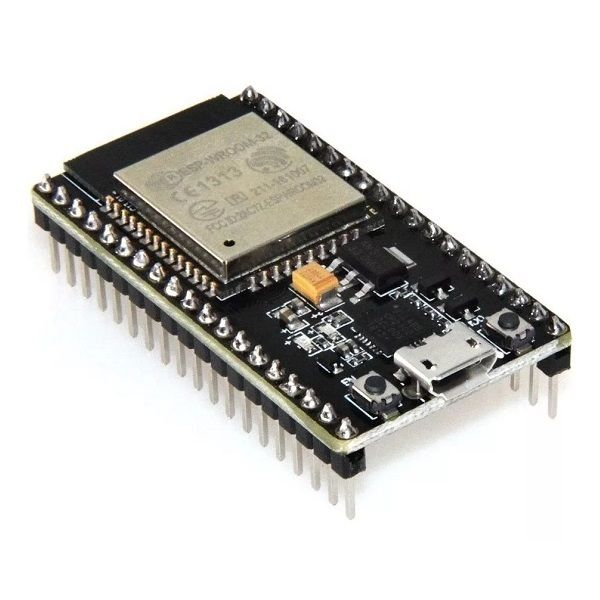
\includegraphics[width=0.2\textwidth]{ESP32.jpeg}}
  \subfigure[SG90]{
    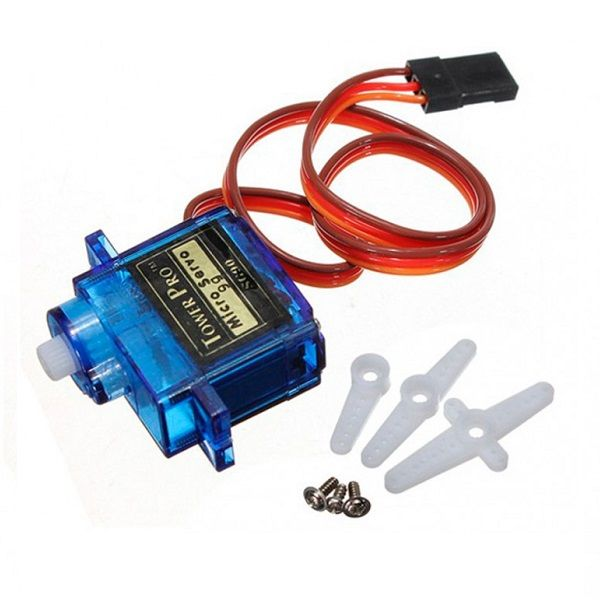
\includegraphics[width=0.2\textwidth]{SG90.jpeg}}
  \subfigure[MG946R]{
    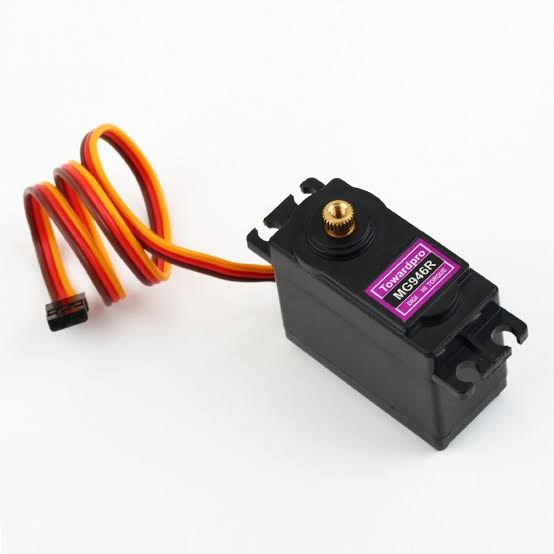
\includegraphics[width=0.2\textwidth]{MG946R.jpg}}
 \caption{Componentes principales del receptor.}
 \label{f:Receptor}
\end{figure}

En el transmisor, el movimiento de cada dedo hace girar un potenciómetro, cuya tensión lee el conversor analógico-digital (ADC) del ESP32. Además, el MPU6050 (acelerómetro y giróscopo de tres ejes) permite estimar la inclinación y la rotación de la mano. El sensor debe montarse paralelo al dorso de la mano y bien orientado, ya que un mal posicionamiento introduce un error en la medición; el firmware prevé constantes de ajuste (\textit{trim}) para compensar pequeñas desalineaciones (sección~\ref{sec:mapeo_munieca}).

\begin{figure}[H]
 \centering
  \subfigure[Potenciómetro]{
    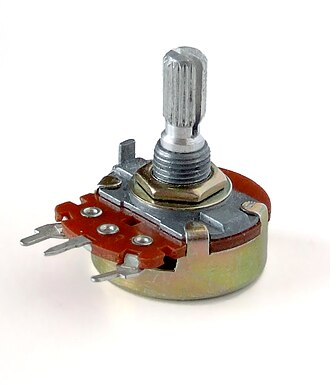
\includegraphics[width=0.2\textwidth]{Potenciometro.jpg}}
  \subfigure[MPU6050]{
    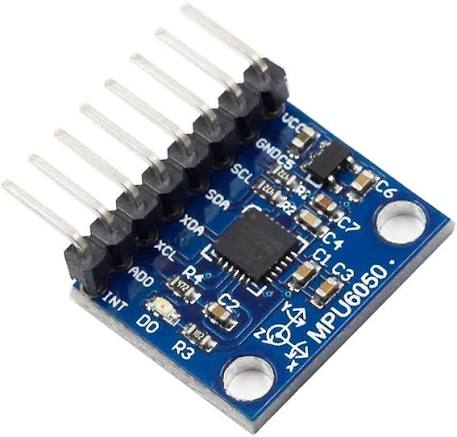
\includegraphics[width=0.2\textwidth]{MPU6050.jpg}}
 \caption{Sensores del transmisor.}
 \label{f:Transmisor}
\end{figure}

\section{Arquitectura del sistema}
\label{sec:arquitectura}

\subsection{Visión general}

La figura~\ref{fig:sistema} resume el sistema. El transmisor mide los dedos y la muñeca del operador, calcula los ángulos que deben tomar los servos y los envía por ESP-NOW 50 veces por segundo. El receptor valida cada paquete, genera una trayectoria suave hacia los ángulos recibidos y comanda los servomotores.

\begin{figure}[H]
\centering
\begin{tikzpicture}[node distance=0.6cm and 1.2cm]
  % Transmisor
  \node[bloque] (pot) {5 potenciómetros\\(dedos)};
  \node[bloque, below=of pot] (imu) {MPU6050\\(muñeca)};
  \coordinate (medio) at ($(pot)!0.5!(imu)$);
  \node[bloque, right=1.9cm of medio, fill=orange!10, minimum width=3.4cm] (tx)
       {\textbf{ESP32 Transmisor}\\ ADC sobremuestreado\\ Filtro complementario\\ Ángulos de servo\\ Empaquetado + checksum};
  \node[draw, dashed, rounded corners, inner sep=6pt, fit=(pot)(imu)(tx), label=above:{\textbf{Guante}}] {};
  % Receptor
  \node[bloque, right=1.7cm of tx, fill=green!10, minimum width=3.4cm] (rx)
       {\textbf{ESP32 Receptor}\\ Validación del paquete\\ Supervisión (failsafe)\\ Limitador de velocidad\\ Banda muerta};
  \node[bloque, right=of rx, yshift=0.8cm] (sg) {5 servos SG90\\(dedos)};
  \node[bloque, right=of rx, yshift=-0.8cm] (mg) {2 servos MG946R\\(muñeca)};
  \node[draw, dashed, rounded corners, inner sep=6pt, fit=(rx)(sg)(mg), label=above:{\textbf{Mano robótica}}] {};
  % Flechas
  \draw[flecha] (pot) -- (tx);
  \draw[flecha] (imu) -- (tx);
  \draw[flecha, very thick, blue!60!black] (tx) -- node[above, font=\footnotesize, align=center]{ESP-NOW\\2,4 GHz} node[below, font=\footnotesize, align=center]{19 bytes\\50 Hz} (rx);
  \draw[flecha] (rx) -- node[above, font=\footnotesize]{PWM} (sg);
  \draw[flecha] (rx) -- node[below, font=\footnotesize]{PWM} (mg);
\end{tikzpicture}
\caption{Diagrama en bloques del sistema.}
\label{fig:sistema}
\end{figure}

Una decisión de diseño atraviesa todo el firmware: \textbf{el transmisor envía ángulos de servo ya calculados} (por ejemplo, \SIrange{25}{90}{\degree} para los dedos), no lecturas crudas de los sensores. De este modo, toda la calibración propia del operador reside en el guante y el receptor sólo se ocupa de mover los motores de forma segura. Si cambia el operador, se recalibra el guante sin modificar la mano.

\subsection{Organización del firmware en tiempo real}

\pendiente{Revisar en detalle el diagrama tipo clases del firmware (\texttt{informe/\allowbreak borradores/\allowbreak diagrama\_firmware.tex}) y anexarlo al informe.}

Ambos firmwares están escritos en C++ sobre el núcleo Arduino para ESP32, que a su vez corre sobre el sistema operativo de tiempo real FreeRTOS. El ESP32 tiene dos núcleos: la pila Wi-Fi (y por lo tanto ESP-NOW) se ejecuta por defecto en el núcleo 0, por lo que las tareas de control de este proyecto se fijaron al núcleo 1 con \texttt{xTaskCreatePinnedToCore()}. La tabla~\ref{tab:tareas} resume las tareas de cada nodo.

\begin{table}[H]
\centering
\begin{tabularx}{\textwidth}{l l c c X}
\toprule
\textbf{Nodo} & \textbf{Tarea} & \textbf{Núcleo} & \textbf{Prioridad} & \textbf{Función} \\
\midrule
Transmisor & \texttt{tareaTransmision} & 1 & 2 & Ciclo periódico de \SI{20}{\milli\second}: IMU, dedos, empaquetado y envío \\
Transmisor & \texttt{loop()} & 1 & 1 & Atiende el puerto serie (comando de calibración) \\
Receptor & Callback ESP-NOW & 0 & --- & Valida el paquete y lo deposita en la cola (corre en la tarea Wi-Fi) \\
Receptor & \texttt{tareaControlActuadores} & 1 & 3 & Supervisión del enlace, trayectoria y escritura de los servos \\
\bottomrule
\end{tabularx}
\caption{Tareas FreeRTOS de cada nodo.}
\label{tab:tareas}
\end{table}

\subsection{Protocolo de comunicación}
\label{sec:protocolo}

Ambos nodos comparten el archivo \texttt{ProtocoloBrazo.h}, que define la estructura del paquete y las funciones de verificación. Como el entorno de Arduino sólo compila archivos que están dentro de la carpeta de cada programa, existen dos copias idénticas del archivo, una por nodo, que deben mantenerse iguales.

\begin{lstlisting}[caption={Estructura del paquete (\texttt{ProtocoloBrazo.h}).}, label={cod:paquete}]
#pragma pack(push, 1)
struct MensajeBrazo {
    uint16_t magicHeader;        // 0xAA55
    uint8_t  secuencia;          // 0..255, incremental
    uint16_t anguloDedos[5];     // 25..90°
    int16_t  muniecaVertical;    // 25..90°
    int16_t  muniecaRotacional;  // 0..180°
    uint16_t checksum;           // Fletcher-16
};
#pragma pack(pop)
\end{lstlisting}

La directiva \texttt{\#pragma pack(push, 1)} evita que el compilador agregue bytes de relleno (\textit{padding}) para alinear los campos de 16 bits. Así, la estructura ocupa exactamente 19 bytes y tiene la misma disposición en memoria en ambos ESP32, lo que permite enviarla tal cual y reinterpretarla del otro lado sin serializar campo por campo. La tabla~\ref{tab:paquete} detalla la trama, muy por debajo del máximo de 250 bytes por paquete que admite ESP-NOW \cite{espnow_idf}.

\begin{table}[H]
\centering
\begin{tabular}{c l c l}
\toprule
\textbf{Bytes} & \textbf{Campo} & \textbf{Tamaño} & \textbf{Contenido} \\
\midrule
0--1   & \texttt{magicHeader}       & 2 & Firma fija \texttt{0xAA55} \\
2      & \texttt{secuencia}         & 1 & Contador que vuelve a 0 después de 255 \\
3--12  & \texttt{anguloDedos[0..4]} & 10 & Pulgar, índice, medio, anular y meñique \\
13--14 & \texttt{muniecaVertical}   & 2 & Ángulo del servo de muñeca vertical \\
15--16 & \texttt{muniecaRotacional} & 2 & Ángulo del servo de rotación \\
17--18 & \texttt{checksum}          & 2 & Fletcher-16 de los bytes 0 a 16 \\
\midrule
       & \textbf{Total}             & \textbf{19} & \\
\bottomrule
\end{tabular}
\caption{Formato de la trama.}
\label{tab:paquete}
\end{table}

\subsubsection{Verificación de integridad}

El receptor acepta un paquete sólo si cumple tres condiciones: su longitud es de 19 bytes, comienza con la firma \texttt{0xAA55} y su suma de verificación coincide. La suma de verificación es el algoritmo de Fletcher \cite{fletcher1982}, calculado sobre los $N = 17$ bytes $b_i$ previos al campo \texttt{checksum}:
\begin{equation}
s_1^{(i)} = \left(s_1^{(i-1)} + b_i\right) \bmod 255, \qquad
s_2^{(i)} = \left(s_2^{(i-1)} + s_1^{(i)}\right) \bmod 255, \qquad
\text{checksum} = 256\, s_2^{(N)} + s_1^{(N)}
\end{equation}
con $s_1^{(0)} = s_2^{(0)} = 0$. La suma $s_1$ acumula el valor de los bytes y $s_2$ acumula las sumas parciales, por lo que depende también de la \emph{posición} de cada byte: a diferencia de una suma simple, detecta bytes intercambiados. También detecta cualquier error de un único bit. Se eligió frente a un CRC por su simplicidad (sólo sumas, sin tablas ni polinomios); la capa MAC de Wi-Fi (IEEE 802.11) ya incorpora su propio CRC-32, por lo que este control funciona como una segunda barrera a nivel de aplicación, por ejemplo frente a paquetes de otro dispositivo ESP-NOW cercano.

El número de \texttt{secuencia} se incrementa en cada envío y permite identificar paquetes perdidos al analizar la telemetría.

\section{Transmisor}
\label{sec:transmisor}

\subsection{Diseño mecánico del guante}

El guante se diseñó en Solid Edge (ver sección~\ref{sec:disenio_receptor}) y se imprimió en 3D. La figura~\ref{fig:guante} muestra el conjunto. Sobre el dorso de la mano se apoya una base que aloja los cinco potenciómetros; cada dedo del operador se vincula a su potenciómetro mediante una tanza que recorre el dorso del dedo, guiada por dedales colocados en las falanges. Sobre la muñeca se ubica el soporte del ESP32.

\begin{figure}[H]
 \centering
  \subfigure[Conjunto]{
    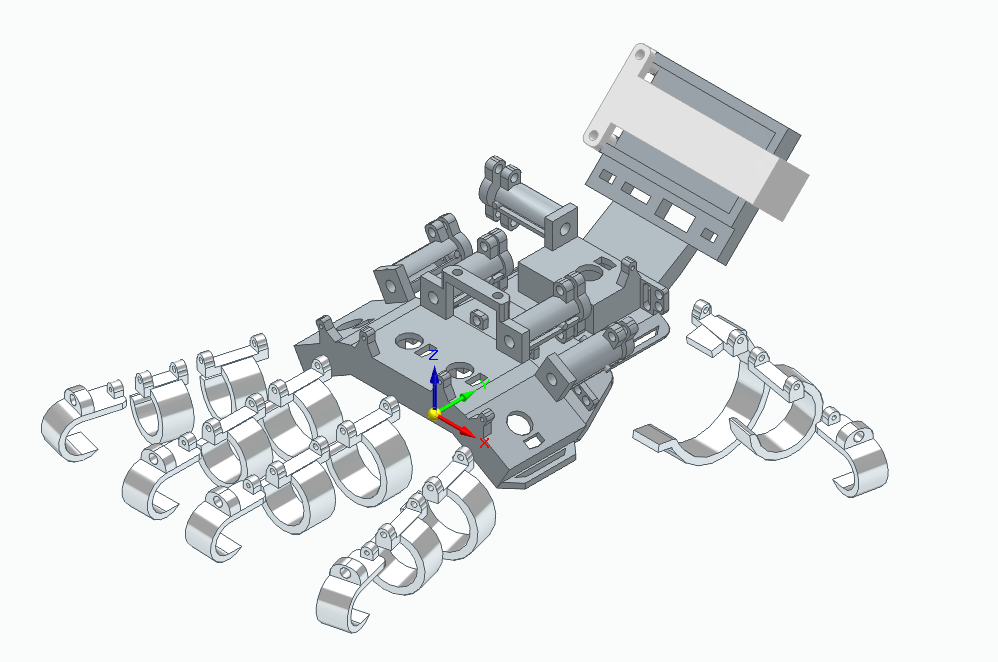
\includegraphics[width=0.48\textwidth]{Transmisor/GuanteCompleto.png}}
  \subfigure[Base dorsal]{
    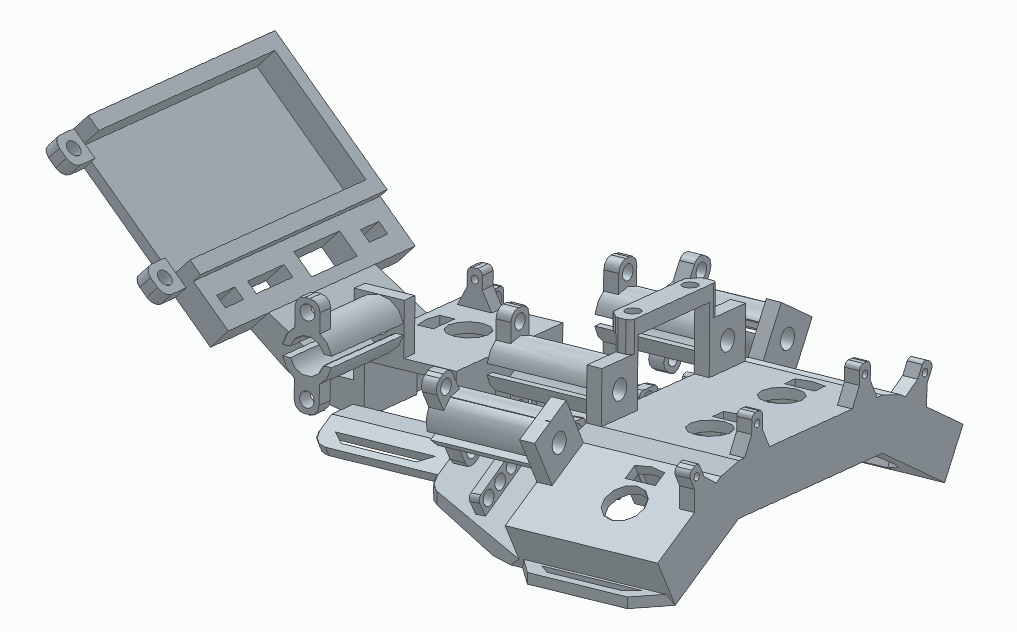
\includegraphics[width=0.45\textwidth]{Transmisor/Dorsal.png}}
 \caption{Diseño del guante transmisor.}
 \label{fig:guante}
\end{figure}

\begin{figure}[H]
 \centering
  \subfigure[Dedal de la punta]{
    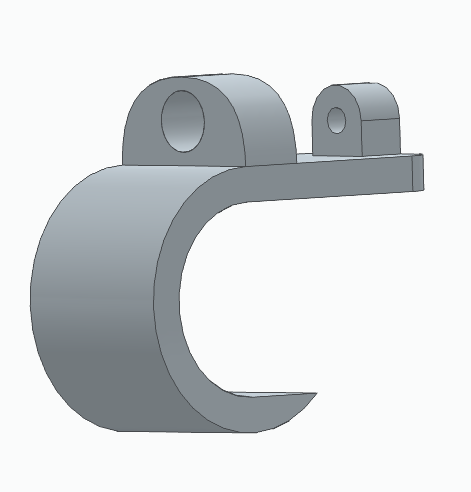
\includegraphics[width=0.18\textwidth]{Transmisor/Dedal_1.png}}
  \subfigure[Dedal guía de falange]{
    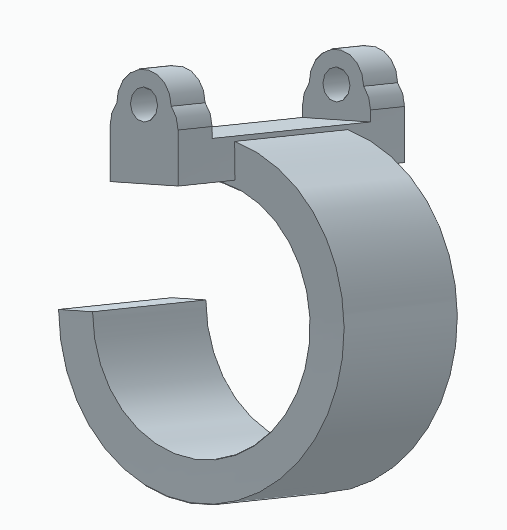
\includegraphics[width=0.18\textwidth]{Transmisor/Dedal_2.png}}
  \subfigure[Dedal del pulgar]{
    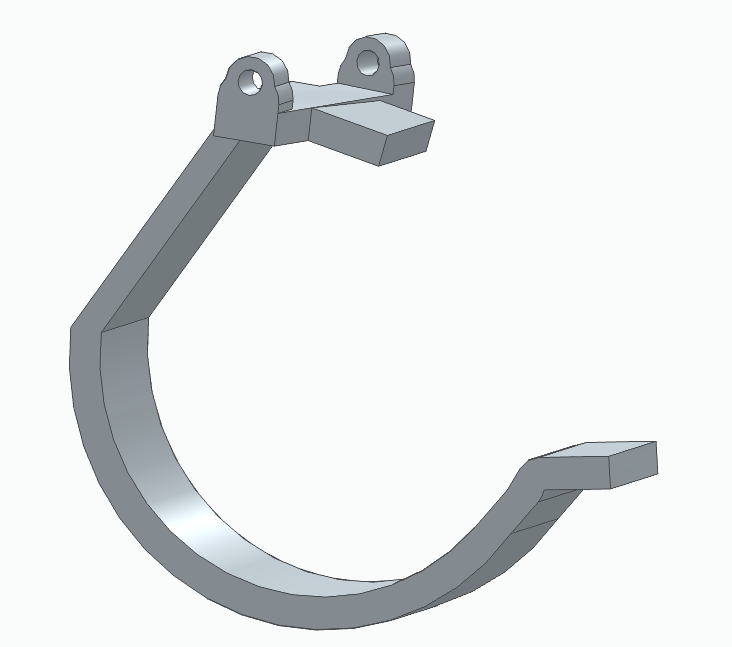
\includegraphics[width=0.18\textwidth]{Transmisor/Dedal_3_Pulgar.png}}
  \subfigure[Resortera]{
    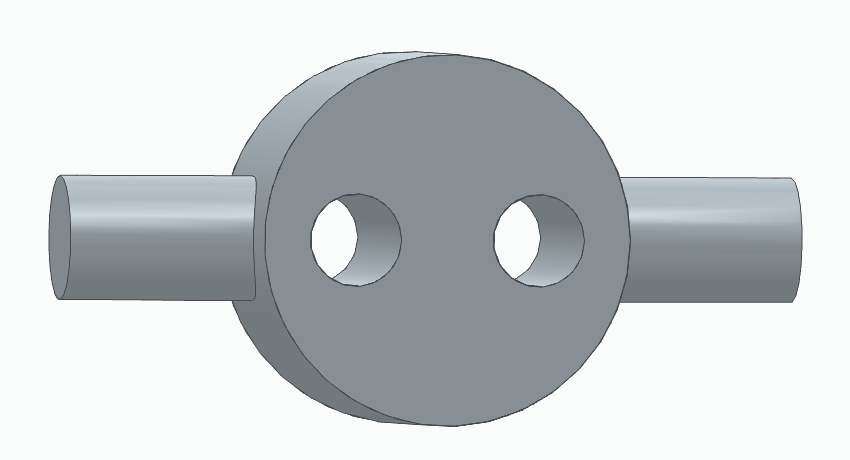
\includegraphics[width=0.2\textwidth]{Transmisor/Resortera.png}}
  \subfigure[Tapa del potenciómetro]{
    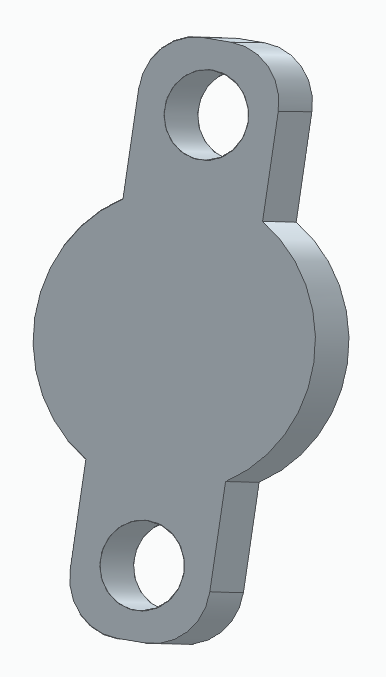
\includegraphics[width=0.1\textwidth]{Transmisor/Tapa_Pote.png}}
  \subfigure[Agarre del ESP32]{
    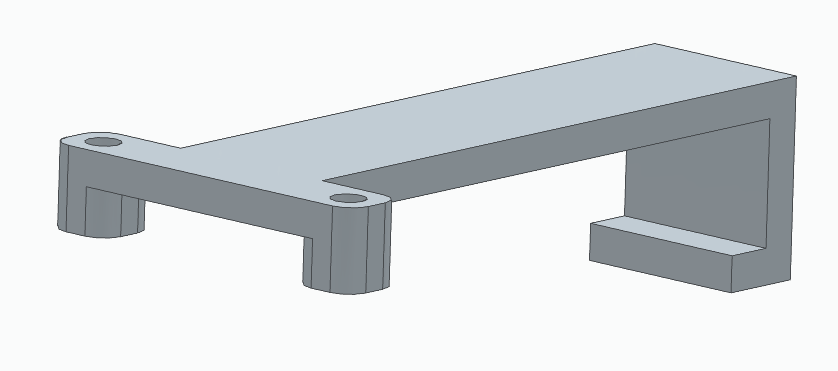
\includegraphics[width=0.25\textwidth]{Transmisor/Agarre_ESP.png}}
  \subfigure[Palanca del potenciómetro]{
    \parbox{0.2\textwidth}{\centering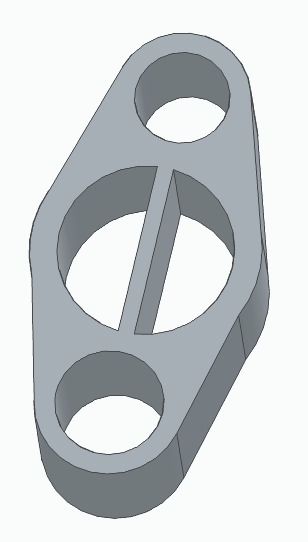
\includegraphics[width=0.08\textwidth]{Transmisor/Palanca_Pote.jpg}}}
 \caption{Piezas del guante.}
 \label{fig:piezas_guante}
\end{figure}

El movimiento de cada dedo llega a su potenciómetro a través de una tanza, siguiendo este recorrido:

\begin{enumerate}
    \item \textbf{Dedal de la punta:} un extremo de la tanza está atado a este dedal, colocado en la falange distal. Su tamaño varía ligeramente según el dedo.
    \item \textbf{Dedales guía:} la tanza recorre la parte superior del dedo sujeta a un dedal en cada falange, que la mantiene cerca del dedo. Sus medidas también dependen del dedo. En el pulgar, uno de estos dedales se ubica sobre el metacarpiano, una zona más gruesa y de forma distinta, por lo que es una pieza propia hecha más a medida.
    \item \textbf{Palanca del potenciómetro:} ya sobre el dorso de la mano, la tanza se une a una pequeña palanca impresa en 3D montada en el eje del potenciómetro (figura~\ref{fig:piezas_guante}g). Al flexionar el dedo, la tanza tira de la palanca y hace girar el eje.
    \item \textbf{Resorte y resortera:} desde la palanca, la tanza continúa hasta un pequeño tubo horizontal que contiene un resorte (hay cinco tubos sobre la base dorsal, uno por dedo), pasa por dentro del resorte y termina atada a la resortera. Al cerrar el dedo, la tanza arrastra la resortera y comprime el resorte.
    \item \textbf{Retorno:} al abrir el dedo, el resorte se descomprime, empuja la resortera hacia su posición natural y mantiene la tanza tensa, de modo que el eje del potenciómetro vuelve a la posición de reposo. El fin de ese recorrido lo marca la pieza llamada tapa del potenciómetro, que es en realidad la tapa trasera del tubo del resorte.
\end{enumerate}

El resorte cumple dos funciones: devuelve el potenciómetro a su posición cuando el dedo se abre y mantiene la tanza siempre tensa, lo que reduce la holgura al inicio del movimiento. El agarre del ESP32 fija la placa sobre la muñeca.

Al flexionar el dedo, sus tres falanges producen un desplazamiento del elemento de transmisión que, aproximadamente, es la suma de las contribuciones de cada articulación:
\begin{equation}
\Delta x \approx r_1\,\Delta\theta_1 + r_2\,\Delta\theta_2 + r_3\,\Delta\theta_3 ,
\end{equation}
donde $r_j$ es la distancia efectiva entre el elemento de transmisión y el eje de la articulación $j$. Ese desplazamiento tira de la palanca del potenciómetro, de largo $R$, y hace girar su eje un ángulo $\Delta\phi \approx \Delta x / R$. La relación es sólo aproximada: vale mientras la tanza tire casi perpendicular a la palanca, y deja de ser lineal a medida que la palanca gira. Como los radios $r_j$ dependen de la mano de cada operador y del ajuste del guante, la relación entre la flexión del dedo y la lectura del ADC no es la misma para todos los usuarios ni para todos los dedos. Además aparecen holguras al inicio del recorrido e histéresis por rozamiento. Por este motivo el firmware no usa una relación fija, sino una calibración de dos puntos por dedo (sección~\ref{sec:calibracion_dedos}). Esa calibración corrige la escala y el desplazamiento de cada dedo, pero no la falta de linealidad del mecanismo, que se traslada al ángulo del servo.

\subsection{Conexionado}

La tabla~\ref{tab:pines_tx} resume las conexiones del transmisor.

\begin{table}[H]
\centering
\begin{tabular}{l c l}
\toprule
\textbf{Señal} & \textbf{GPIO} & \textbf{Observación} \\
\midrule
Potenciómetro pulgar   & 39 & ADC1 (\texttt{SENSOR\_VN}) \\
Potenciómetro índice   & 34 & ADC1 \\
Potenciómetro medio    & 35 & ADC1 \\
Potenciómetro anular   & 32 & ADC1 \\
Potenciómetro meñique  & 33 & ADC1 \\
MPU6050 SDA            & 21 & Bus I\textsuperscript{2}C a \SI{400}{\kilo\hertz} \\
MPU6050 SCL            & 22 & Bus I\textsuperscript{2}C a \SI{400}{\kilo\hertz} \\
\bottomrule
\end{tabular}
\caption{Asignación de pines del transmisor.}
\label{tab:pines_tx}
\end{table}

Todos los potenciómetros se conectan a pines del ADC1. El ESP32 tiene dos conversores, pero el ADC2 no puede utilizarse mientras la radio Wi-Fi está activa \cite{esp32_adc}, y ESP-NOW requiere la radio encendida.

La figura~\ref{fig:conexionado_tx} muestra el conexionado completo del guante. Los cinco potenciómetros, de \SI{10}{\kilo\ohm} lineales, se conectan entre \SI{3.3}{\volt} y GND, de modo que la tensión de cada cursor nunca supera el rango de entrada del ADC. El módulo MPU6050 (GY-521) se alimenta del pin de \SI{5}{\volt} del ESP32, ya que incluye su propio regulador de \SI{3.3}{\volt}.

El guante se alimenta por el conector USB del ESP32 desde la computadora, la misma conexión que se usa para la calibración y la telemetría; el regulador de la placa genera los \SI{3.3}{\volt}. Un \textit{powerbank} de \SI{5}{\volt} queda como alternativa si se necesitara independizarlo de la computadora.

\begin{figure}[H]
    \centering
    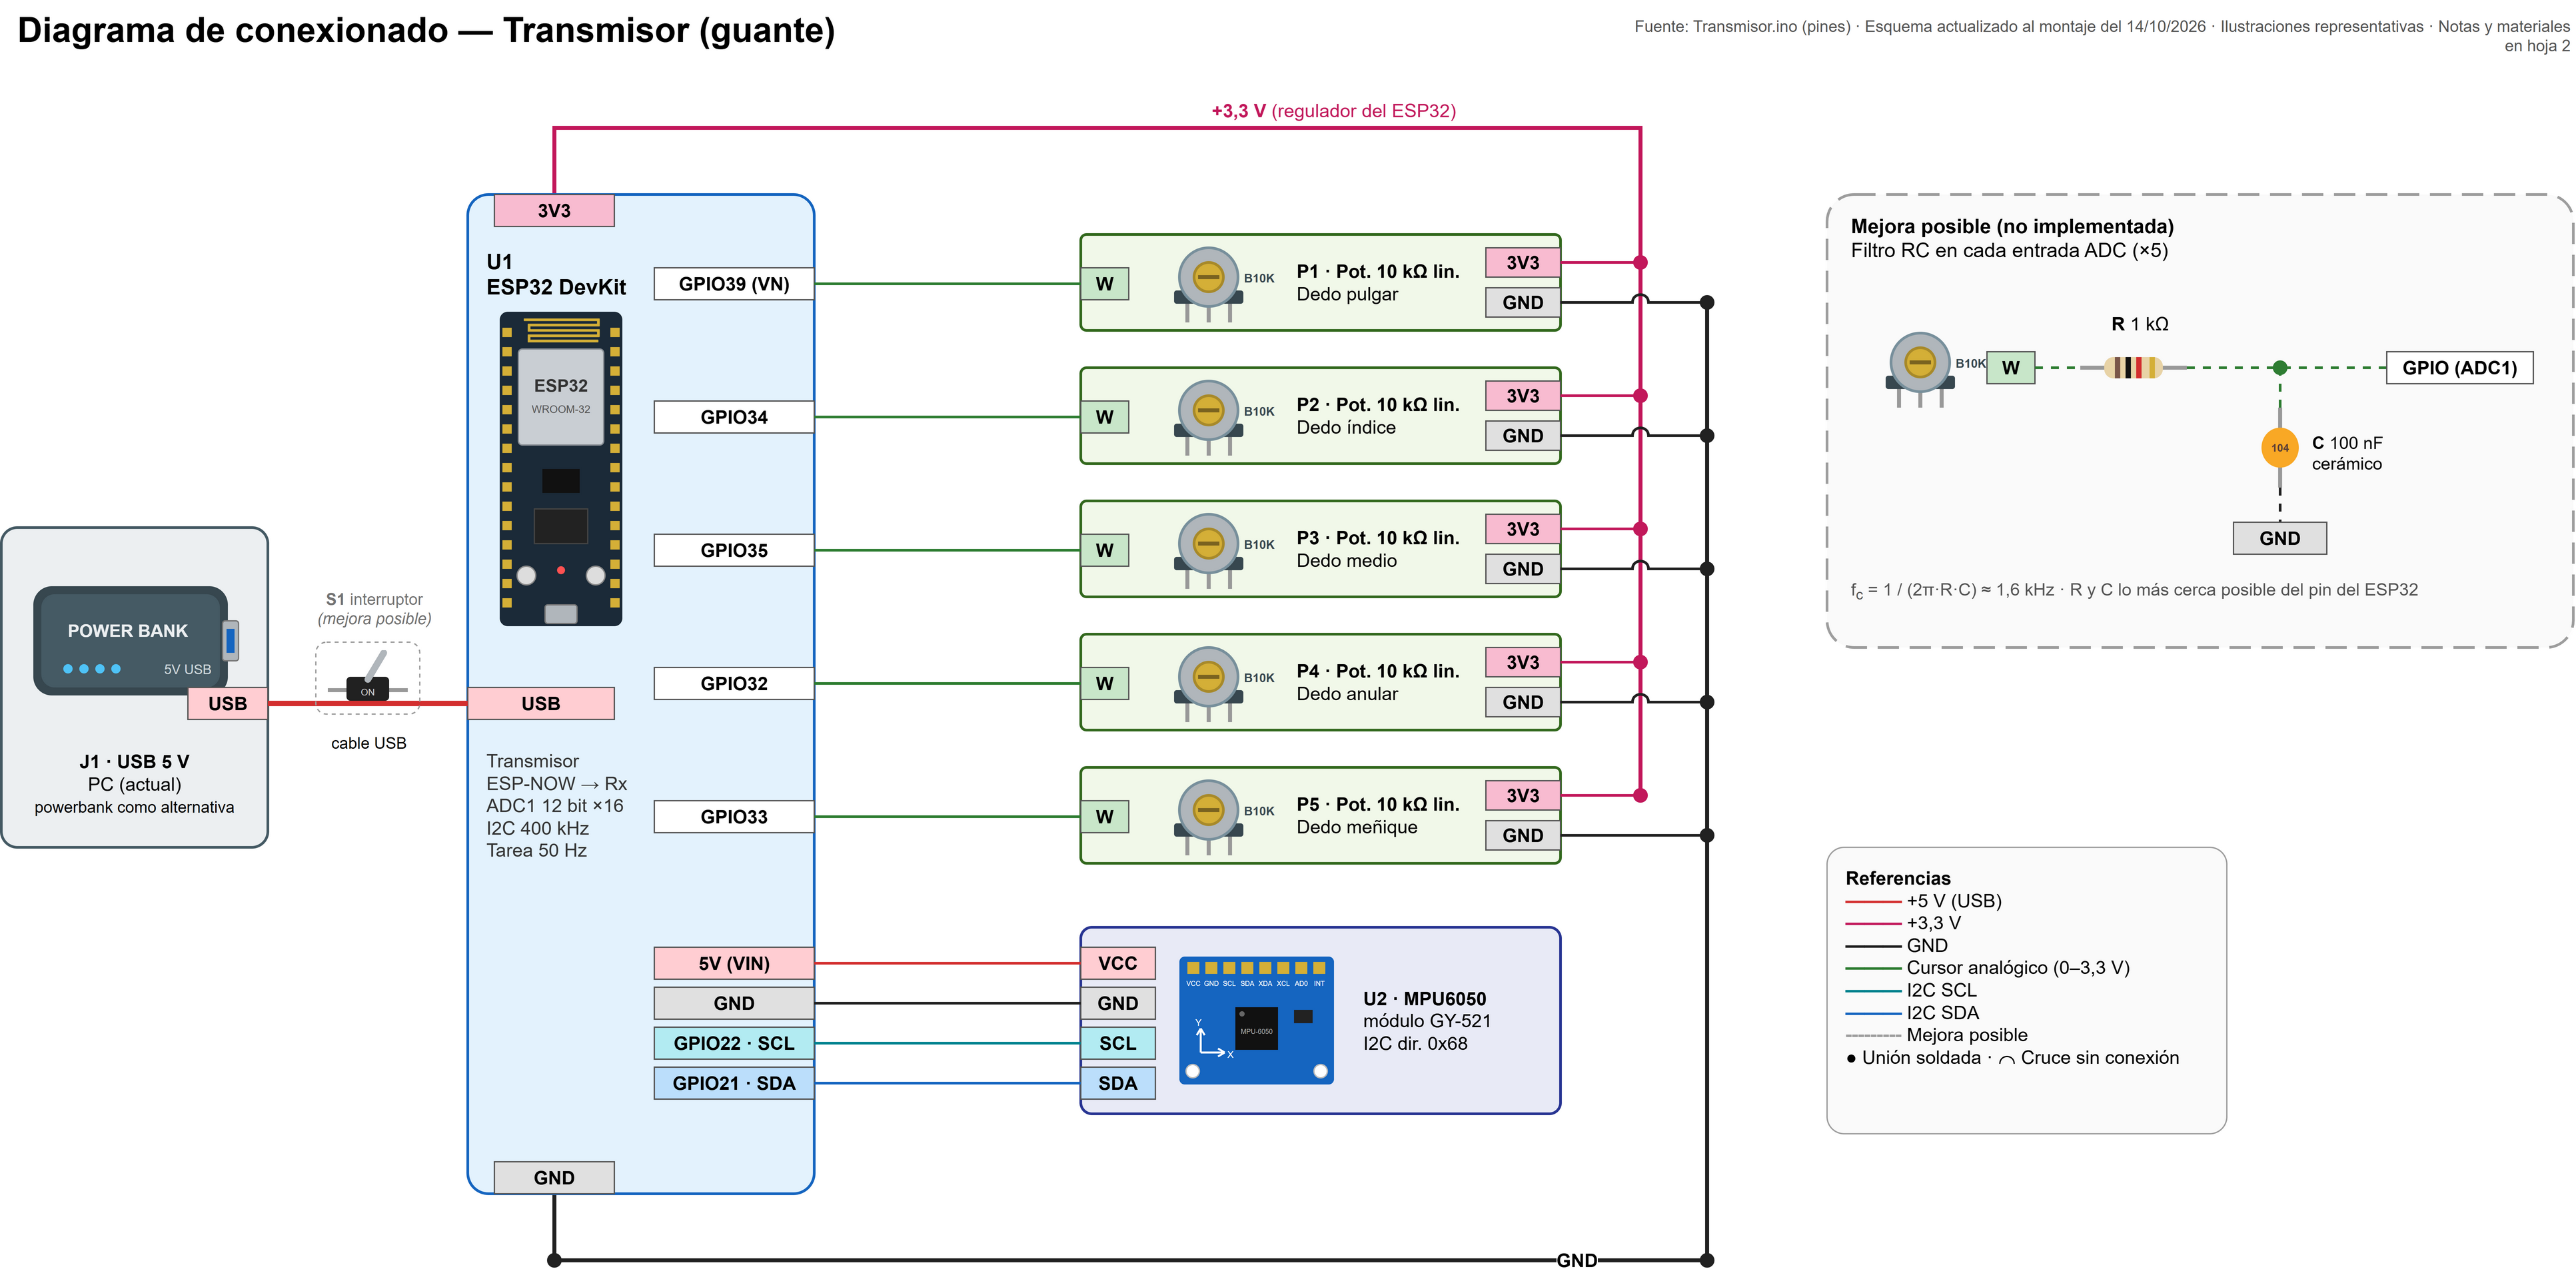
\includegraphics[width=\textwidth]{Conexionado_Transmisor_Diagrama.png}
    \caption{Diagrama de conexionado del transmisor. El filtro RC de la derecha es una mejora posible que no se implementó.}
    \label{fig:conexionado_tx}
\end{figure}

\subsection{Fundamentos de la unidad de medición inercial}

\begin{itemize}
    \item \textbf{Giróscopo:}

    Es un dispositivo que permite medir la rotación de un mecanismo. Los giróscopos de los sensores MEMS como el MPU6050 son giróscopos vibratorios de efecto Coriolis (CVG, por sus siglas en inglés). Su principio de funcionamiento es que un objeto vibratorio tiende a seguir vibrando en el mismo plano aunque su soporte rote; el efecto Coriolis hace que el objeto ejerza una fuerza sobre el soporte, y midiendo esa fuerza se determina la rotación a la que está sometido el sensor.

    \begin{figure}[H]
    \begin{center}
 		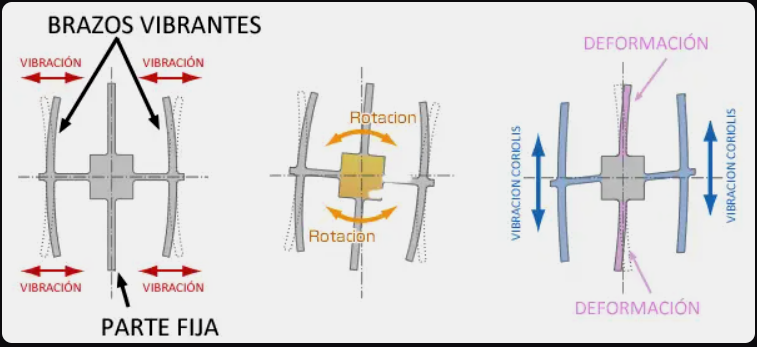
\includegraphics[scale=0.6]{Giroscopio.png}
 		\captionof{figure}{Giróscopo.}
        \label{fig:giroscopio}
    \end{center}
    \end{figure}

    Una consecuencia de emplear la fuerza de Coriolis es que estos giróscopos no registran el ángulo girado sino la \emph{velocidad angular}. Para obtener el ángulo es necesario integrar la medición respecto del tiempo. Los giróscopos responden rápido y con buena precisión en tiempos cortos, y siguen bien los cambios bruscos; pero, al integrar, cualquier error pequeño y constante en la velocidad (\textit{bias}) se acumula y el ángulo deriva (\textit{drift}). Con un \textit{bias} $b$, el error del ángulo crece linealmente con el tiempo:
    \begin{equation}
    \theta(t) = \int_0^t \omega\,dt \quad\Rightarrow\quad \theta_{\text{error}}(t) = b\,t.
    \end{equation}
    Por ejemplo, con $b = \SI{0.01}{\radian\per\second} \approx \SI{0.57}{\degree\per\second}$, que es el orden de \textit{bias} esperado para este sensor según el plan de pruebas (no un valor medido), el ángulo se desvía unos \SI{34}{\degree} en un minuto. Por eso el \textit{bias} se mide al encender y se resta (sección~\ref{sec:fusion}), y el error residual lo corrige el acelerómetro.

    \item \textbf{Acelerómetro:}

    Es un dispositivo que mide la aceleración a la que está sometido. Puede pensarse como un cuerpo sólido en cuyo interior hay una masa suspendida por resortes.

    \begin{figure}[H]
    \begin{center}
 		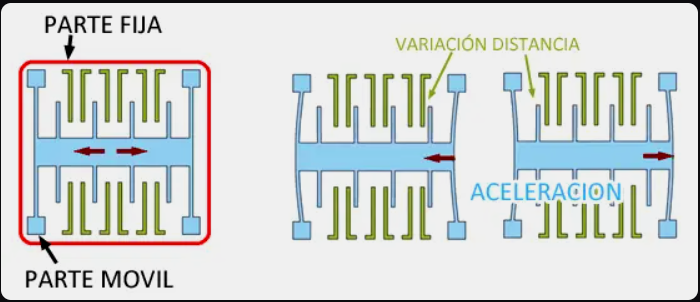
\includegraphics[scale=0.6]{Acelerometro.png}
 		\captionof{figure}{Acelerómetro.}
        \label{fig:acelerometro}
    \end{center}
    \end{figure}

    Al aplicar una aceleración al conjunto, la masa suspendida ejerce una fuerza sobre los resortes y su posición relativa dentro del sensor varía. Ese desplazamiento es proporcional a la aceleración y puede medirse. El sensor también registra la gravedad terrestre, de aproximadamente \SI{9.81}{\meter\per\second\squared}; con el sensor en reposo, la dirección de la gravedad respecto de los ejes del sensor permite determinar su orientación (figura~\ref{fig:orientacion}). La limitación es que, cuando la mano acelera, el sensor mide gravedad más movimiento y el ángulo calculado se contamina.

    \begin{figure}[H]
    \begin{center}
 		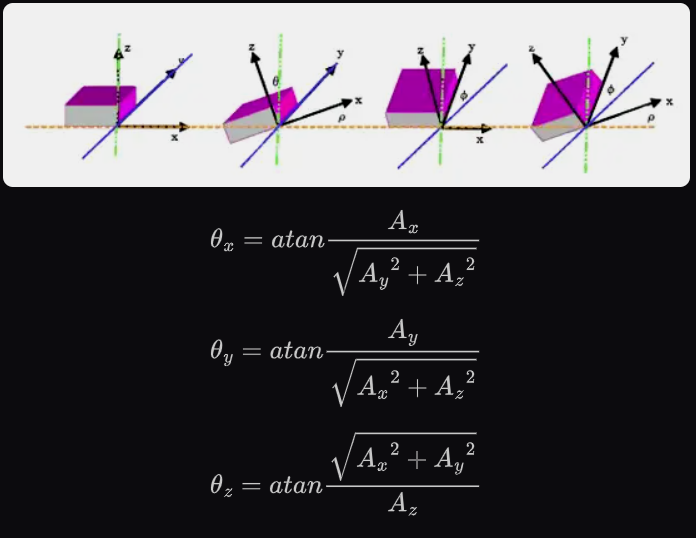
\includegraphics[scale=0.5]{Acelerometro_Calculo.png}
 		\captionof{figure}{Orientación a partir de la gravedad.}
        \label{fig:orientacion}
    \end{center}
    \end{figure}
\end{itemize}

El MPU6050 integra un acelerómetro y un giróscopo de tres ejes cada uno; es una unidad de medición inercial (IMU) de 6 grados de libertad. Cada eje entrega un valor de 16 bits, y el ESP32 lee los 14 bytes de una medición completa por I\textsuperscript{2}C. Con los rangos configurados en este proyecto, las sensibilidades de la hoja de datos son 65,5~LSB/(\si{\degree\per\second}) para el giróscopo ($\pm\SI{500}{\degree\per\second}$) y 16384~LSB/$g$ para el acelerómetro ($\pm 2\,g$). La orientación se describe con los ángulos de Tait-Bryan: rotaciones en torno al eje X (\textit{roll}), al eje Y (\textit{pitch}) y al eje Z (\textit{yaw}) (figura~\ref{fig:rotaciones}). En este proyecto se utilizan el \textit{pitch}, que corresponde a la flexión de la muñeca hacia arriba y abajo, y el \textit{roll}, que corresponde a la rotación de la mano. El \textit{yaw} no puede obtenerse del acelerómetro (la gravedad no cambia al girar alrededor del eje vertical) y no se utiliza.

\begin{figure}[H]
    \begin{center}
 		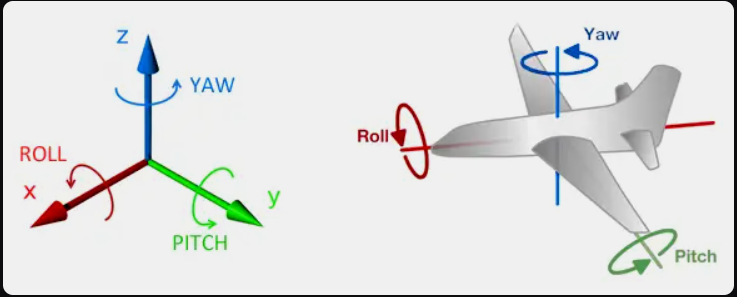
\includegraphics[scale=0.5]{Rotaciones.png}
 		\captionof{figure}{Rotaciones de Tait-Bryan.}
        \label{fig:rotaciones}
    \end{center}
\end{figure}

Las dos fuentes de información son complementarias: el giróscopo es confiable a corto plazo y el acelerómetro a largo plazo. Para aprovechar ambas se las combina con un filtro de fusión, que se describe en la sección~\ref{sec:fusion}.

\subsection{Firmware del transmisor}

\subsubsection{Inicialización}

Al encender, la función \texttt{setup()} ejecuta los siguientes pasos:

\begin{enumerate}
    \item Configura el ADC con 12 bits de resolución (0 a 4095) y atenuación de \SI{11}{\deci\bel}, que amplía el rango de entrada a aproximadamente 0--\SI{3.3}{\volt}.
    \item Carga la calibración de los dedos desde la memoria no volátil (sección~\ref{sec:calibracion_dedos}).
    \item Libera el bus I\textsuperscript{2}C (ver más abajo) e inicia la comunicación con el MPU6050 a \SI{400}{\kilo\hertz}, con hasta cinco intentos.
    \item Configura el MPU6050: acelerómetro en $\pm 2\,g$ (máxima resolución; la mano no supera esa aceleración en uso normal), giróscopo en $\pm\SI{500}{\degree\per\second}$ y filtro pasa-bajos interno en \SI{44}{\hertz}. Luego calibra el sensor en reposo (sección~\ref{sec:fusion}).
    \item Inicia la radio en modo estación, desactiva el ahorro de energía de la radio (\texttt{WiFi.setSleep(false)}), que agrega latencia, y registra al receptor como destino (\textit{peer}) de ESP-NOW mediante su dirección MAC, sin cifrado.
    \item Crea la tarea periódica \texttt{tareaTransmision} en el núcleo 1.
\end{enumerate}

\paragraph{Recuperación del bus I\textsuperscript{2}C.} Si el ESP32 se reinicia en medio de una lectura, el MPU6050 puede quedar a mitad de la transmisión de un byte, manteniendo la línea SDA en nivel bajo. El bus queda bloqueado y la inicialización falla aunque el sensor funcione. Para evitarlo, antes de iniciar el bus se generan manualmente nueve pulsos de reloj en SCL, suficientes para que el esclavo termine de enviar el byte pendiente y libere SDA, seguidos de una condición de STOP. Es el procedimiento de \textit{bus clear} de la especificación de I\textsuperscript{2}C \cite{nxp_i2c}.

\subsubsection{Ciclo periódico}

La tarea \texttt{tareaTransmision} se ejecuta cada \SI{20}{\milli\second} (\SI{50}{\hertz}) mediante \texttt{vTaskDelayUntil()}, que mide el período desde el despertar anterior y no desde el final del trabajo \cite{freertos}. A diferencia de un \texttt{delay(20)} al final del bucle, el período no se alarga con el tiempo de cómputo: la tarea despierta en instantes absolutos (0, 20, \SI{40}{\milli\second}, etc.). Si un ciclo excediera los \SI{20}{\milli\second}, \texttt{vTaskDelayUntil()} no esperaría y el ciclo siguiente arrancaría enseguida, de modo que la grilla de tiempos se mantiene y el atraso no se acumula. La figura~\ref{fig:ciclo_tx} muestra el orden de cada ciclo.

\begin{figure}[H]
\centering
\begin{tikzpicture}[node distance=0.45cm, every node/.style={font=\small}]
  \node[bloque, fill=gray!10] (t) {Despertar (cada \SI{20}{\milli\second})};
  \node[bloque, below=of t] (imu) {Leer MPU6050 y aplicar el filtro complementario\\Calcular ángulos de servo de la muñeca};
  \node[draw, diamond, aspect=2.5, below=of imu, inner sep=1pt, fill=yellow!10] (cal) {¿Calibrando?};
  \node[bloque, below=of cal] (ded) {Leer los 5 potenciómetros (16 muestras c/u)\\Convertir a ángulo con la calibración};
  \node[bloque, below=of ded] (env) {Armar paquete, secuencia y checksum\\Enviar por ESP-NOW};
  \node[bloque, below=of env] (tel) {Telemetría serie (1 de cada 10 ciclos)};
  \draw[flecha] (t) -- (imu);
  \draw[flecha] (imu) -- (cal);
  \draw[flecha] (cal) -- node[right]{No} (ded);
  \draw[flecha] (ded) -- (env);
  \draw[flecha] (env) -- (tel);
  \draw[flecha] (cal.east) -- node[above]{Sí} ++(2.8,0) |- (t.east);
  \draw[flecha] (tel.west) -- ++(-3.8,0) |- (t.west);
\end{tikzpicture}
\caption{Ciclo de la tarea de transmisión.}
\label{fig:ciclo_tx}
\end{figure}

\subsubsection{Sensado de los dedos}

\paragraph{Sobremuestreo.} El ADC del ESP32 presenta ruido de varias cuentas. Para reducirlo, cada lectura es el promedio de 16 conversiones separadas por \SI{50}{\micro\second}. Si el ruido es aleatorio e independiente entre muestras, el promedio de $N$ muestras reduce su desviación estándar en un factor $\sqrt{N}$:
\begin{equation}
\sigma_{\bar{x}} = \frac{\sigma}{\sqrt{N}} = \frac{\sigma}{4} \quad (N = 16).
\end{equation}
El promedio no corrige la alinealidad propia del ADC; ésta queda absorbida en parte por la calibración de dos puntos. Leer los cinco dedos de esta forma insume del orden de \SI{5}{\milli\second}, que entra con holgura en el período de \SI{20}{\milli\second}.

\paragraph{Calibración de dos puntos.}
\label{sec:calibracion_dedos}
Cada dedo tiene dos valores de calibración: la lectura con la mano abierta, $ADC_{\min}$, y con el puño cerrado, $ADC_{\max}$. Se almacenan en la memoria flash no volátil (NVS) del ESP32 mediante la librería \texttt{Preferences}, por lo que se conservan al apagar y al reprogramar el firmware. Si nunca se calibró, se usan 1200 y 3200 por defecto. La lectura se convierte a un ángulo lógico del dedo, entre \SI{25}{\degree} (extendido) y \SI{90}{\degree} (flexionado), por interpolación lineal y saturación:
\begin{equation}
\theta_{\text{dedo}} = \operatorname{sat}_{[25,\,90]}\!\left( 25 + \left(ADC - ADC_{\min}\right)\frac{90 - 25}{ADC_{\max} - ADC_{\min}} \right).
\end{equation}
La saturación evita que, si el operador abre o cierra la mano más que durante la calibración, el ángulo salga del rango mecánico de la mano robótica. Como la fórmula admite $ADC_{\max} < ADC_{\min}$, un potenciómetro montado al revés también funciona sin cambios en el código.

\paragraph{Procedimiento de calibración.} Se inicia enviando el carácter \texttt{c} por el monitor serie. El firmware pide abrir la mano y presionar ENTER (registra los mínimos promediando 32 muestras), luego cerrar el puño y presionar ENTER (registra los máximos) y finalmente guarda los diez valores en la NVS. Durante la calibración la tarea de transmisión deja de leer los dedos, de transmitir y de imprimir telemetría; sólo sigue leyendo la IMU para no perder el estado del filtro de la muñeca. En consecuencia, el receptor deja de recibir paquetes, entra en su modo de seguridad y lleva la mano a la posición de reposo (sección~\ref{sec:fsm}); al terminar la calibración el envío se reanuda y la mano vuelve a seguir al guante sin intervención. Este comportamiento se agregó en la versión 2.3.0 y se verificó en hardware.

\subsubsection{Estimación de la orientación de la muñeca}
\label{sec:fusion}

\paragraph{Calibración en reposo.} Al encender, con la mano quieta, se toman 500 lecturas (aproximadamente \SI{1.5}{\second}) y se calculan:
\begin{itemize}
    \item el \textit{bias} de los ejes X e Y del giróscopo, es decir, el valor que miden estando quietos, que luego se resta en cada lectura; y
    \item los ángulos iniciales de \textit{pitch} y \textit{roll} según el acelerómetro, para que el filtro arranque en la orientación real y no en \SI{0}{\degree}.
\end{itemize}

\paragraph{Ángulos por acelerómetro.} Con el sensor en reposo, la inclinación se obtiene de las componentes de la gravedad \cite{pedley_an3461}:
\begin{equation}
\phi_{acc} = \operatorname{atan2}\left(a_y,\ a_z\right), \qquad
\theta_{acc} = \operatorname{atan2}\left(-a_x,\ \sqrt{a_y^2 + a_z^2}\right),
\label{eq:angulos_acc}
\end{equation}
donde $\phi$ es el \textit{roll} y $\theta$ el \textit{pitch}. Al ser cocientes, el resultado no depende de que la aceleración esté expresada en \si{\meter\per\second\squared} o en unidades de $g$.

\paragraph{Filtro complementario.} Para cada ángulo se combina la integración del giróscopo con el ángulo del acelerómetro \cite{colton2007, mahony2008}:
\begin{equation}
\theta_k = \alpha\left(\theta_{k-1} + \omega_k\,\Delta t\right) + (1-\alpha)\,\theta_{acc,k}, \qquad \alpha = 0{,}98,
\label{eq:complementario}
\end{equation}
donde $\omega_k$ es la velocidad angular medida, sin \textit{bias}, y $\Delta t$ el tiempo transcurrido desde la lectura anterior, medido con \texttt{micros()} (si resultara nulo o mayor a \SI{100}{\milli\second}, se usa \SI{20}{\milli\second}).

\paragraph{Por qué se llama complementario.} La ecuación~\eqref{eq:complementario} admite dos lecturas. Tomada tal como está escrita, con las entradas $\theta_{acc}$ y $\omega_k\,\Delta t$ (el giro medido en cada ciclo), su transformada Z es
\begin{equation}
\Theta(z) = \underbrace{\frac{1-\alpha}{1-\alpha z^{-1}}}_{H_{acc}(z)}\,\Theta_{acc}(z) + \frac{\alpha}{1-\alpha z^{-1}}\,\Delta t\,\Omega(z).
\label{eq:complementario_directa}
\end{equation}
Los dos canales son pasa-bajos con el mismo polo en $z = \alpha$, con ganancia en continua 1 para el acelerómetro y $\alpha/(1-\alpha) = 49$ para $\omega\,\Delta t$. Vista así, la ecuación no contiene ningún pasa-altos: sólo suaviza las dos entradas, y lo que suma uno son los pesos $\alpha$ y $1-\alpha$, no las transferencias.

El nombre aparece al tomar como entrada del giróscopo el ángulo que daría por sí solo, es decir, la suma de todos sus giros: $\theta_{g,k} = \theta_{g,k-1} + \omega_k\,\Delta t$. Como entonces $\Delta t\,\Omega(z) = (1-z^{-1})\,\Theta_g(z)$, reemplazando en~\eqref{eq:complementario_directa} queda
\begin{equation}
\Theta(z) = H_{acc}(z)\,\Theta_{acc}(z) + H_g(z)\,\Theta_g(z), \qquad
H_g(z) = \frac{\alpha\,(1-z^{-1})}{1-\alpha z^{-1}}, \qquad
H_{acc}(z) + H_g(z) = 1 .
\end{equation}
Respecto de $\theta_g$, el canal del giróscopo es un pasa-altos: ganancia nula en continua y cercana a uno en las frecuencias altas. Como $\theta_g$ y $\theta_{acc}$ estiman el mismo ángulo y las dos transferencias suman uno en todas las frecuencias, el filtro toma los cambios rápidos del giróscopo y el valor de fondo del acelerómetro, y lo que uno descarta lo aporta el otro; de ahí el nombre de \emph{complementario}. El firmware nunca calcula $\theta_g$ por separado: el pasa-altos queda implícito en la ecuación~\eqref{eq:complementario}. La constante de tiempo que separa ambas regiones es
\begin{equation}
\tau = \frac{\alpha\,\Delta t}{1-\alpha} = \frac{0{,}98 \times \SI{0.02}{\second}}{0{,}02} \approx \SI{0.98}{\second}.
\end{equation}
Para movimientos más rápidos que $\tau$ domina el giróscopo, que responde sin retardo; para tiempos mayores domina el acelerómetro, que corrige lentamente la deriva.

La ganancia de 49 del canal $\omega\,\Delta t$ tiene una consecuencia práctica. Con un \textit{bias} residual $b$, el ángulo ya no deriva sin límite como en el giróscopo solo, sino que queda desplazado un valor fijo:
\begin{equation}
\Delta\theta = \frac{\alpha}{1-\alpha}\,b\,\Delta t = \tau\, b .
\end{equation}
Con el \textit{bias} de \SI{0.57}{\degree\per\second} usado como ejemplo al describir el giróscopo, que sin el filtro haría derivar el ángulo unos \SI{34}{\degree} por minuto, el error sería de unos \SI{0.56}{\degree}. Por eso igual conviene medir y restar el \textit{bias} al encender. La velocidad angular se integra con el signo que hace que un giro positivo aumente el mismo ángulo que calcula~\eqref{eq:angulos_acc}: $+\omega_y$ aumenta el \textit{pitch} y $+\omega_x$ aumenta el \textit{roll}.

\begin{lstlisting}[caption={Filtro complementario en la tarea de transmisión.}, label={cod:complementario}]
float gyroRatePitch = (g.gyro.y - gyroBiasY) * RAD_TO_DEG;
float gyroRateRoll  = (g.gyro.x - gyroBiasX) * RAD_TO_DEG;

anguloPitch = ALPHA_COMPLEMENTARIO * (anguloPitch + gyroRatePitch * dt)
            + (1.0f - ALPHA_COMPLEMENTARIO) * pitchAcc(a);

// Cerca de ±90° de pitch el roll del acelerómetro es indeterminado
// (gimbal lock), así que dejamos el último valor bueno
if (fabs(anguloPitch) < 80.0f) {
    anguloRoll = ALPHA_COMPLEMENTARIO * (anguloRoll + gyroRateRoll * dt)
               + (1.0f - ALPHA_COMPLEMENTARIO) * rollAcc(a);
}
\end{lstlisting}

\paragraph{Singularidad del \textit{roll}.} Cuando el \textit{pitch} se acerca a $\pm\SI{90}{\degree}$ (mano apuntando hacia arriba o hacia abajo), $a_y$ y $a_z$ tienden a cero y $\operatorname{atan2}(a_y, a_z)$ queda indeterminado. Por eso, si $|\theta| \geq \SI{80}{\degree}$, el \textit{roll} no se actualiza y conserva su último valor válido. Es la manifestación práctica del bloqueo de cardán (\textit{gimbal lock}) de los ángulos de Euler.

\paragraph{Filtro interno del MPU6050.} El sensor incluye un filtro pasa-bajos digital (DLPF) configurable que atenúa las vibraciones a costa de un retardo \cite{mpu6050_regmap}. Se eligió el ajuste de \SI{44}{\hertz}, que reduce el retardo en unos \SI{3.5}{\milli\second} respecto del de \SI{21}{\hertz} utilizado en versiones anteriores; el ruido adicional lo absorbe el filtro complementario.

\begin{table}[H]
\centering
\begin{tabular}{c c c}
\toprule
\textbf{Ajuste DLPF} & \textbf{Retardo acelerómetro} & \textbf{Retardo giróscopo} \\
\midrule
\SI{21}{\hertz} (versiones 2.0.0 y 2.1.0) & \SI{8.5}{\milli\second} & \SI{8.3}{\milli\second} \\
\textbf{\SI{44}{\hertz} (desde la versión 2.2.0)} & \textbf{\SI{4.9}{\milli\second}} & \textbf{\SI{4.8}{\milli\second}} \\
\bottomrule
\end{tabular}
\caption{Retardo del filtro interno del MPU6050 según el mapa de registros del fabricante.}
\label{tab:dlpf}
\end{table}

\subsubsection{Conversión a ángulos de servo}
\label{sec:mapeo_munieca}

Antes de convertir, a cada ángulo se le resta una constante de ajuste de montaje, igual al ángulo que mide el sensor con la mano en la pose neutra (en el código, \texttt{TRIM\_PITCH\_DEG} y \texttt{TRIM\_ROLL\_DEG}). El \textit{pitch} se convierte con dos tramos lineales que comparten el punto neutro (mano horizontal, servo en \SI{57}{\degree}), porque el rango útil de la muñeca del operador (\SI{45}{\degree} hacia arriba y \SI{25}{\degree} hacia abajo) y el del servo alrededor de su neutro (\SI{32}{\degree} y \SI{33}{\degree}) no son simétricos:
\begin{equation}
\theta_{servo,V} =
\begin{cases}
57 - \dfrac{p}{45}\,(57 - 25) & \text{si } p \geq 0 \\[2ex]
57 + \dfrac{p}{-25}\,(90 - 57) & \text{si } p < 0
\end{cases}
\end{equation}
donde $p = \operatorname{sat}_{[-25,\,45]}\left(\theta - \theta_{trim}\right)$ es el \textit{pitch} corregido y saturado al rango útil.
La rotación se convierte de forma lineal, de modo que la mano plana corresponde al servo centrado:
\begin{equation}
\theta_{servo,R} = \operatorname{sat}_{[0,\,180]}\left(\phi - \phi_{trim} + 90\right), \qquad \phi - \phi_{trim} \in [-90, 90].
\end{equation}
Los cálculos se hacen en punto flotante y el resultado se redondea al grado más cercano antes de empaquetarlo.

\subsubsection{Empaquetado y envío}

En cada ciclo se completa la estructura del paquete con la firma, el número de secuencia y la suma de verificación (sección~\ref{sec:protocolo}) y se envía con \texttt{esp\_now\_send()} en modo \textit{unicast}. En este modo, la radio del receptor responde con un acuse de recibo (ACK) a nivel MAC y, si no llega, la radio reintenta automáticamente. El resultado se informa en el callback \texttt{OnDataSent()} y se muestra en la telemetría serie como \texttt{OK} o \texttt{NO\_ACK}. La telemetría se imprime sólo uno de cada diez ciclos (\SI{5}{\hertz}), porque escribir en el puerto serie es lento y a \SI{50}{\hertz} afectaría la temporización.

\section{Receptor}
\label{sec:receptor}

\subsection{Diseño mecánico}
\label{sec:disenio_receptor}

Las piezas de la mano y de su soporte se diseñaron con Solid Edge, un programa de diseño asistido por computadora (CAD) desarrollado por Siemens.

\begin{figure}[H]
    \begin{center}
 		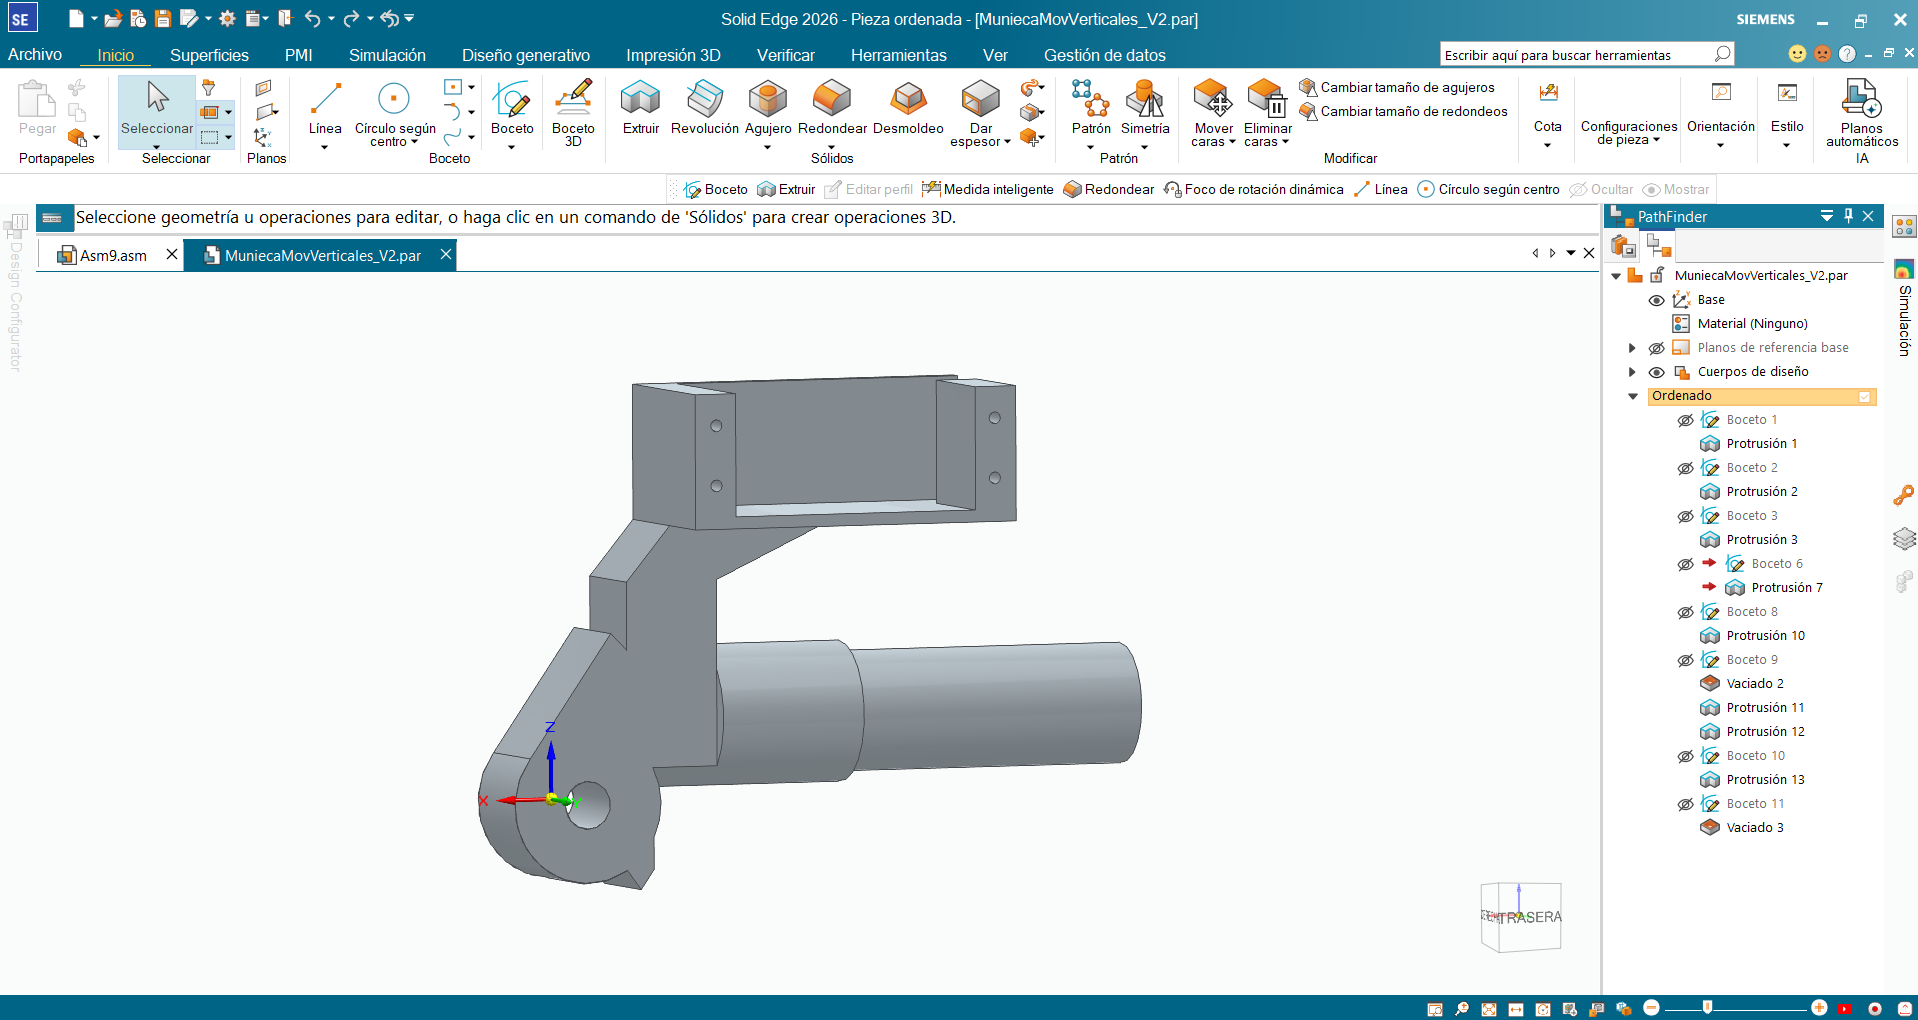
\includegraphics[scale=0.3]{SolidEdge.png}
 		\captionof{figure}{Entorno de Solid Edge.}
        \label{fig:SolidEdge}
    \end{center}
\end{figure}

En Solid Edge se dibujan bocetos en un plano y luego, mediante extrusiones, se los lleva de dos a tres dimensiones. Sobre una misma pieza se trazan bocetos en distintas caras y, con extrusiones, se realizan vaciados o protrusiones hasta obtener la forma deseada. De esta manera se desarrolló la estructura de la figura~\ref{fig:mano}.

\begin{figure}[H]
 \centering
  \subfigure[Vista lateral]{
    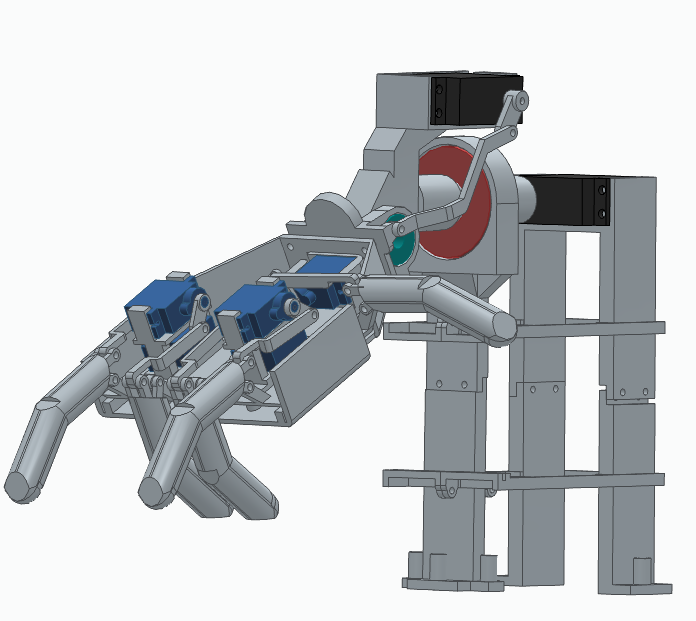
\includegraphics[width=0.42\textwidth]{Receptor/Receptor_1.png}}
  \subfigure[Vista posterior]{
    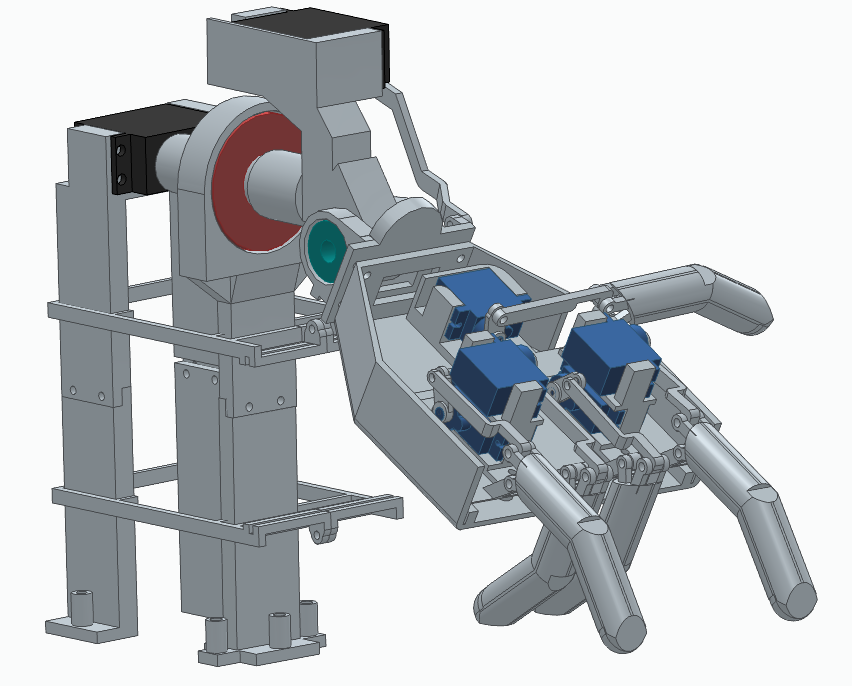
\includegraphics[width=0.48\textwidth]{Receptor/Receptor_2.png}}
 \caption{Diseño de la mano robótica y su soporte.}
 \label{fig:mano}
\end{figure}

La estructura se apoya sobre dos soportes de unos \SI{17}{\centi\meter} de altura. Para la rotación, un servo MG946R mueve un brazo de forma directa; para facilitar el giro se utiliza un rodamiento de \SI{20}{\milli\meter} de diámetro interior, y el brazo se une con la mano mediante un tornillo que pasa a través de ambos. El brazo contiene además el segundo servo MG946R, que mediante una biela produce el desplazamiento vertical de la mano.

Dentro de la palma, una base reúne los servos SG90 de los dedos. Los servos se ubican de a pares en forma vertical, uno en cada dirección, y cada uno se enlaza a su dedo mediante una biela; los dedos están atornillados a la base. El pulgar es la excepción: su servo se atornilla directamente a la base. También se diseñaron pequeños soportes que se enganchan a los soportes principales para sostener la base del microcontrolador. Todas las piezas se imprimieron en una impresora Hellbot Hidra.

\begin{figure}[H]
 \centering
  \subfigure[Muñeca]{
    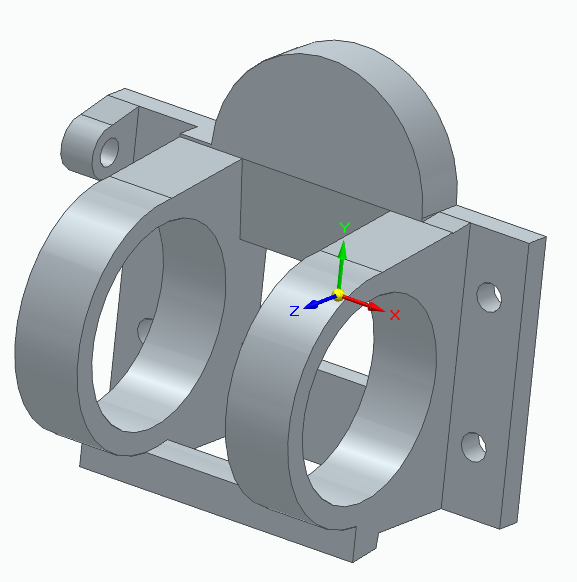
\includegraphics[width=0.22\textwidth]{Receptor/Muñeca.png}}
  \subfigure[Antebrazo]{
    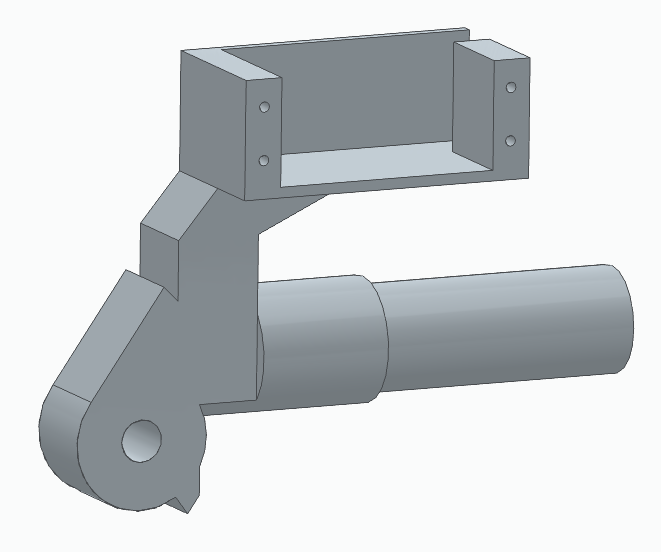
\includegraphics[width=0.22\textwidth]{Receptor/Antebrazo.png}}
  \subfigure[Palma]{
    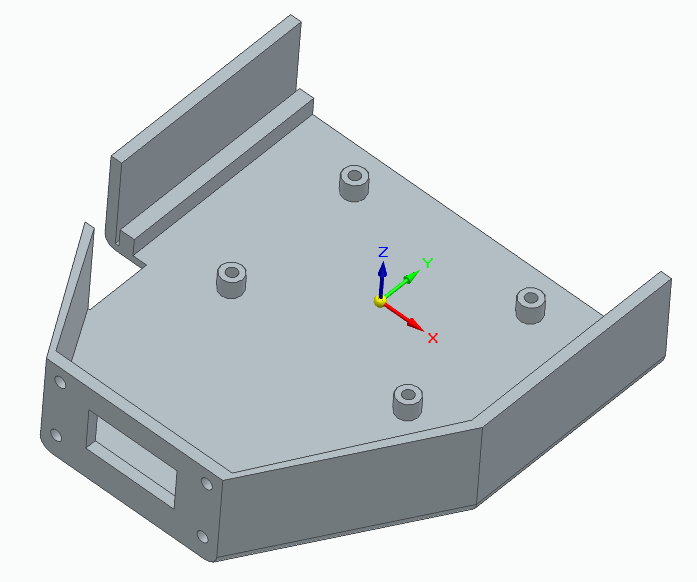
\includegraphics[width=0.22\textwidth]{Receptor/Palma.png}}
  \subfigure[Base de la mano]{
    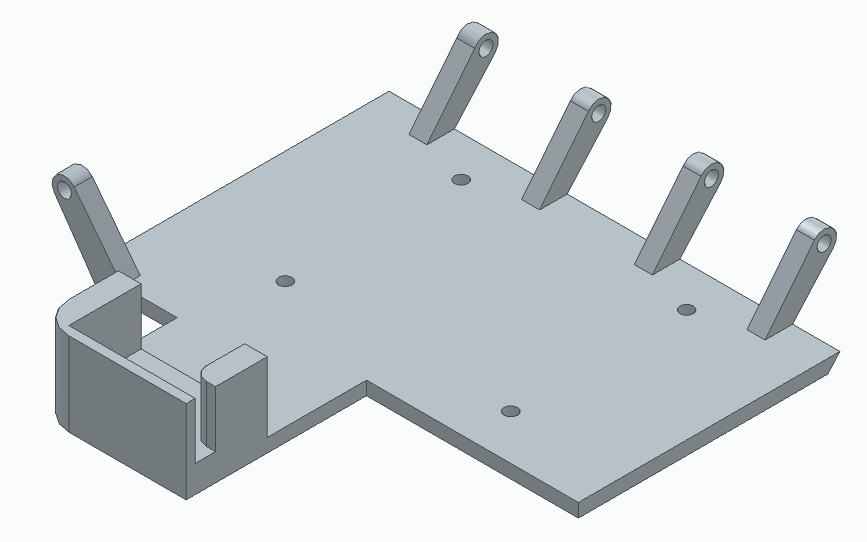
\includegraphics[width=0.22\textwidth]{Receptor/BaseMano.png}}
  \subfigure[Dedo]{
    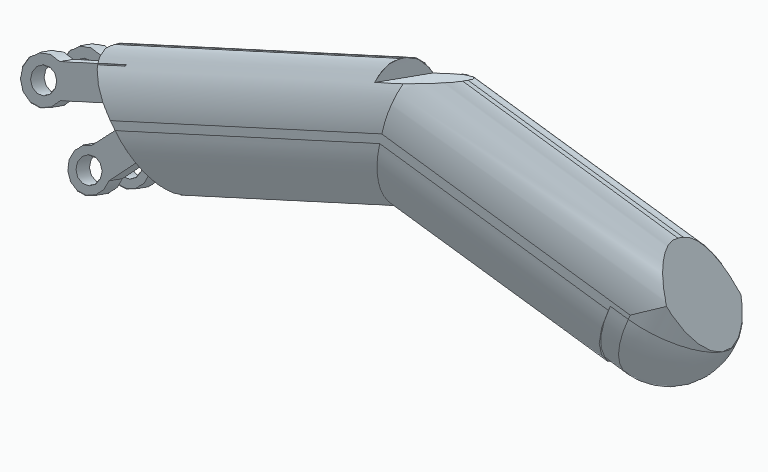
\includegraphics[width=0.22\textwidth]{Receptor/Dedo.png}}
  \subfigure[Base de servo]{
    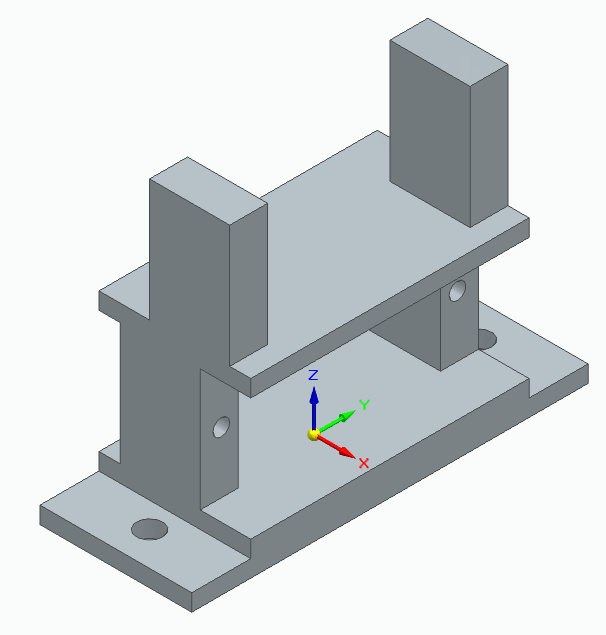
\includegraphics[width=0.22\textwidth]{Receptor/BaseServo.png}}
  \subfigure[Soporte]{
    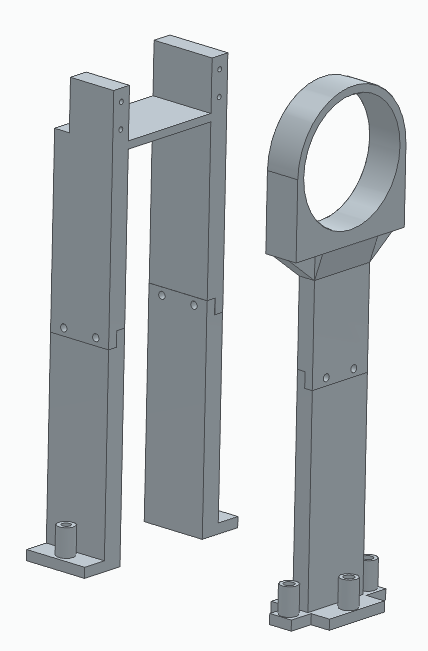
\includegraphics[width=0.22\textwidth]{Receptor/Soporte.png}}
 \caption{Piezas de la mano robótica.}
 \label{fig:piezas_mano}
\end{figure}

\pendiente{Revisar los nombres de las subfiguras y agregar una breve descripción de cada pieza si corresponde. Las imágenes \texttt{Diseño\_Receptor\_*.png} y \texttt{PrimerModeloMano\_*.png} quedaron sin usar: incluirlas si se quiere mostrar la evolución del diseño.}

\begin{figure}[H]
 \centering
  \subfigure[Base ESP32]{
    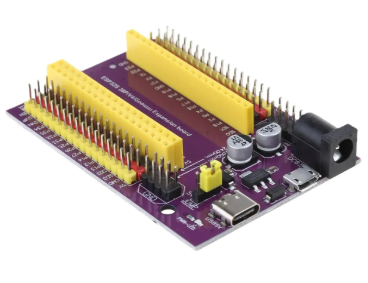
\includegraphics[width=0.3\textwidth]{ESP32_Base.png}}
  \subfigure[Impresora 3D Hellbot Hidra]{
    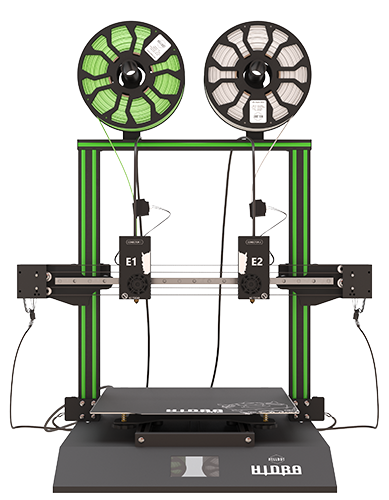
\includegraphics[width=0.2\textwidth]{Hidra_Hellbot.png}}
 \caption{Placa base del ESP32 e impresora utilizada.}
 \label{f:Extra}
\end{figure}

Como el software sólo limita los dedos al rango de \SIrange{25}{90}{\degree}, el diseño de las piezas debe permitir un recorrido libre algo mayor (por ejemplo, de \SIrange{20}{95}{\degree}), de manera que el servo nunca llegue a forzar la estructura de plástico y dañe sus engranajes.

\subsection{Conexionado y alimentación}
\label{sec:alimentacion}

El uso de la placa base del ESP32 (figura~\ref{f:Extra}) simplificó el conexionado, ya que ofrece tiras de pines con señal, alimentación y masa en la disposición que requieren los servos. La alimentación se dividió en dos:

\begin{itemize}
    \item \textbf{Servos:} una fuente externa de \SI{12}{\volt} y \SI{4}{\ampere} alimenta un regulador conmutado reductor (\textit{buck}) basado en el MP1584, cuya salida de \SI{5}{\volt} se conecta a los pines de alimentación de la placa base, de donde la toman los siete servos.
    \item \textbf{ESP32:} se alimenta por su conector micro-USB. Durante las pruebas lo alimenta la computadora, que también recibe la telemetría; en el diseño final se prevé un \textit{powerbank} o un paquete de baterías.
\end{itemize}

Las masas de ambas alimentaciones están unidas, ya que la señal PWM de cada servo se mide respecto del GND del ESP32. Para que las dos alimentaciones no queden conectadas entre sí, se removió el pin 5V de la placa del ESP32: de lo contrario, ese pin quedaría unido a los \SI{5}{\volt} de la placa base y el regulador podría inyectar corriente al puerto USB de la computadora.

\begin{figure}[H]
 \centering
  \subfigure[]{
    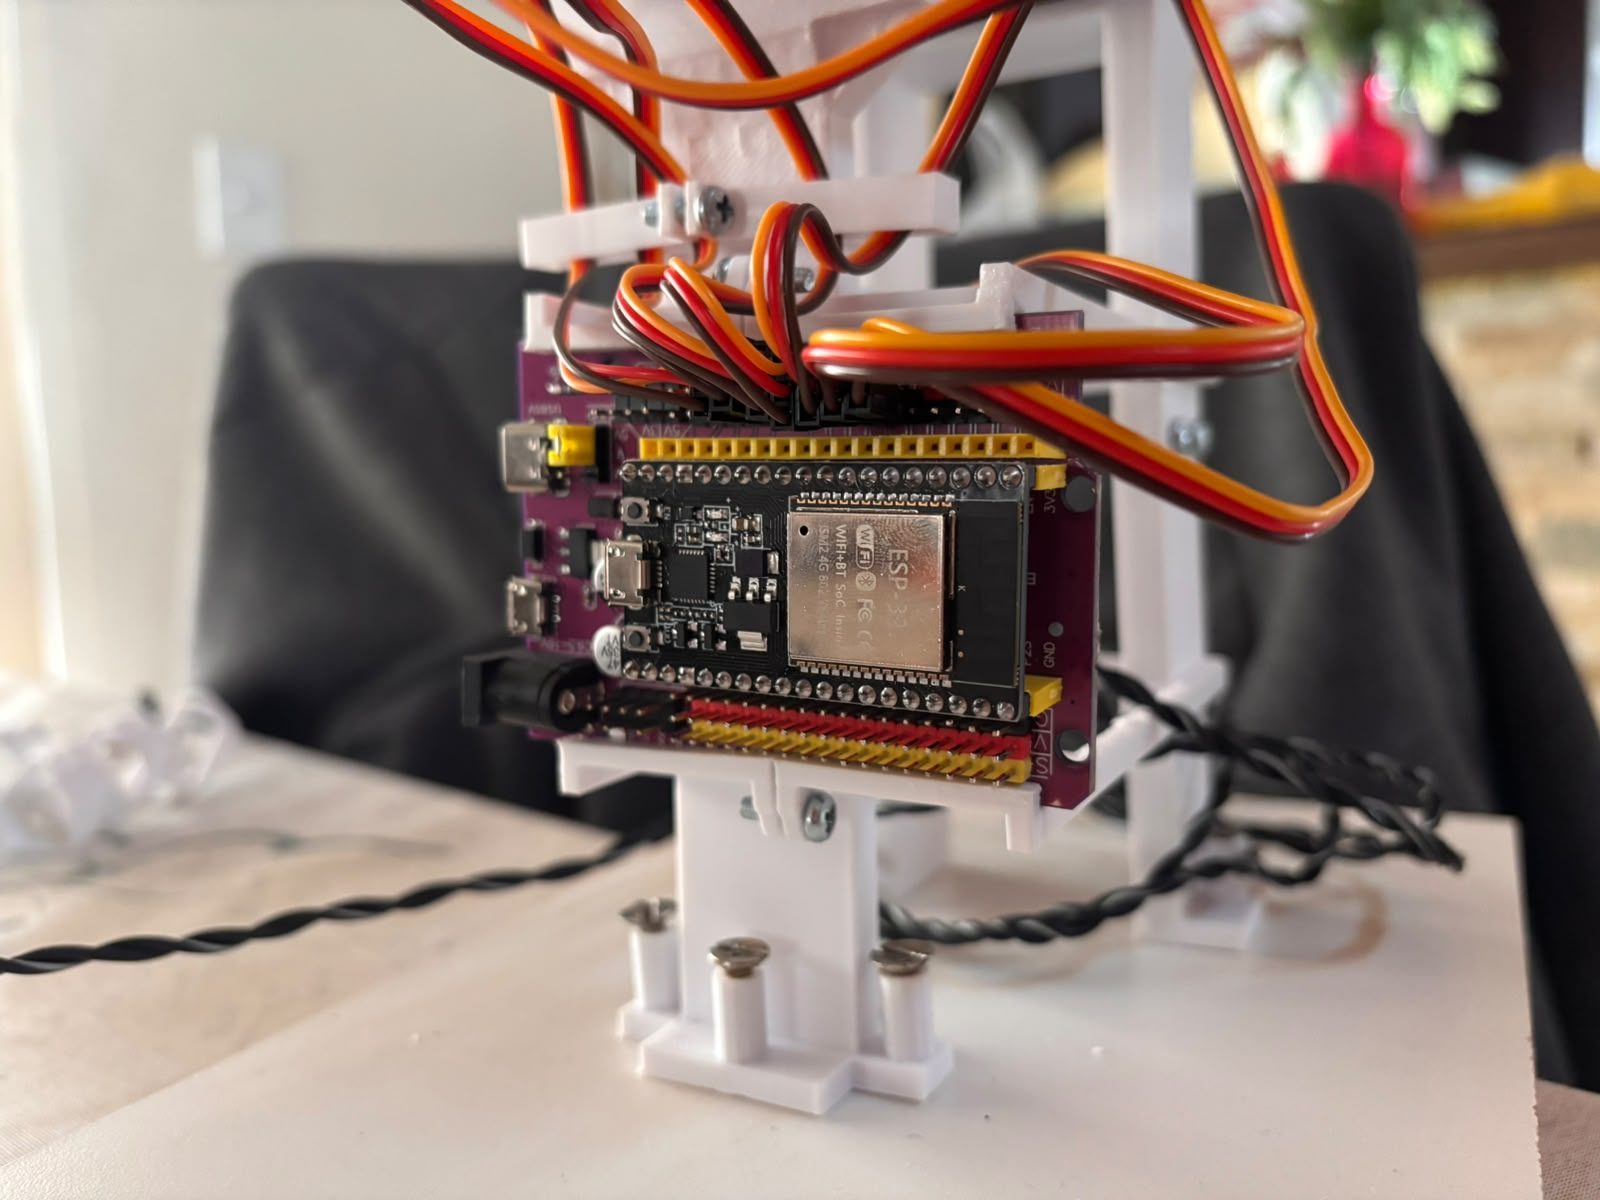
\includegraphics[width=0.45\textwidth]{Conexionado_Receptor_1.jpeg}}
  \subfigure[]{
    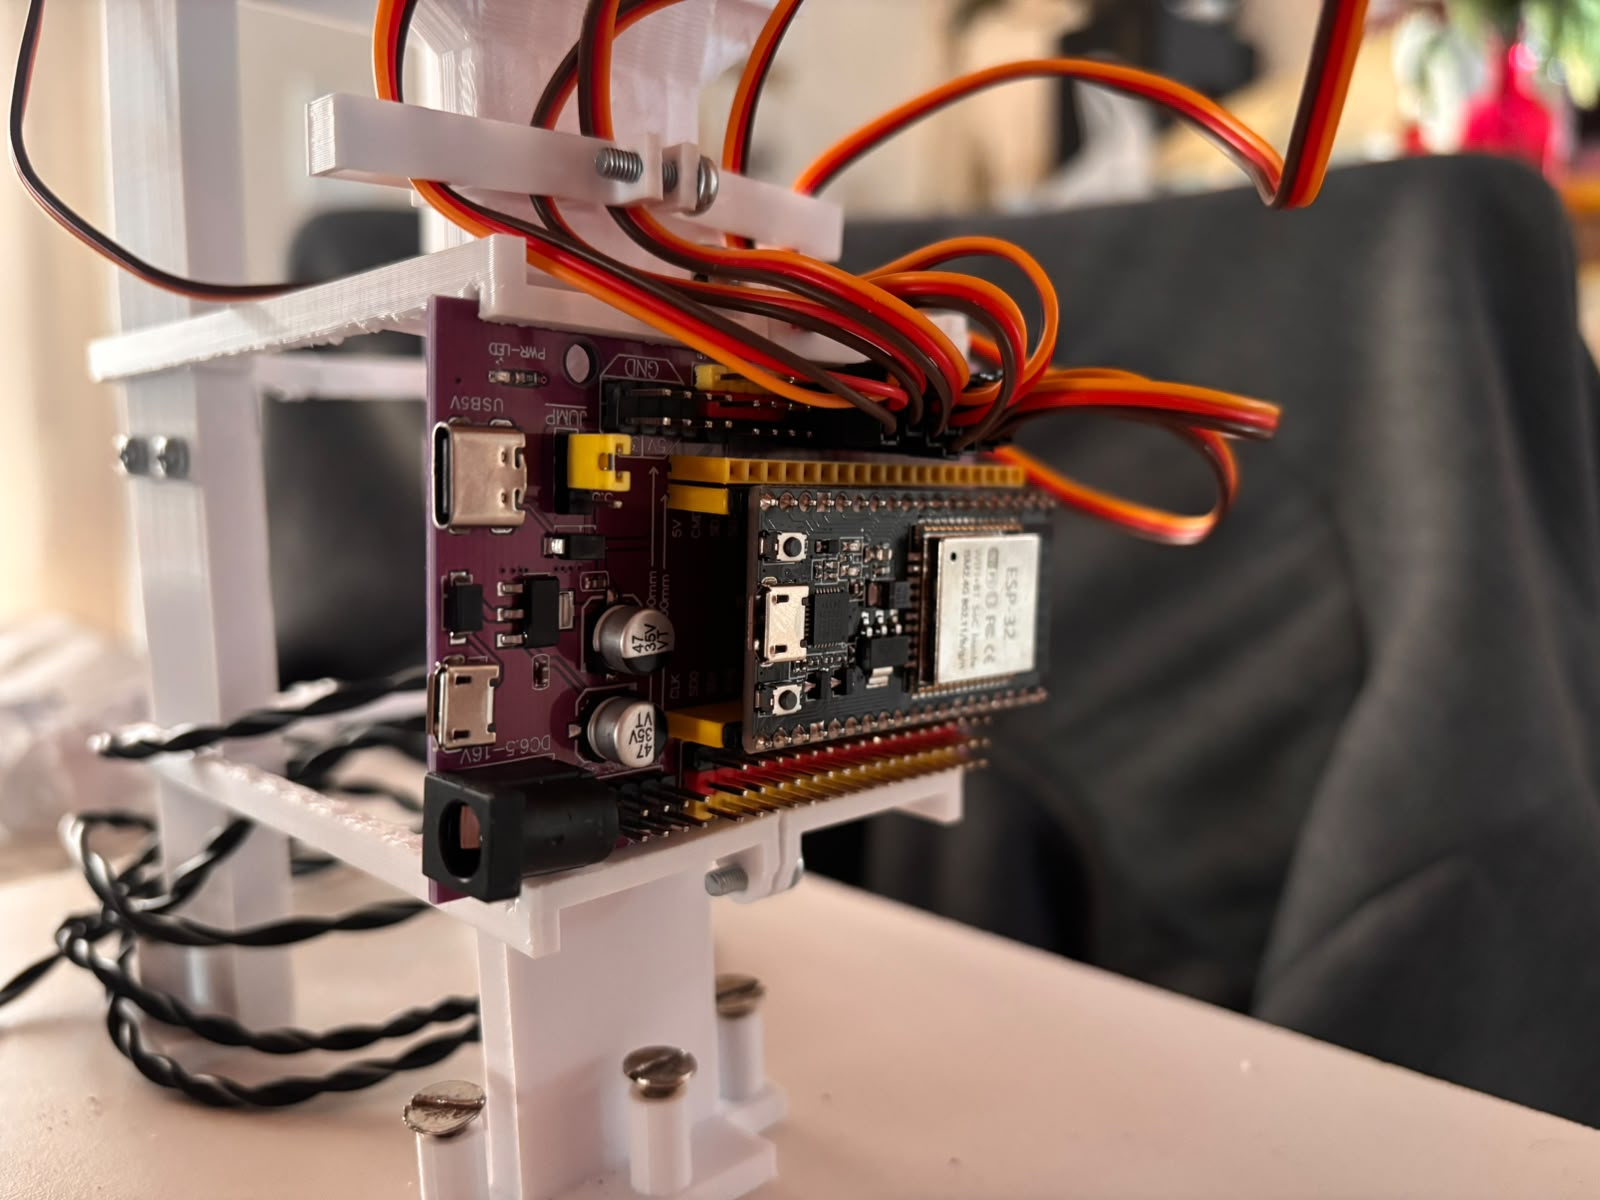
\includegraphics[width=0.45\textwidth]{Conexionado_Receptor_2.jpeg}}
 \caption{Conexionado del receptor.}
 \label{fig:conexionado_rx}
\end{figure}

La figura~\ref{fig:diagrama_rx} muestra el diagrama de conexionado del receptor, con las dos alimentaciones separadas.

\begin{figure}[H]
    \centering
    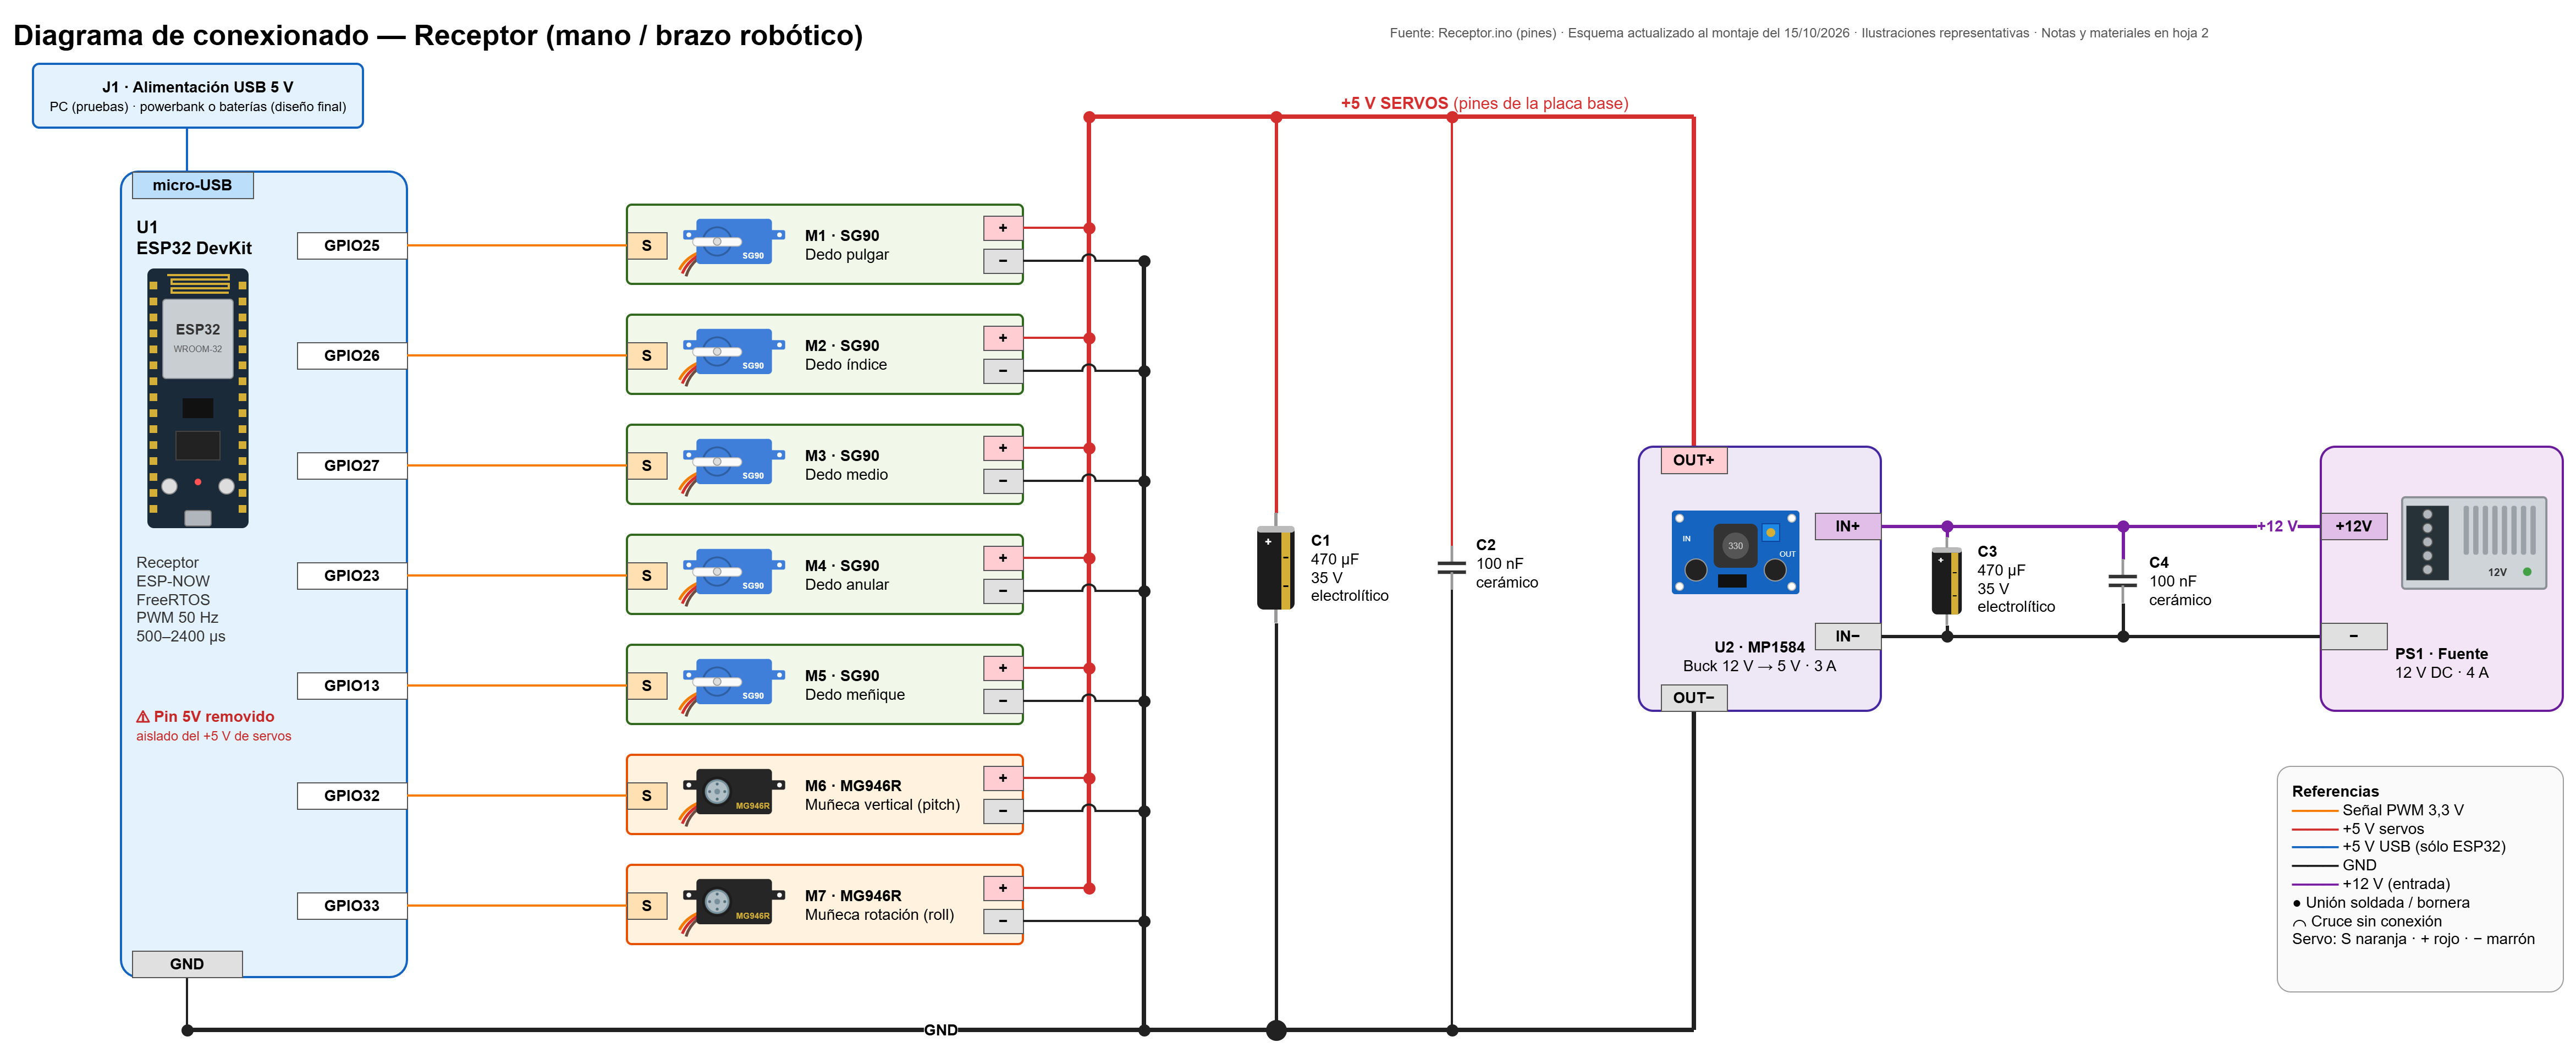
\includegraphics[width=\textwidth]{Conexionado_Receptor_Diagrama.png}
    \caption{Diagrama de conexionado del receptor.}
    \label{fig:diagrama_rx}
\end{figure}

La tabla~\ref{tab:pines_rx} indica el pin asignado a cada servo. Se eligieron los pines más cercanos a cada cable, ya que estos miden unos \SI{30}{\centi\meter} y no deben desconectarse cuando la mano se mueve.

\begin{table}[H]
\centering
\begin{tabular}{l c}
\toprule
\textbf{Servo} & \textbf{GPIO} \\
\midrule
Pulgar, índice, medio & 25, 26, 27 \\
Anular, meñique & 12, 13 \\
Muñeca vertical & 32 \\
Muñeca rotacional & 33 \\
\bottomrule
\end{tabular}
\caption{Asignación de pines del receptor.}
\label{tab:pines_rx}
\end{table}

El GPIO 12 es un pin de configuración de arranque (\textit{strapping}) del ESP32, que define la tensión de la memoria flash al iniciar \cite{esp32_datasheet}. Si se mantuviera en nivel alto durante el reinicio, la placa podría no arrancar. En las pruebas no causó inconvenientes, pero debe tenerse en cuenta ante una falla de arranque.

\begin{figure}[H]
    \begin{center}
 		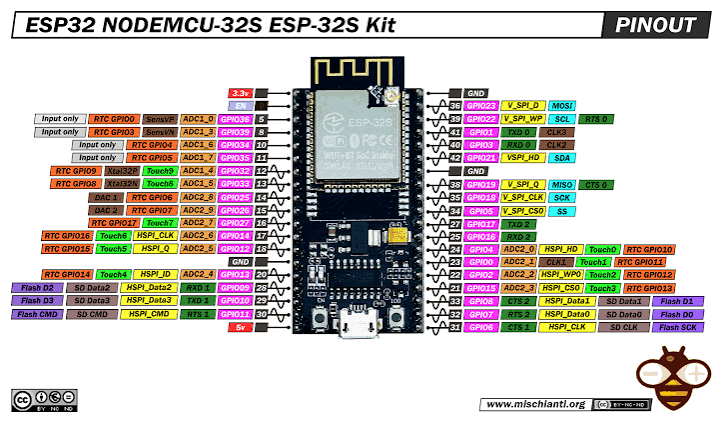
\includegraphics[scale=0.5]{ESP32_Pinout.png}
 		\captionof{figure}{Distribución de pines del ESP32.}
        \label{fig:pinout}
    \end{center}
\end{figure}

\subsubsection{Consumo}

La tabla~\ref{tab:consumos} resume los valores eléctricos de los componentes del receptor según sus fabricantes.

\begin{table}[H]
\centering
\begin{tabularx}{\textwidth}{l X X}
\toprule
\textbf{Componente} & \textbf{Valores} & \textbf{Fuente} \\
\midrule
SG90 (dedos) & \SI{4.8}{\volt}; \SI{1.8}{\kilo\gram\centi\meter} de torque de bloqueo. El fabricante no publica corrientes. Un distribuidor informa \SIrange{100}{250}{\milli\ampere} en movimiento y \SI{360}{\milli\ampere} bloqueado (medido por el distribuidor). & \cite{sg90_datasheet}, \cite{sg90_protosupplies} \\
MG946R (muñeca) & \SIrange{4.8}{6.6}{\volt}; \SI{10}{\milli\ampere} en reposo, \SI{170}{\milli\ampere} en operación sin carga y \SI{1.2}{\ampere} bloqueado; \SI{10.5}{\kilo\gram\centi\meter} a \SI{4.8}{\volt}. & \cite{mg946r_datasheet} \\
ESP32 & Alimentación del chip de \SIrange{2.3}{3.6}{\volt} (típica \SI{3.3}{\volt}); la fuente debe poder entregar al menos \SI{500}{\milli\ampere}. Consumo típico de la radio: \SI{240}{\milli\ampere} transmitiendo (802.11b, \SI{19.5}{dBm}) y \SIrange{95}{100}{\milli\ampere} recibiendo. & \cite{esp32_datasheet} (sec.~2.5.3, tablas 5-2 y 5-4) \\
MP1584 (regulador \textit{buck}) & Entrada de \SIrange{4.5}{28}{\volt}; \SI{3}{\ampere} de salida; frecuencia de conmutación programable de \SI{100}{\kilo\hertz} a \SI{1.5}{\mega\hertz}; límite de corriente del interruptor de \SI{4.0}{\ampere} mínimo (\SI{4.7}{\ampere} típico); apagado térmico a \SI{150}{\celsius}. & \cite{mp1584_datasheet} \\
\bottomrule
\end{tabularx}
\caption{Valores eléctricos de los componentes del receptor.}
\label{tab:consumos}
\end{table}

Para el SG90, la corriente de bloqueo varía entre fuentes no oficiales (de \SI{360}{\milli\ampere} a \SI{750}{\milli\ampere}), por lo que el valor medido en el propio montaje es más confiable que el de cualquier hoja de datos. Por otro lado, el valor mínimo de \SI{500}{\milli\ampere} del ESP32 cubre los picos de la radio (hasta \SI{379}{\milli\ampere} en transmisión continua según la hoja del módulo \cite{esp32_wroom_datasheet}).

Dado que los SG90 de los dedos no llegan al bloqueo, se los considera con consumo normal. En cambio, debe tenerse en cuenta la corriente de bloqueo de los MG946R, sobre todo la del servo de desplazamiento vertical, que es el que carga más peso. Considerando todo lo anterior, la fuente de los servos debe poder entregar al menos unos \SI{3}{\ampere}, que es la corriente nominal del MP1584. Con la corriente de bloqueo de los dos MG946R (\SI{2.4}{\ampere}) más el consumo de los cinco SG90 en movimiento, un pico simultáneo puede acercarse a ese valor o superarlo; por eso es importante limitar los picos.

Además del consumo medio, deben considerarse los picos de arranque: cuando varios servos arrancan a la vez, la corriente puede superar por algunos milisegundos la capacidad de la fuente. Si el ESP32 tomara su alimentación de esa misma línea de \SI{5}{\volt} y la tensión cayera lo suficiente, su regulador de \SI{3.3}{\volt} perdería regulación y el circuito de protección del microcontrolador provocaría un reinicio por baja tensión (\textit{brownout}); alimentarlo por USB separa su alimentación de la de los servos. Para limitar los picos se combinan dos medidas:

\begin{itemize}
    \item \textbf{En firmware}, el limitador de velocidad del receptor (sección~\ref{sec:slew}) impide que los servos reciban escalones grandes de posición, lo que reduce la aceleración pedida a los motores y, por lo tanto, los picos de corriente.
    \item \textbf{En hardware}, dos pares de capacitores iguales, cada uno formado por un electrolítico de \SI{470}{\micro\farad} / \SI{35}{\volt} en paralelo con un cerámico de \SI{100}{\nano\farad}:
    \begin{itemize}
        \item \textbf{A la salida del regulador}, sobre la línea de \SI{5}{\volt} de los servos y junto a los pines de la placa base. El electrolítico entrega la corriente de los picos de corta duración, que el regulador no alcanza a seguir, y el cerámico filtra el ruido de alta frecuencia que generan los motores y la conmutación del regulador.
        \item \textbf{A la entrada del regulador}, entre IN+ e IN$-$. Entrega los pulsos de corriente de la conmutación del regulador, de modo que la fuente de \SI{12}{\volt} y sus cables vean una corriente más pareja.
    \end{itemize}
\end{itemize}

El consumo medido sobre el montaje se presenta en la sección~\ref{sec:pruebas_alimentacion}. En resumen, a \SI{12}{\volt} el receptor consume en promedio unos \SIrange{75}{100}{\milli\ampere} en reposo y unos \SI{0.2}{\ampere} moviendo la muñeca en sus dos ejes, con picos de \SIrange{0.6}{0.7}{\ampere}. Estos valores están muy por debajo de los \SI{4}{\ampere} de la fuente y de los \SI{3}{\ampere} del regulador.

\subsection{Firmware del receptor}

\subsubsection{Arquitectura: callback, cola y tarea de control}

La figura~\ref{fig:arquitectura_rx} muestra el recorrido de un paquete dentro del receptor.

\begin{figure}[H]
\centering
\begin{tikzpicture}[node distance=0.6cm and 1.5cm, every node/.style={font=\small}]
  \node[bloque] (radio) {Radio\\ESP-NOW};
  \node[bloque, right=0.8cm of radio, fill=orange!10] (cb) {Callback\\\texttt{OnDataRecv}\\(tarea Wi-Fi, núcleo 0)\\Valida tamaño,\\firma y checksum};
  \node[bloque, right=of cb, fill=yellow!15] (cola) {Cola\\(1 elemento)};
  \node[bloque, right=of cola, fill=green!10] (ctrl) {Tarea de control\\(núcleo 1)\\Failsafe, trayectoria\\y escritura PWM};
  \node[bloque, below=of ctrl] (servos) {7 servos};
  \draw[flecha] (radio) -- (cb);
  \draw[flecha] (cb) -- node[below, font=\footnotesize]{sobrescribe} (cola);
  \draw[flecha] (cola) -- node[below, font=\footnotesize]{despierta} (ctrl);
  \draw[flecha] (ctrl) -- (servos);
\end{tikzpicture}
\caption{Recorrido de un paquete en el receptor.}
\label{fig:arquitectura_rx}
\end{figure}

\paragraph{Recepción.} El callback de recepción de ESP-NOW se ejecuta dentro de la tarea de Wi-Fi \cite{espnow_idf}, por lo que debe ser breve: descarta los paquetes cuyo tamaño no es de 19 bytes o cuya firma o suma de verificación no son válidas, y copia el paquete válido en una cola de FreeRTOS.

\paragraph{Cola de un elemento.} Si el callback escribiera directamente las variables que usa la tarea de control, ésta podría leer un paquete a medio escribir (condición de carrera). La cola copia el paquete completo de forma atómica. Su longitud es uno y se escribe con \texttt{xQueueOverwrite}, de modo que funciona como un buzón que guarda sólo el último paquete \cite{freertos}: si llegan dos antes de que la tarea los lea, el más viejo se descarta en lugar de acumularse, lo que generaría un retardo creciente.

\paragraph{Tarea de control.} La tarea queda bloqueada esperando la cola durante, como máximo, \SI{20}{\milli\second}. Si llega un paquete, despierta en ese mismo instante y lo procesa; si no llega ninguno, el tiempo de espera vence y la tarea itera igual, de modo que la supervisión del enlace y el movimiento hacia la posición de reposo siguen funcionando a \SI{50}{\hertz}.

\begin{lstlisting}[caption={Espera de paquetes en la tarea de control.}, label={cod:cola}]
if (xQueueReceive(colaMensajesBrazo, &paqueteEntrante,
                  pdMS_TO_TICKS(PERIODO_CONTROL_MS)) == pdTRUE) {
    marcaTiempoUltimoPaquete = millis();
    // ... pasar a operación normal si hacía falta y actualizar objetivos
    posObjetivoMuniecaVert = constrain((float)paqueteEntrante.muniecaVertical,
                                       LIM_MUNIECA_VERT_MIN, LIM_MUNIECA_VERT_MAX);
}
\end{lstlisting}

Al recibir un paquete, las posiciones objetivo se saturan a los límites mecánicos de la mano (\SIrange{25}{90}{\degree} para los dedos y la muñeca vertical, \SIrange{0}{180}{\degree} para la rotación), como protección adicional ante un valor fuera de rango.

\subsubsection{Máquina de estados y modo de seguridad}
\label{sec:fsm}

La tarea de control supervisa el enlace con la máquina de estados de la figura~\ref{fig:fsm}.

\begin{figure}[H]
\centering
\begin{tikzpicture}[node distance=1.6cm and 2.2cm, every node/.style={font=\small},
  estado/.style={draw, rounded corners=8pt, align=center, minimum width=3cm, minimum height=1.1cm, fill=blue!5}]
  \node[estado] (sync) {\texttt{ESPERANDO\_SYNC}\\Servos en reposo};
  \node[estado, right=of sync, fill=green!10] (normal) {\texttt{OPERACION\_NORMAL}\\Sigue al guante};
  \node[estado, below=of normal, fill=red!10] (fs) {\texttt{FAILSAFE\_SIN\_SENAL}\\Objetivos en reposo};
  \node[estado, right=of fs, fill=gray!15, dashed] (desac) {Servos desacoplados\\(sin PWM)};
  \draw[flecha] ($(sync.north)+(0,0.7)$) -- node[right, font=\footnotesize]{Inicio} (sync);
  \draw[flecha] (sync) -- node[above, font=\footnotesize]{Paquete válido} (normal);
  \draw[flecha] ($(normal.south)+(0.5,0)$) -- node[right, font=\footnotesize, align=left]{$>\SI{250}{\milli\second}$\\sin paquetes} ($(fs.north)+(0.5,0)$);
  \draw[flecha] ($(fs.north)+(-0.5,0)$) -- node[left, font=\footnotesize]{Paquete válido} ($(normal.south)+(-0.5,0)$);
  \draw[flecha] (fs) -- node[above, font=\footnotesize, align=center]{En reposo y\\$>\SI{2}{\second}$} (desac);
  \draw[flecha] (desac.north) |- node[pos=0.25, right, font=\footnotesize, align=left]{Paquete válido\\(reacopla)} (normal.east);
\end{tikzpicture}
\caption{Máquina de estados del receptor. El estado ``desacoplado'' no es un estado del código: es el modo de seguridad con los servos apagados.}
\label{fig:fsm}
\end{figure}

\begin{itemize}
    \item Al encender, los servos se energizan en la posición de reposo (dedos en \SI{25}{\degree}, muñeca vertical en \SI{57}{\degree} y rotación en \SI{90}{\degree}) y se espera el primer paquete válido.
    \item Si en operación normal pasan más de \SI{250}{\milli\second} sin paquetes válidos (unos 12 paquetes perdidos seguidos), se considera perdido el enlace: por ejemplo, porque el guante se apagó o salió de alcance. Las posiciones objetivo pasan a la de reposo y la mano se mueve hacia ella de forma suave. Este tiempo tolera interferencias breves y reacciona rápido ante un corte real.
    \item Si el modo de seguridad se mantiene, todos los servos llegaron a la posición de reposo y pasaron más de \SI{2}{\second} desde que se entró en él, se interrumpe la señal PWM (\texttt{detach}). Sin señal, los servos dejan de sostener la posición, de consumir corriente y de calentarse.
    \item En cualquier caso, al llegar un paquete válido se vuelve a operación normal y, si hacía falta, se vuelven a acoplar los servos, que arrancan desde la última posición escrita para no dar un salto.
\end{itemize}

\subsubsection{Generador de trayectoria: limitador de velocidad y banda muerta}
\label{sec:slew}

En cada iteración, para cada servo $i$, se calcula el error entre la posición objetivo y la actual y se avanza a lo sumo $\Delta\theta_{\max}$ grados:
\begin{equation}
e_i[k] = \theta^{obj}_i - \theta_i[k-1], \qquad
\theta_i[k] =
\begin{cases}
\theta_i[k-1] + \operatorname{sat}_{[-\Delta\theta_{\max},\,\Delta\theta_{\max}]}\left(e_i[k]\right) & \text{si } |e_i[k]| > \delta \\
\theta_i[k-1] & \text{si } |e_i[k]| \leq \delta
\end{cases}
\end{equation}

\paragraph{Limitador de velocidad (\textit{slew-rate limiter}).} Ante un salto grande del objetivo, por ejemplo al reconectarse o al entrar en el modo de seguridad, el movimiento resultante es una rampa y no un escalón. Esto limita los picos de corriente y el esfuerzo sobre los engranajes y las piezas impresas. Los límites elegidos (tabla~\ref{tab:param_rx}) son cercanos a la velocidad propia de los servos, de modo que en uso normal casi no agregan retardo.

\paragraph{Banda muerta (\textit{deadband}).} Si el error es menor o igual a $\delta$ no se escribe una nueva posición. Sin esta banda, el ruido residual del guante haría que el servo corrija décimas de grado constantemente y zumbe (\textit{hunting}), calentándose. Como contrapartida, la posición final puede diferir del objetivo hasta en $\delta$.

\begin{table}[H]
\centering
\begin{tabular}{l c c c}
\toprule
\textbf{Servo} & $\boldsymbol{\Delta\theta_{\max}}$ \textbf{por ciclo} & \textbf{Velocidad máxima} & \textbf{Banda muerta} $\boldsymbol{\delta}$ \\
\midrule
Dedos (SG90)              & \SI{8}{\degree} & \SI{400}{\degree\per\second} & \SI{1.0}{\degree} \\
Muñeca vertical (MG946R)  & \SI{4}{\degree} & \SI{200}{\degree\per\second} & \SI{1.2}{\degree} \\
Muñeca rotacional (MG946R)& \SI{5}{\degree} & \SI{250}{\degree\per\second} & \SI{1.2}{\degree} \\
\bottomrule
\end{tabular}
\caption{Parámetros del generador de trayectoria (ciclo de \SI{20}{\milli\second}).}
\label{tab:param_rx}
\end{table}

\subsubsection{Inversión del sentido de los dedos}

Todo el sistema trabaja con la convención lógica de \SI{25}{\degree} = dedo abierto y \SI{90}{\degree} = dedo cerrado. Según cómo esté montado cada servo en la palma, puede ocurrir que cierre el dedo al \emph{disminuir} su ángulo. Para no modificar la mecánica, el arreglo \texttt{INVERTIR\_DEDO} indica, para cada dedo, si el ángulo debe espejarse dentro del rango justo antes de escribirlo en el servo:
\begin{equation}
\theta_{servo} =
\begin{cases}
25 + 90 - \theta & \text{si el dedo está invertido} \\
\theta & \text{en otro caso.}
\end{cases}
\end{equation}
Como la inversión se aplica sólo en la escritura, la posición de reposo, los límites, el modo de seguridad y la telemetría siguen expresados en la convención lógica.

\subsubsection{Generación de PWM}

Los servos se controlan con la librería \texttt{ESP32Servo}, que genera la señal con el periférico LEDC del ESP32. Al inicio se reservan cuatro temporizadores de hardware para este fin. Cada servo se configura a \SI{50}{\hertz} con pulsos de \SI{500}{\micro\second} para \SI{0}{\degree} y \SI{2400}{\micro\second} para \SI{180}{\degree}, es decir, unos \SI{10.6}{\micro\second} por grado.

\section{Evolución del diseño}
\label{sec:evolucion}

El firmware se desarrolló de forma iterativa: cada versión se probó en el hardware y los problemas observados motivaron la siguiente. Las versiones están identificadas con etiquetas (\textit{tags}) en el repositorio de git del proyecto, lo que permite reproducir cualquiera de ellas. La tabla~\ref{tab:versiones} resume la evolución y las secciones siguientes explican cada cambio.

\begin{table}[H]
\centering
\begin{tabularx}{\textwidth}{l X X}
\toprule
\textbf{Versión} & \textbf{Cambios principales} & \textbf{Motivo} \\
\midrule
Preliminar & Filtro EMA en el guante y en la mano, bucle con \texttt{delay(20)}, envío de lecturas crudas del ADC & Primera implementación funcional \\
1.0.0 & Tareas FreeRTOS, cola, protocolo con checksum, limitador de velocidad y banda muerta, calibración en NVS, filtro de Kalman en la muñeca & Retardo y zumbido de la versión preliminar \\
2.0.0 & Filtro complementario, calibración del giróscopo, mapeo en punto flotante & La muñeca derivaba ``como un mouse'' \\
2.1.0 & Limitador de velocidad más rápido, inversión de dedos por software & La mano respondía lento; dedos invertidos \\
2.2.0 & El receptor procesa cada paquete al llegar; DLPF a \SI{44}{\hertz} & Reducir la latencia \\
2.3.0 & Transmisión pausada durante la calibración & Consola y mano confusas al calibrar \\
\bottomrule
\end{tabularx}
\caption{Versiones del firmware. La versión 2.2.0 fue la última validada en hardware; la 2.3.0 sólo agrega la pausa durante la calibración.}
\label{tab:versiones}
\end{table}

\subsection{Versión preliminar}

En la primera implementación, el transmisor leía los potenciómetros, les aplicaba un filtro de media móvil exponencial (EMA),
\begin{equation}
y[k] = \alpha\, x[k] + (1-\alpha)\, y[k-1],
\end{equation}
con $\alpha = 0{,}15$, y enviaba las lecturas del ADC sin convertir. El receptor convertía esas lecturas a ángulos y aplicaba un segundo filtro EMA ($\alpha = 0{,}2$ para los dedos y $0{,}3$ para la muñeca) antes de escribir los servos. Ambos programas usaban un bucle con \texttt{delay(20)} y, en el receptor, el callback de recepción copiaba el paquete directamente sobre una variable global. La tabla~\ref{tab:preliminar} resume los problemas encontrados.

\begin{table}[H]
\centering
\begin{tabularx}{\textwidth}{X X X}
\toprule
\textbf{Planteo inicial} & \textbf{Problema} & \textbf{Solución adoptada} \\
\midrule
Dos filtros EMA en cascada (guante y mano) & Los retardos de ambos filtros se suman. Además, el EMA se acerca al objetivo con pasos cada vez más pequeños, que caen dentro de la zona de insensibilidad del servo y lo hacen zumbar & Limitador de velocidad y banda muerta en el receptor (sección~\ref{sec:slew}) \\
Bucle con \texttt{delay(20)} & El período real es \SI{20}{\milli\second} más el tiempo de cómputo, y varía & Tareas FreeRTOS con \texttt{vTaskDelayUntil} \\
Callback que escribe una variable global & La tarea principal puede leer un paquete a medio escribir & Cola FreeRTOS de un elemento \\
Paquete sin verificación & Un paquete corrupto o ajeno se interpretaría como una orden válida & Firma, número de secuencia y checksum (sección~\ref{sec:protocolo}) \\
Conversión fija de 0--4095 a \SIrange{25}{90}{\degree} & No contempla las diferencias entre dedos ni entre usuarios & Calibración de dos puntos en NVS \\
\bottomrule
\end{tabularx}
\caption{Problemas de la versión preliminar.}
\label{tab:preliminar}
\end{table}

\subsection{Versión 1.0.0: filtro de Kalman}

La versión 1.0.0 incorporó la arquitectura descripta en las secciones~\ref{sec:transmisor} y~\ref{sec:receptor}, pero estimaba la orientación de la muñeca con un filtro de Kalman de dos estados por eje \cite{kalman1960}, según la implementación difundida por K.~Lauszus \cite{lauszus_kalman}. El filtro de Kalman es un estimador recursivo que pondera la predicción del modelo y la medición según sus incertidumbres. Su estado es el ángulo $\theta$ y el sesgo del giróscopo $b$, y en cada ciclo ejecuta dos etapas:

\begin{itemize}
    \item \textbf{Predicción:} con la velocidad angular medida $\omega$, se proyecta el ángulo y se actualiza la matriz de covarianza del error $P$, que crece según el ruido de proceso:
    \begin{equation}
    \theta^- = \theta + \Delta t\,(\omega - b), \qquad
    P^- = F P F^{T} + Q\,\Delta t, \qquad
    F = \begin{pmatrix} 1 & -\Delta t \\ 0 & 1 \end{pmatrix}, \quad
    Q = \begin{pmatrix} Q_{angle} & 0 \\ 0 & Q_{bias} \end{pmatrix}.
    \end{equation}
    \item \textbf{Corrección:} se compara la predicción con el ángulo del acelerómetro $\theta_{acc}$ y se corrigen ambos estados con la ganancia de Kalman $K$:
    \begin{equation}
    S = P^-_{00} + R, \qquad
    K = \frac{1}{S}\begin{pmatrix} P^-_{00} \\ P^-_{10} \end{pmatrix}, \qquad
    \begin{pmatrix} \theta \\ b \end{pmatrix} = \begin{pmatrix} \theta^- \\ b \end{pmatrix} + K\left(\theta_{acc} - \theta^-\right), \qquad
    P = \left(I - K H\right) P^-,
    \end{equation}
    con $H = \begin{pmatrix} 1 & 0 \end{pmatrix}$. Si la medición es ruidosa ($R$ grande), $K$ es pequeña y el filtro confía más en la predicción.
\end{itemize}

Los parámetros utilizados fueron $Q_{angle} = 0{,}001$, $Q_{bias} = 0{,}003$ y $R = 0{,}03$.

\begin{lstlisting}[caption={Etapas del filtro de Kalman (\texttt{KalmanFilter.h}, versión 1.0.0).}, label={cod:kalman}]
float getAngle(float newAngle, float newRate, float dt) {
    // 1. Predicción
    rate = newRate - bias;
    angle += dt * rate;
    P[0][0] += dt * (dt * P[1][1] - P[0][1] - P[1][0] + Q_angle);
    P[0][1] -= dt * P[1][1];
    P[1][0] -= dt * P[1][1];
    P[1][1] += Q_bias * dt;

    // 2. Corrección
    float S = P[0][0] + R_measure;
    float K[2] = { P[0][0] / S, P[1][0] / S };
    float y = newAngle - angle;
    angle += K[0] * y;
    bias  += K[1] * y;

    float P00_temp = P[0][0], P01_temp = P[0][1];
    P[0][0] -= K[0] * P00_temp;
    P[0][1] -= K[0] * P01_temp;
    P[1][0] -= K[1] * P00_temp;
    P[1][1] -= K[1] * P01_temp;
    return angle;
}
\end{lstlisting}

En las pruebas, la muñeca de la mano robótica se comportaba ``como un mouse'': derivaba y no volvía a la misma posición cuando el operador volvía a la misma postura. Al revisar el código se encontraron las siguientes causas:

\begin{enumerate}
    \item \textbf{Signo del giróscopo de \textit{pitch} invertido} respecto del ángulo del acelerómetro. El giróscopo empujaba la estimación en un sentido y el acelerómetro en el contrario, por lo que el resultado dependía de la historia del movimiento.
    \item \textbf{Variable sin inicializar en el \textit{roll}:} en la zona de singularidad se usaba el ángulo medido antes de asignarle un valor, lo que producía saltos.
    \item \textbf{Arranque desde \SI{0}{\degree}}, sin ángulo inicial ni calibración del \textit{bias}, con un transitorio al encender.
    \item \textbf{Conversión a enteros antes del mapeo}, que truncaba el ángulo a grados enteros y no lo saturaba antes de convertirlo.
\end{enumerate}

\subsection{Versión 2.0.0: filtro complementario}

Se reemplazó el filtro de Kalman por el filtro complementario de la sección~\ref{sec:fusion}. Un filtro de Kalman bien sintonizado no es inferior; sin embargo, para estimar dos ángulos de inclinación a \SI{50}{\hertz}, el filtro complementario da un resultado equivalente en la práctica, tiene un único parámetro ($\alpha$) con interpretación directa, en lugar de tres covarianzas, y es más fácil de verificar. Además se corrigieron los signos del giróscopo, se agregaron la calibración del \textit{bias} y la inicialización desde el acelerómetro, se retiene el \textit{roll} en la singularidad, se pasó a un mapeo en punto flotante saturado y ajustable, y en el receptor se agregaron los límites mecánicos de las posiciones objetivo.

\subsection{Versión 2.1.0: respuesta más rápida y dedos invertibles}

Las pruebas mostraron que la mano tardaba en seguir al guante. La causa era el limitador de velocidad, configurado por debajo de la velocidad de los propios servos: \SI{150}{\degree\per\second} para los dedos y \SI{75}{\degree\per\second} y \SI{100}{\degree\per\second} para la muñeca (un giro completo de \SI{180}{\degree} de la muñeca tardaba \SI{1.8}{\second}). Se elevaron a los valores de la tabla~\ref{tab:param_rx}. También se observó que, al cerrar un dedo del guante, el de la mano se abría, debido al sentido de montaje de los servos; se agregó la inversión por software. Por último, se desactivó el ahorro de energía de la radio también en el receptor.

\subsection{Versión 2.2.0: menor latencia}

Se aplicaron dos cambios de bajo riesgo para reducir la latencia:

\begin{itemize}
    \item Antes, la tarea del receptor despertaba cada \SI{20}{\milli\second} fijos y recién entonces consultaba la cola, lo que agregaba en promedio \SI{10}{\milli\second} (y hasta \SI{20}{\milli\second}) de espera. Ahora la tarea se bloquea esperando la cola y despierta al llegar el paquete.
    \item El filtro interno del MPU6050 pasó de \SI{21}{\hertz} a \SI{44}{\hertz}, unos \SI{3.5}{\milli\second} menos de retardo (tabla~\ref{tab:dlpf}).
\end{itemize}

Esta versión funcionó correctamente en la prueba en hardware.

\subsection{Versión 2.3.0: calibración sin transmisión}

Al calibrar con la versión 2.2.0, la telemetría se mezclaba con las instrucciones en la consola y la mano robótica imitaba los gestos de calibración. Se agregó una bandera que, durante la calibración, detiene la lectura de los dedos, el envío y la telemetría (sección~\ref{sec:calibracion_dedos}).

\section{Análisis temporal}
\label{sec:latencia}

La tabla~\ref{tab:latencia} estima el retardo desde que el operador mueve la mano hasta que el servo recibe la nueva orden. \textbf{Son estimaciones a partir del código y de las hojas de datos, no mediciones} sobre el hardware.

\begin{table}[H]
\centering
\begin{tabularx}{\textwidth}{X c X}
\toprule
\textbf{Etapa} & \textbf{Retardo} & \textbf{Origen} \\
\midrule
Espera hasta el siguiente ciclo del transmisor & 0--\SI{20}{\milli\second} (media 10) & Muestreo a \SI{50}{\hertz} \\
Filtro interno del MPU6050 (sólo muñeca) & $\approx\SI{5}{\milli\second}$ & DLPF de \SI{44}{\hertz} \cite{mpu6050_regmap} \\
Lectura de dedos, cálculo y empaquetado & $\approx\SI{5}{\milli\second}$ & Sobremuestreo $16\times$ \\
Transmisión ESP-NOW & $\approx$ 1--\SI{6}{\milli\second} & Valores típicos reportados \cite{espnow_faq, espnow_issue115} \\
Tarea de control del receptor & $<\SI{1}{\milli\second}$ & Despierta al llegar el paquete \\
Siguiente pulso PWM del servo & 0--\SI{20}{\milli\second} (media 10) & PWM de \SI{50}{\hertz} \\
Limitador de velocidad del receptor & 0--$\approx$\SI{160}{\milli\second} & \SI{8}{\degree} por ciclo en los dedos (tabla~\ref{tab:param_rx}): 0 para cambios chicos, unos 8 ciclos para un recorrido completo \\
Movimiento mecánico & según amplitud & $\approx\SI{0.1}{\second}$ cada \SI{60}{\degree} (SG90 sin carga) \\
\bottomrule
\end{tabularx}
\caption{Estimación de la cadena de retardos (versión 2.2.0 y posteriores).}
\label{tab:latencia}
\end{table}

En promedio, la orden llega al servo unos \SI{30}{\milli\second} después del movimiento del operador. Ante cambios grandes se suma el limitador de velocidad, que reparte el movimiento en varios ciclos, y luego el tiempo que tarda el servo en recorrer el ángulo.

Para medir la latencia real se preparó un ensayo de punta a punta sobre el camino de los dedos (procedimiento en \texttt{docs/\allowbreak pruebas/\allowbreak PRUEBA\_LATENCIA.md}). El receptor reemplaza al potenciómetro del índice: aplica un escalón de tensión en la entrada del transmisor (GPIO 34) y mide, con su propio reloj, el tiempo hasta el fin del primer pulso PWM con el ancho nuevo en la salida del servo del índice. Como el inicio y el fin se toman en la misma placa, no hace falta sincronizar relojes. La medición incluye la espera al ciclo del transmisor, la lectura y el envío, la recepción, la tarea de control y la espera al pulso PWM; no incluye el movimiento mecánico ni el filtro interno del MPU6050.

\pendiente{Faltan los resultados de este ensayo: con ellos se confirmará o corregirá esta estimación.}

\section{Pruebas}
\label{sec:pruebas}

Las pruebas se dividen en dos grupos. El primero corresponde a la versión preliminar del firmware (filtros EMA y filtro de Kalman) y se conserva como antecedente, ya que motivó los cambios descriptos en la sección~\ref{sec:evolucion}. El segundo corresponde a las pruebas realizadas con la versión 2.3.0: la respuesta del sistema completo y la alimentación del receptor.

\subsection{Versión preliminar del firmware}
\label{sec:pruebas_preliminar}

Se analizó la utilidad de los filtros para cada medición realizada en el ESP32. Primero se observaron las mediciones del MPU6050 con el módulo totalmente quieto y luego con un pequeño movimiento. Para el \textit{pitch} resulta:

\begin{figure}[H]
 \centering
  \subfigure[\textit{Pitch} sin movimiento]{
    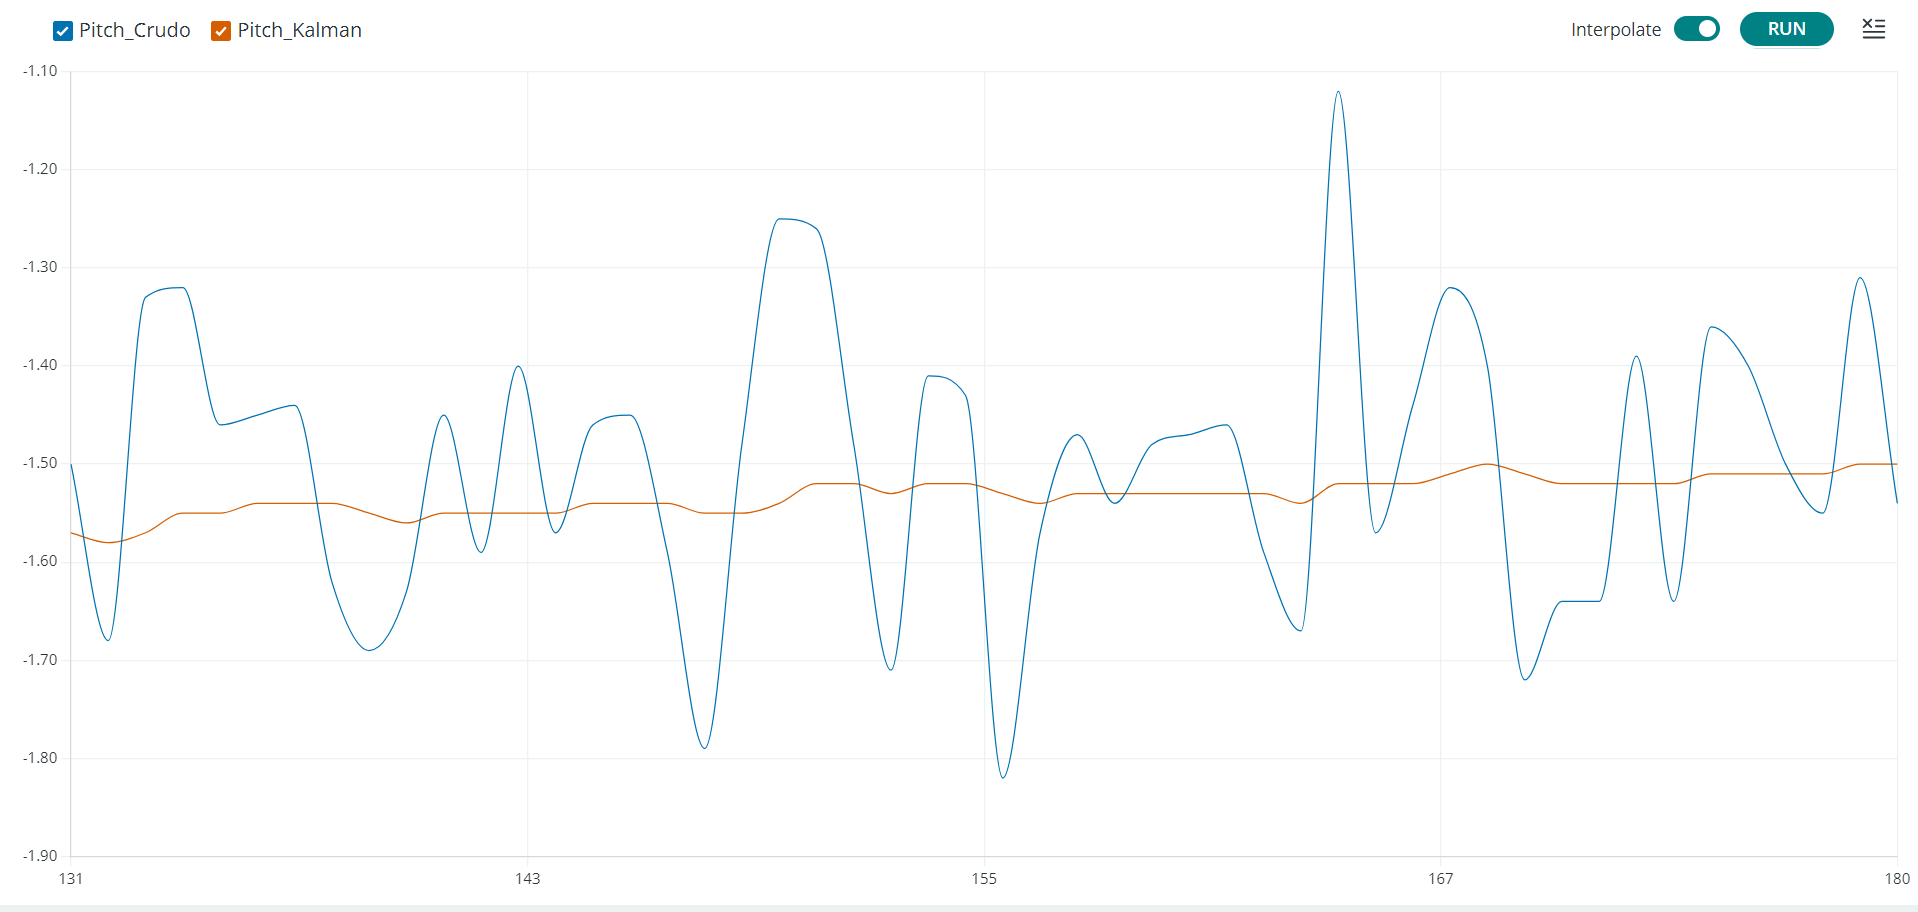
\includegraphics[width=0.45\textwidth]{Pitch_Ruido_Sin_Movimiento.png}}
  \subfigure[\textit{Pitch} con movimiento]{
    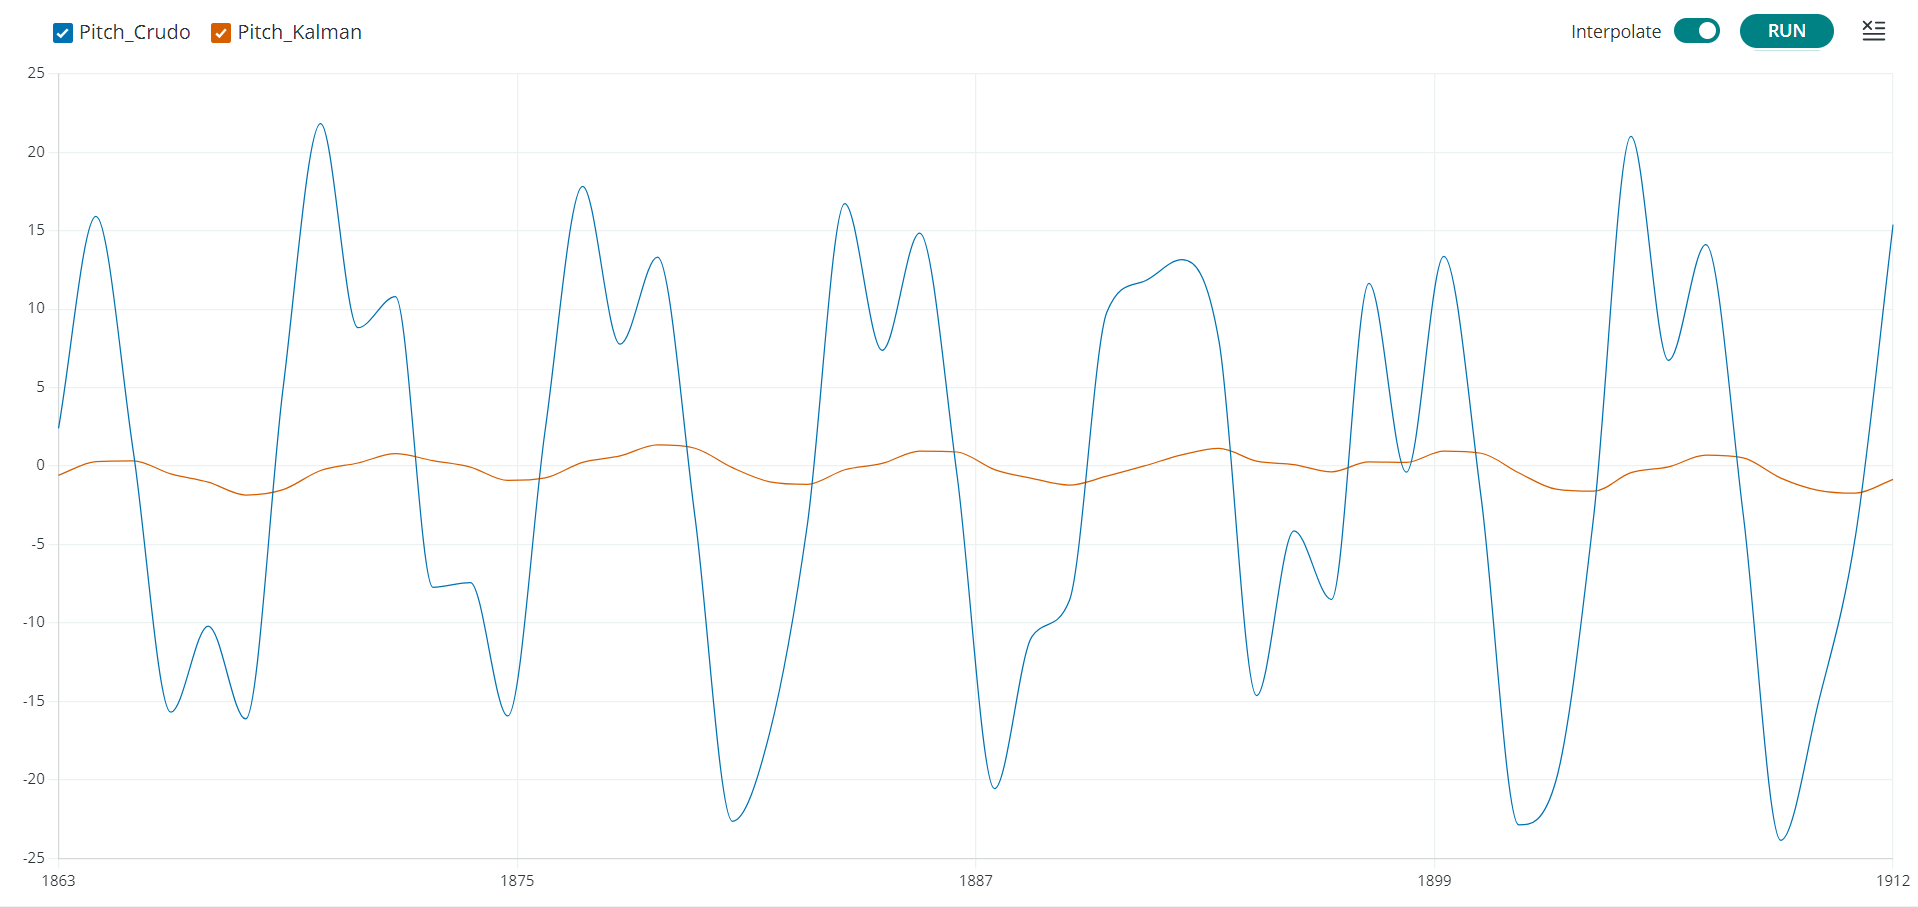
\includegraphics[width=0.45\textwidth]{Pitch_Ruido_Con_Movimiento.png}}
 \caption{Medición de \textit{pitch}.}
 \label{f:Ruido_Pitch}
\end{figure}

y para el \textit{roll} se observa:

\begin{figure}[H]
 \centering
  \subfigure[\textit{Roll} sin movimiento]{
    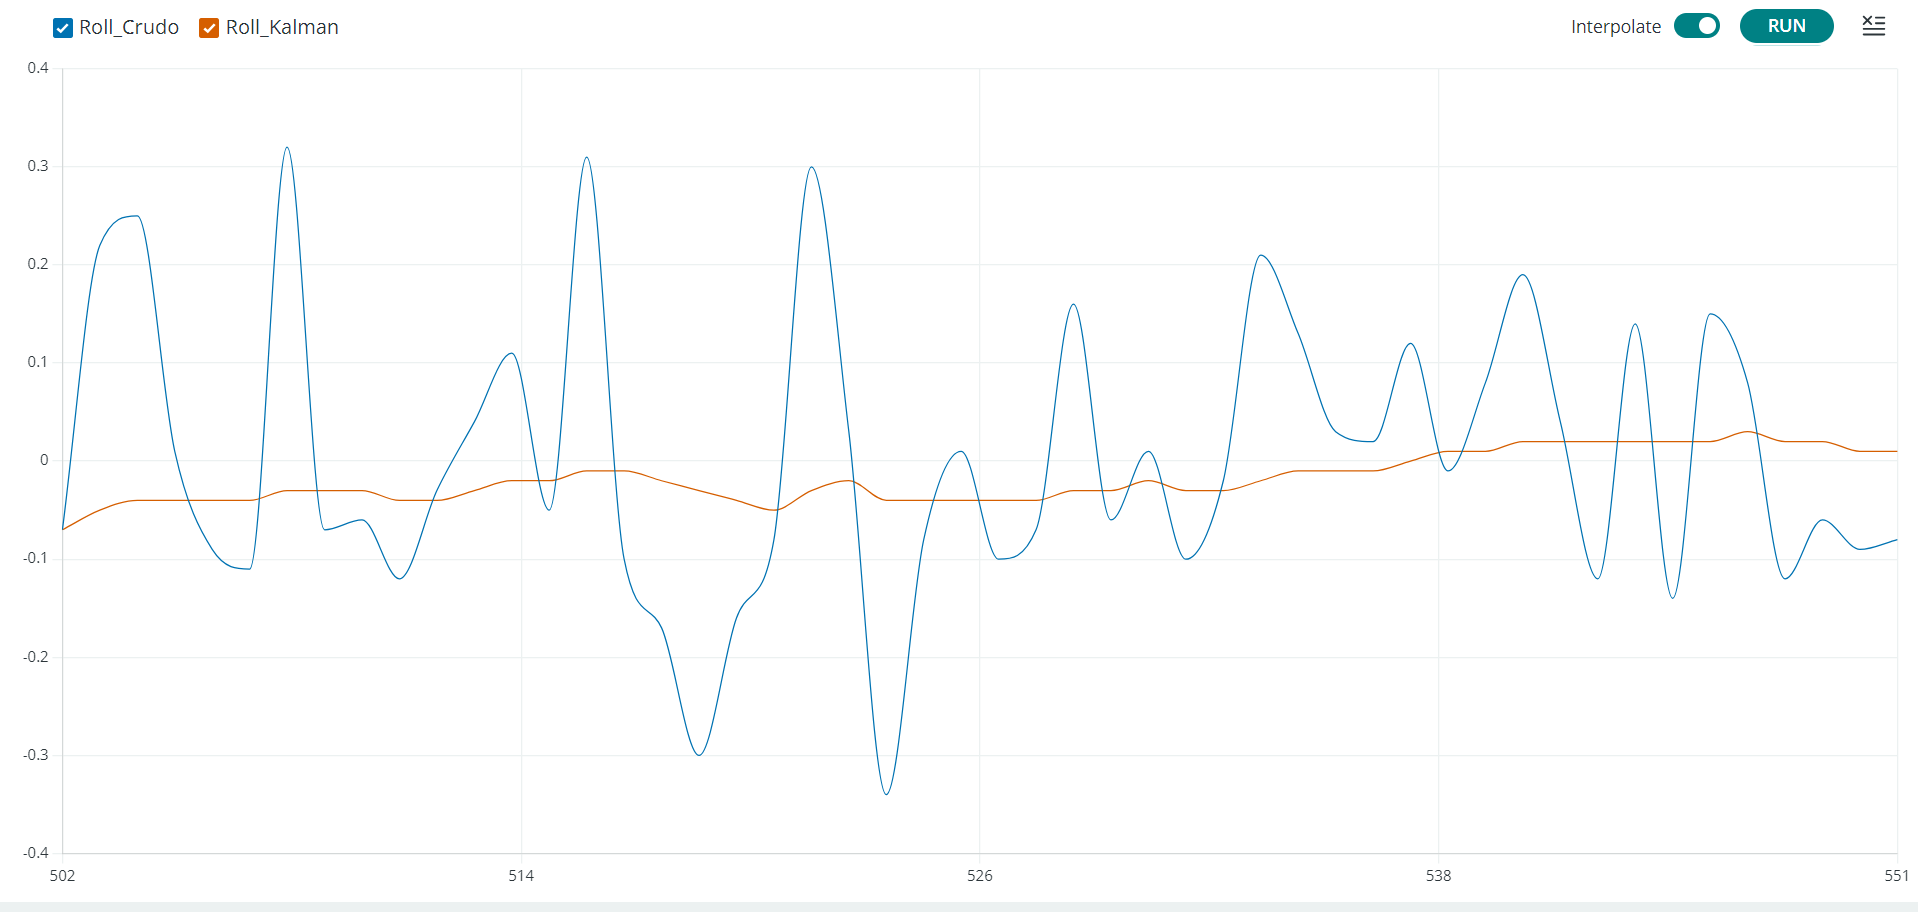
\includegraphics[width=0.45\textwidth]{Roll_Ruido_Sin_Movimiento.png}}
  \subfigure[\textit{Roll} con movimiento]{
    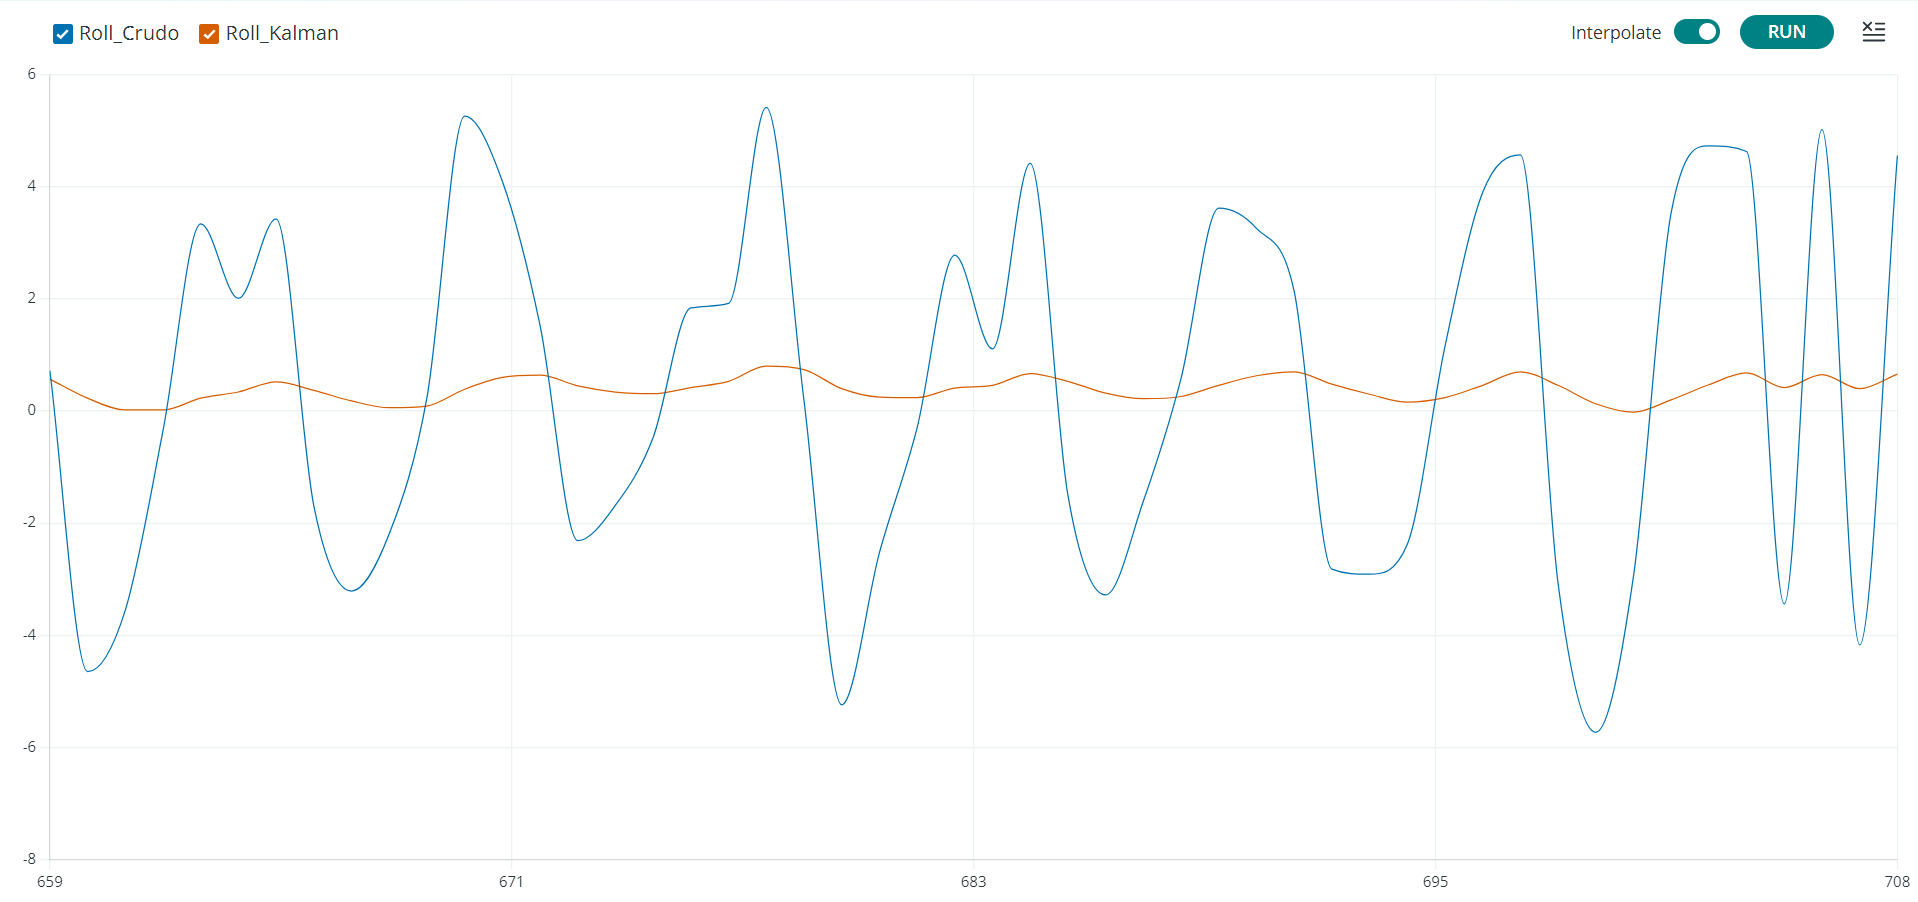
\includegraphics[width=0.45\textwidth]{Roll_Ruido_Con_Movimiento.png}}
 \caption{Medición de \textit{roll}.}
 \label{f:Ruido_Roll}
\end{figure}

Luego se analizó el comportamiento de los potenciómetros, comparando los datos leídos en crudo con los filtrados:

\begin{figure}[H]
 \centering
  \subfigure[Cambio lento]{
    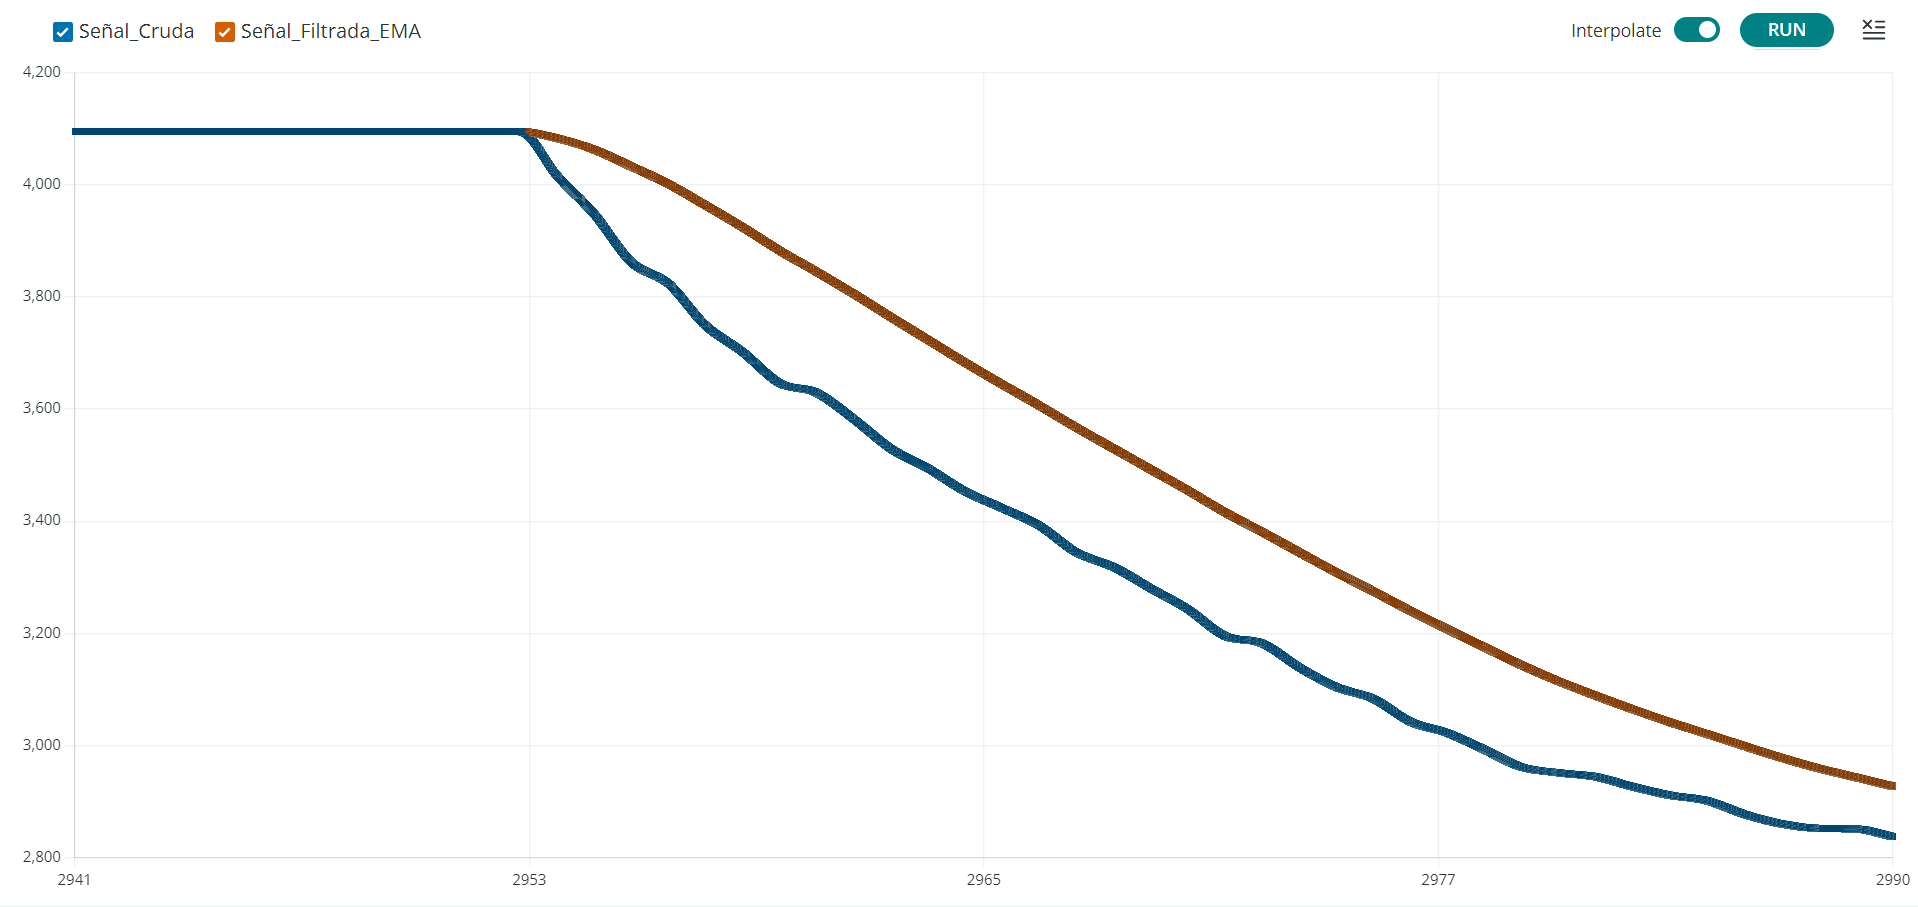
\includegraphics[width=0.45\textwidth]{Pote_Ruido.png}}
  \subfigure[Cambio brusco]{
    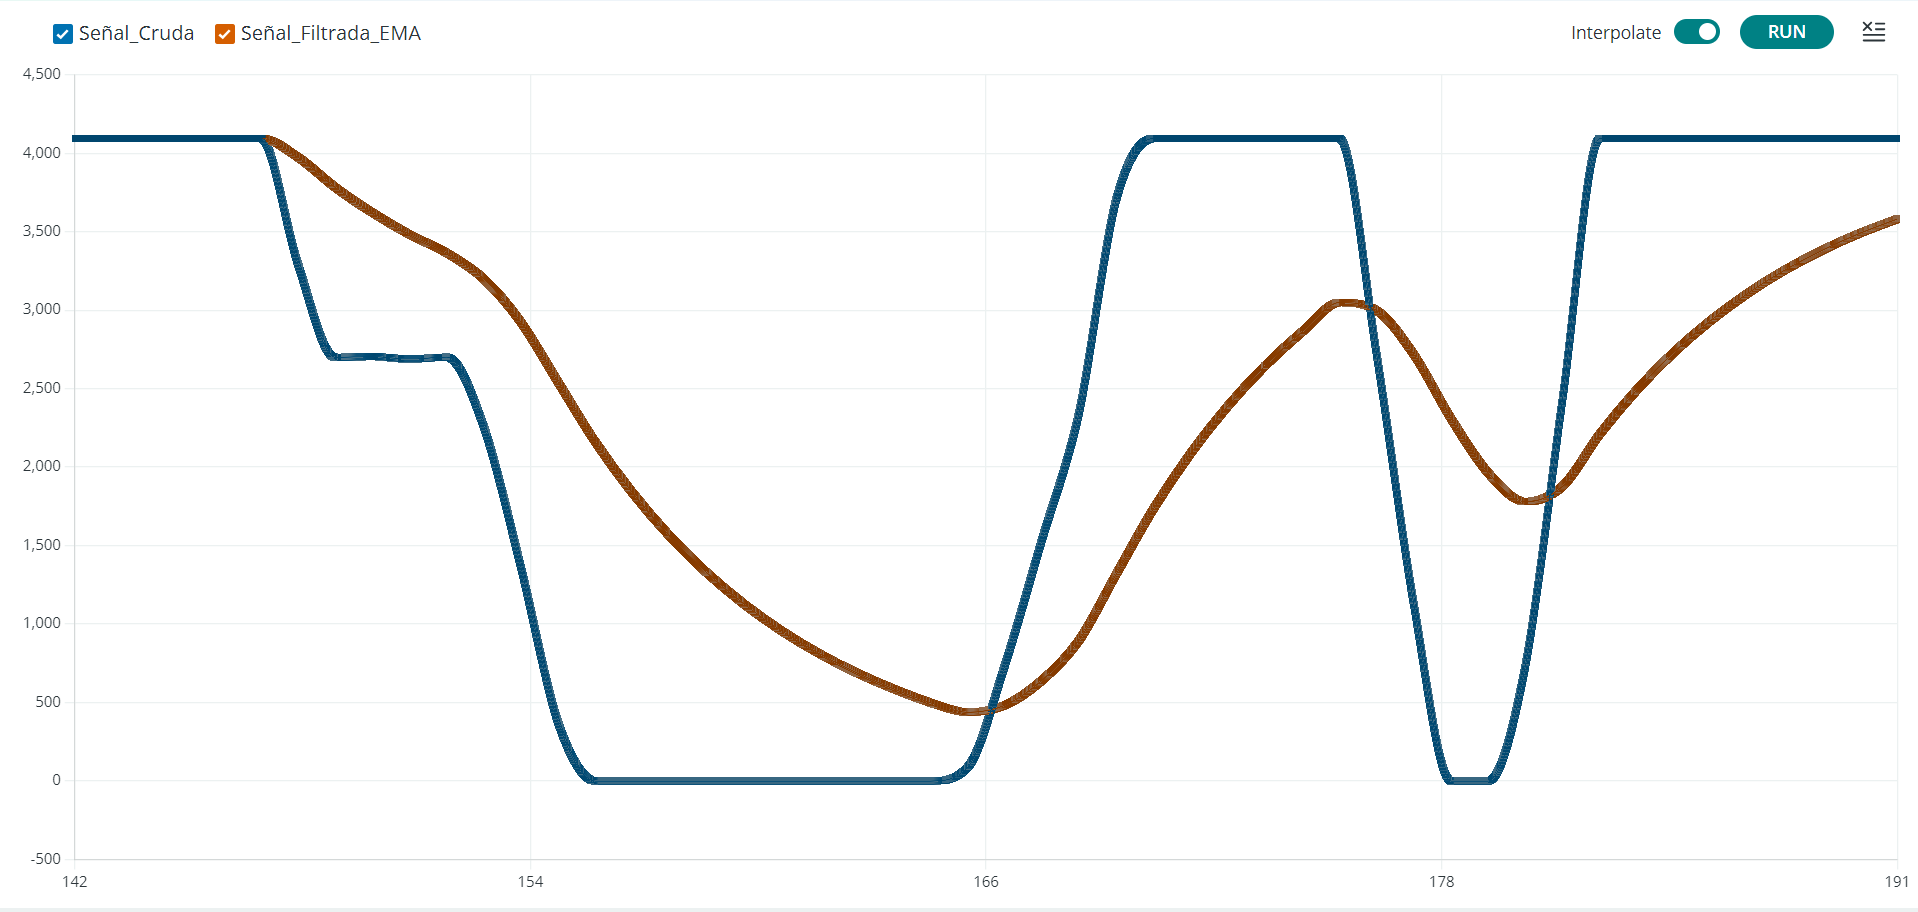
\includegraphics[width=0.45\textwidth]{Pote_Ruido_1.png}}
 \caption{Respuesta de un potenciómetro.}
 \label{f:Ruido_Potenciometros}
\end{figure}

Con el filtrado, la respuesta de la lectura es más lenta. En la versión preliminar esto se consideró deseable para proteger el mecanismo; sin embargo, sumado al filtro del receptor, el retardo resultó perceptible, lo que motivó los cambios descriptos en la sección~\ref{sec:evolucion}.

A continuación se observa la respuesta del sistema completo, transmisor y receptor:

\begin{figure}[H]
 \centering
  \subfigure[Desplazamiento vertical]{
    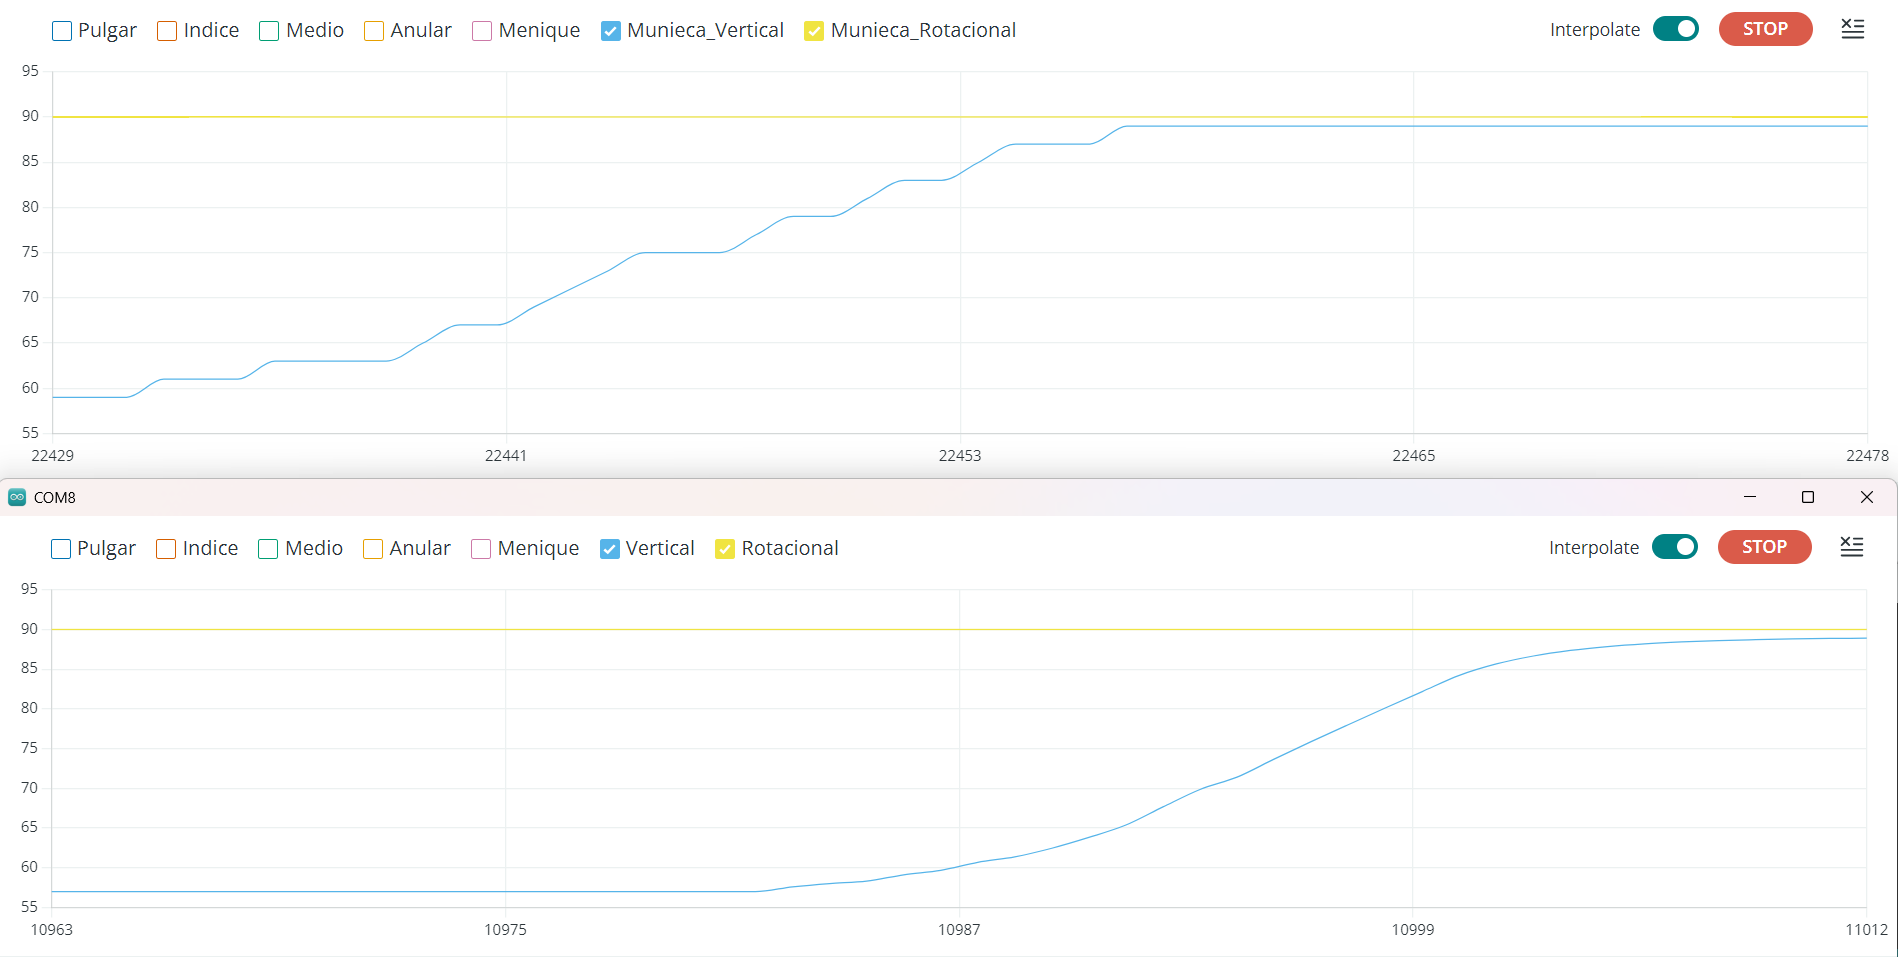
\includegraphics[width=0.47\textwidth]{Transmicion_1.png}}
  \subfigure[Rotación]{
    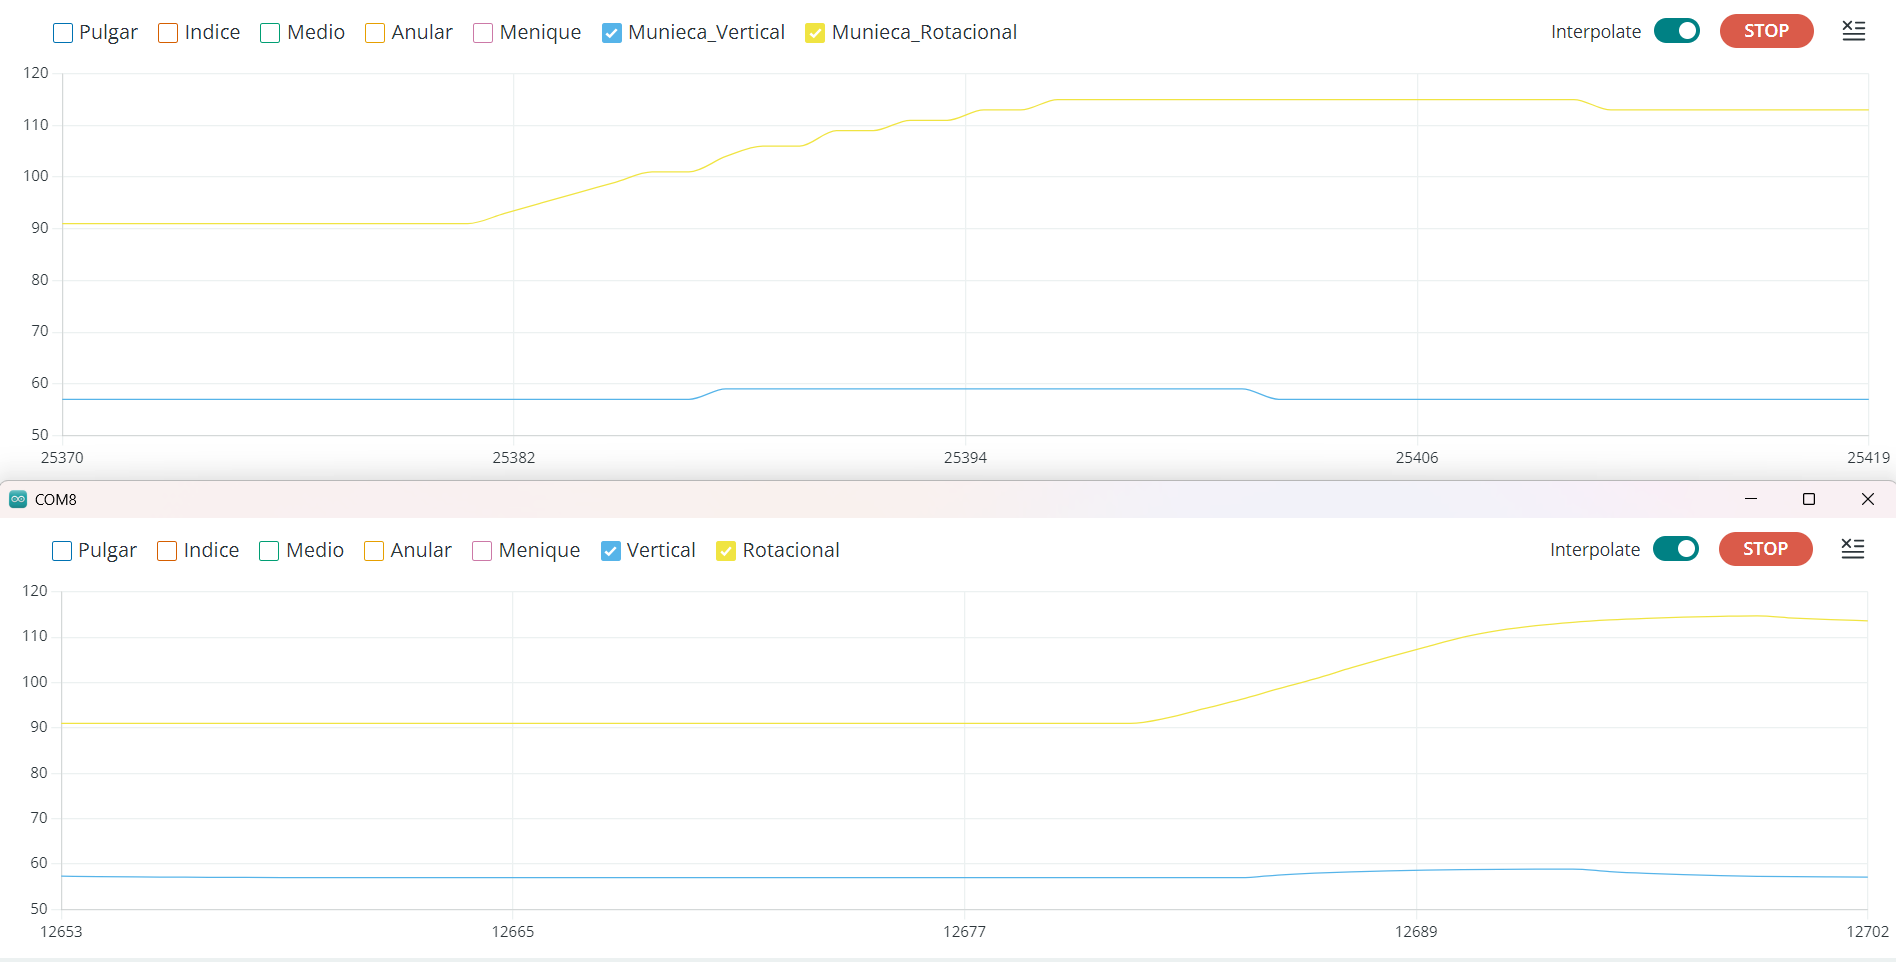
\includegraphics[width=0.47\textwidth]{Transmicion_2.png}}
  \subfigure[Subir dedo]{
    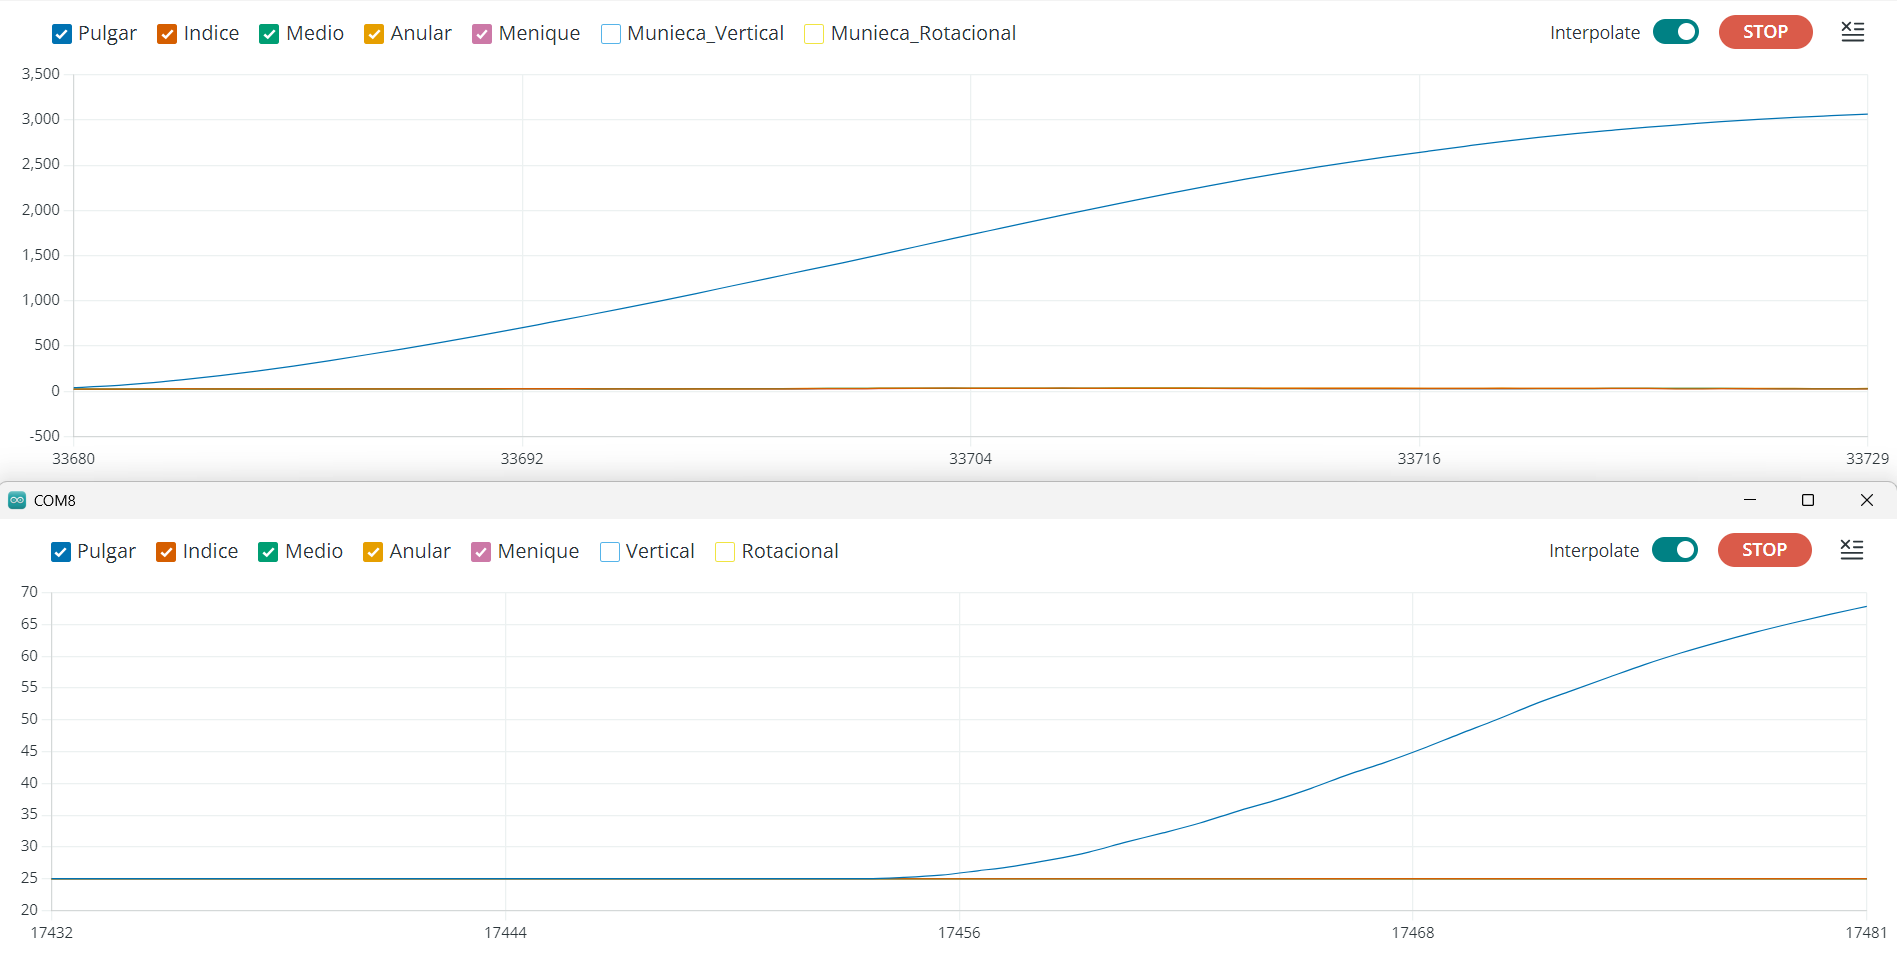
\includegraphics[width=0.47\textwidth]{Transmicion_3.png}}
  \subfigure[Bajar dedo]{
    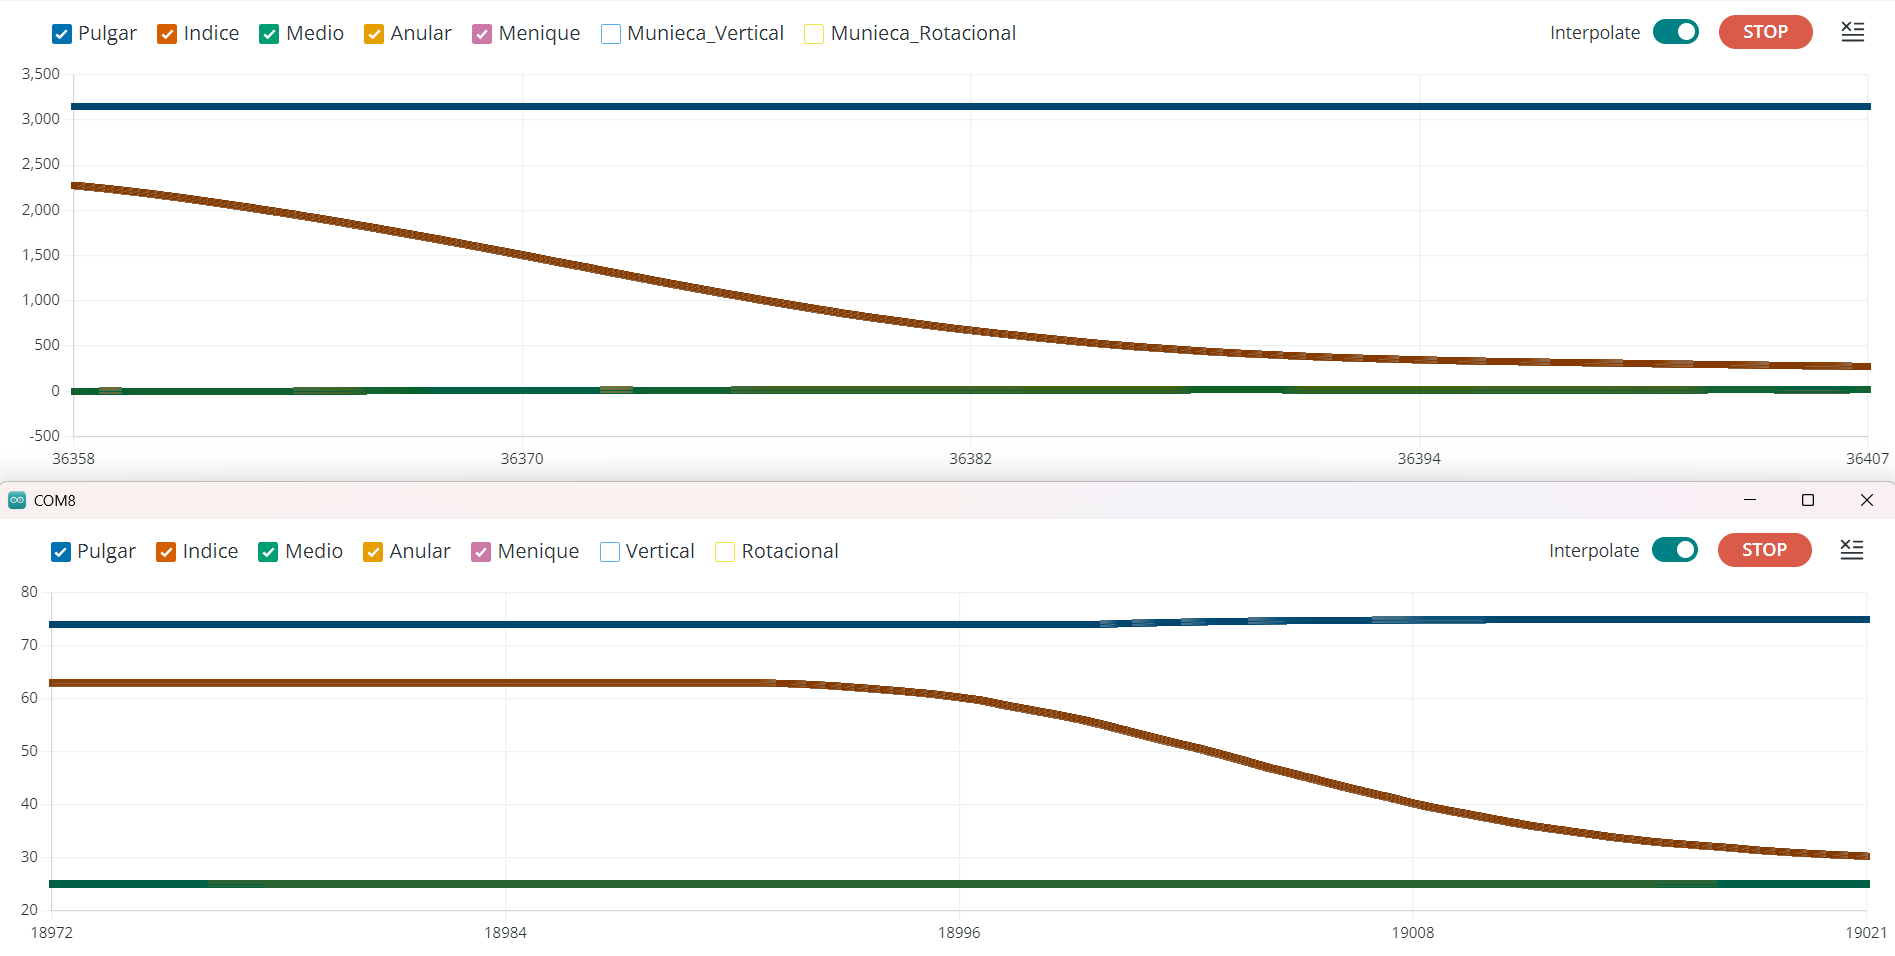
\includegraphics[width=0.47\textwidth]{Transmicion_4.png}}
 \caption{Respuesta del sistema.}
 \label{f:Respuesta_Sistema}
\end{figure}

Se observa un pequeño retardo entre la lectura en el transmisor y la réplica en el receptor. Estas curvas no permiten cuantificarlo: la telemetría se enviaba a \SI{5}{\hertz} por USB, con una resolución de \SI{200}{\milli\second}, y la hora de cada muestra la asignaba la computadora. La estimación del retardo se presenta en la sección~\ref{sec:latencia}.

\subsection{Respuesta del sistema (versión 2.3.0)}
\label{sec:pruebas_respuesta}

Para comparar la orden del guante con la posición que aplica la mano se compiló el firmware 2.3.0 de ambos nodos con una telemetría opcional en formato CSV a \SI{50}{\hertz}. En cada paquete, el transmisor imprime por USB su número de secuencia y los siete ángulos enviados; el receptor imprime el número de secuencia del paquete procesado y los siete ángulos que escribió en los servos, junto con su propio \texttt{millis()}. Un programa en MATLAB lee los dos puertos serie a la vez y, cuando llega una línea del receptor, busca la línea del transmisor con el mismo número de secuencia y la ubica en el instante del reloj del receptor en que ese paquete fue procesado. De este modo ambas curvas quedan en la misma base de tiempo sin depender de la hora en que la computadora recibe cada línea.

Por esa misma razón, el corrimiento entre las curvas no representa la latencia del enlace inalámbrico (que no se mide con este método, ya que ambas curvas se ubican al procesar el paquete en el receptor), sino el efecto del limitador de velocidad y de la banda muerta del receptor (sección~\ref{sec:slew}). Las figuras~\ref{fig:respuesta_dedos} y~\ref{fig:respuesta_muneca} muestran, para cada señal, la orden del transmisor (arriba) y la posición aplicada por el receptor (abajo). El eje de tiempo de las capturas está en milisegundos del receptor multiplicados por $10^5$ (el factor de escala que agrega MATLAB quedó fuera de las capturas): cada división corresponde a \SI{500}{\milli\second} y la ventana completa a unos \SI{5}{\second}.

\begin{figure}[H]
 \centering
  \subfigure[Pulgar]{
    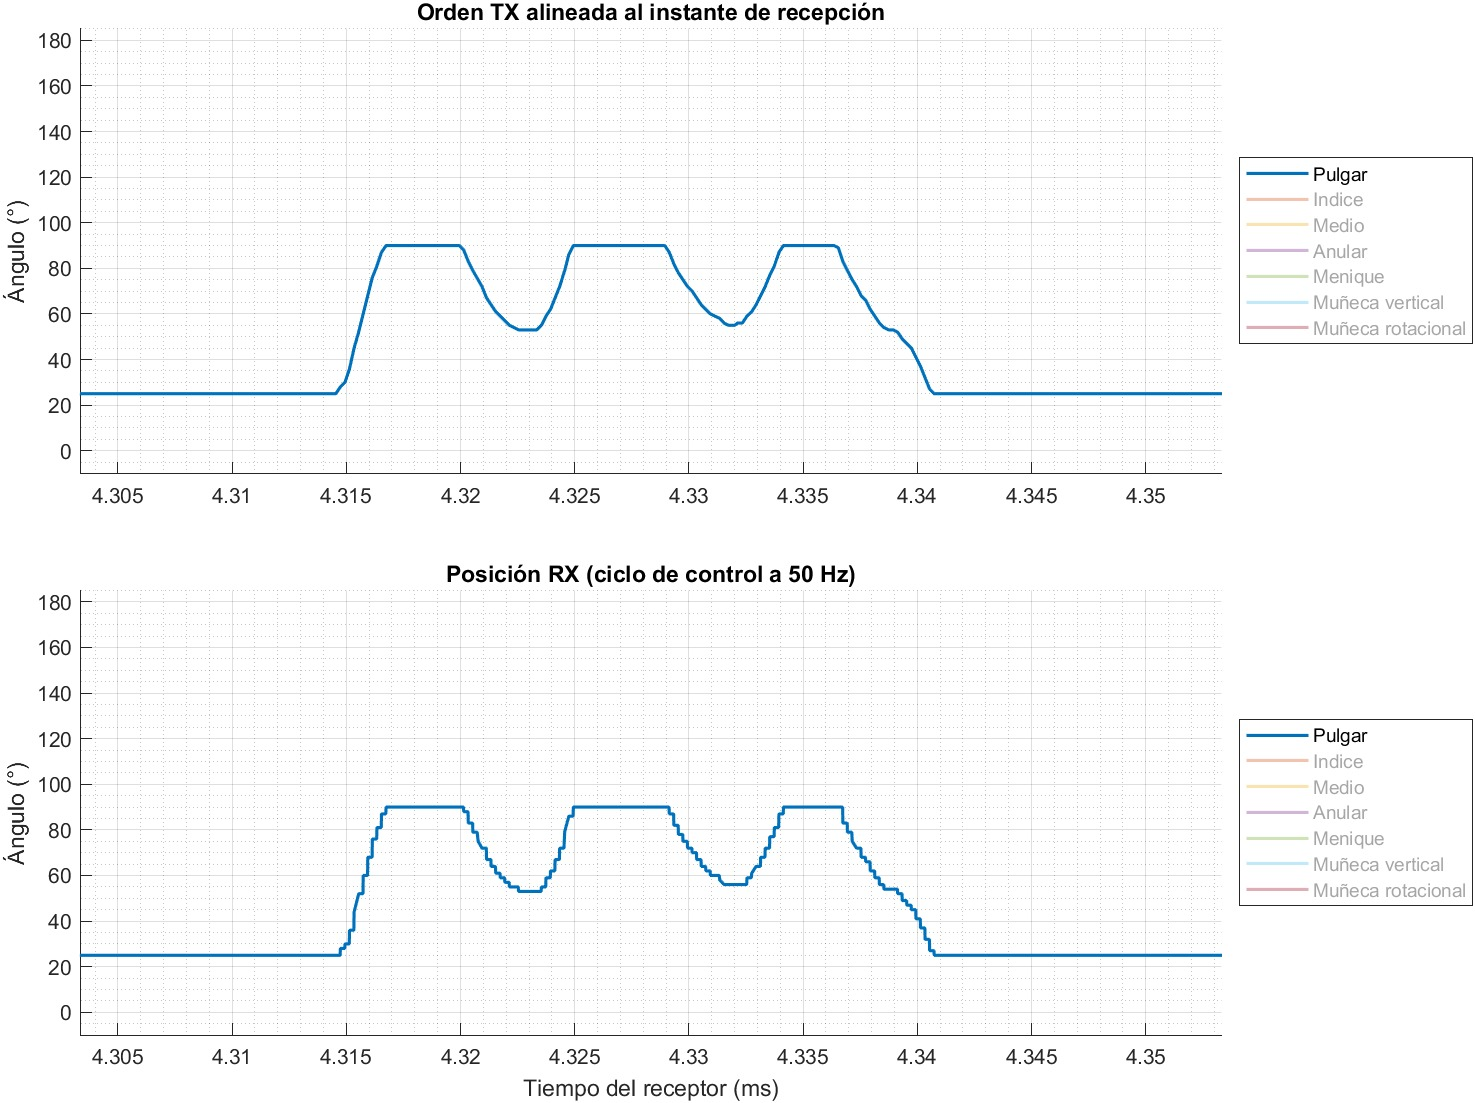
\includegraphics[width=0.48\textwidth]{Mediciones/P16_matlab_pulgar.jpg}}
  \subfigure[Índice]{
    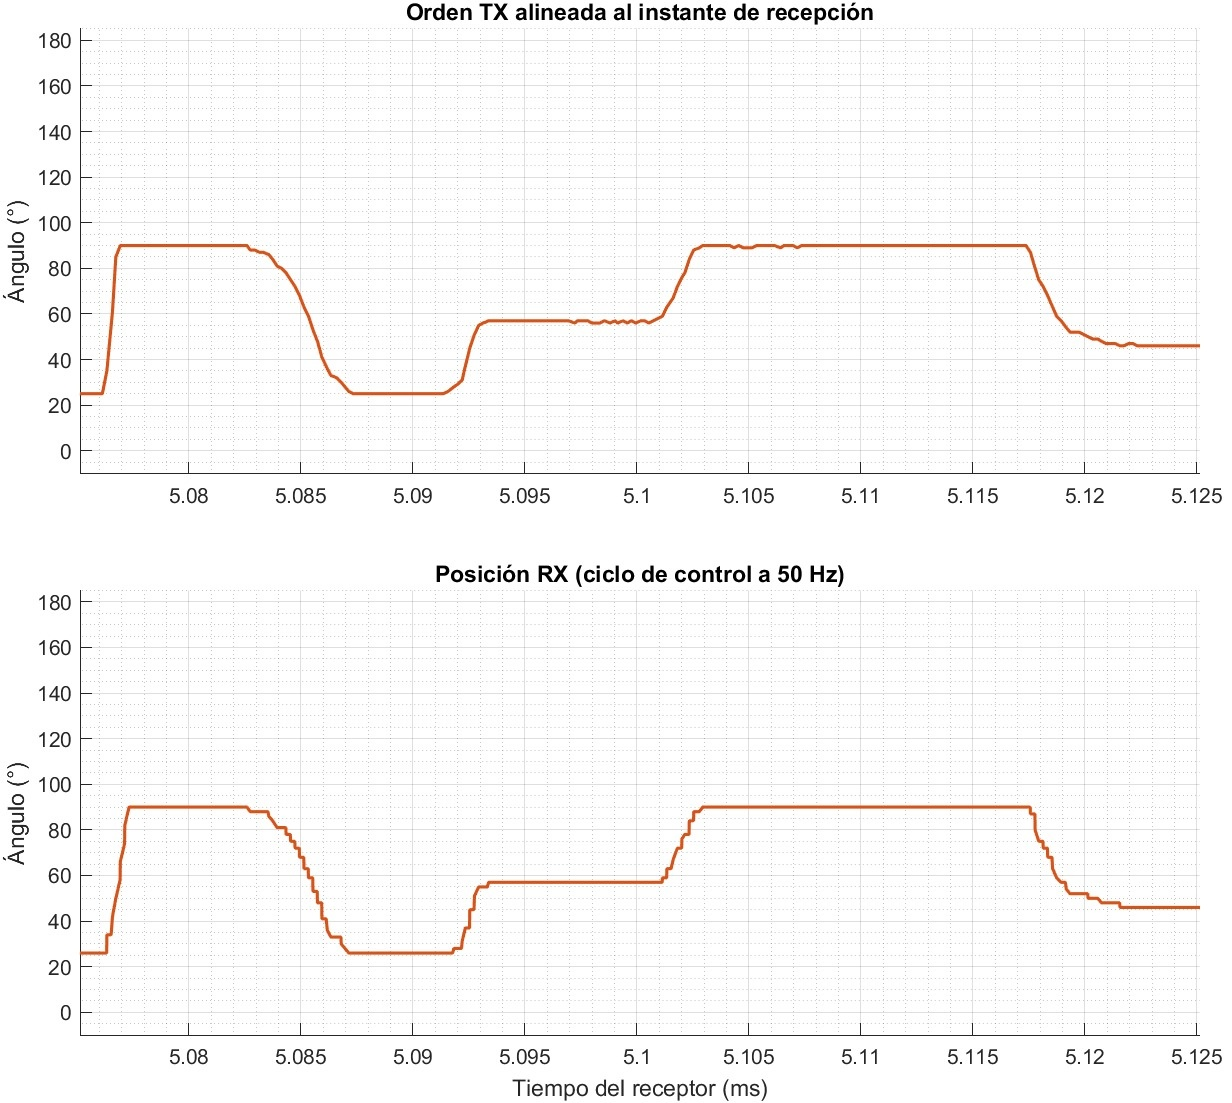
\includegraphics[width=0.48\textwidth]{Mediciones/P16_matlab_indice.jpg}}
 \caption{Respuesta de los dedos: orden del transmisor alineada por número de secuencia (arriba) y posición aplicada por el receptor (abajo).}
 \label{fig:respuesta_dedos}
\end{figure}

\begin{figure}[H]
 \centering
  \subfigure[Muñeca rotacional]{
    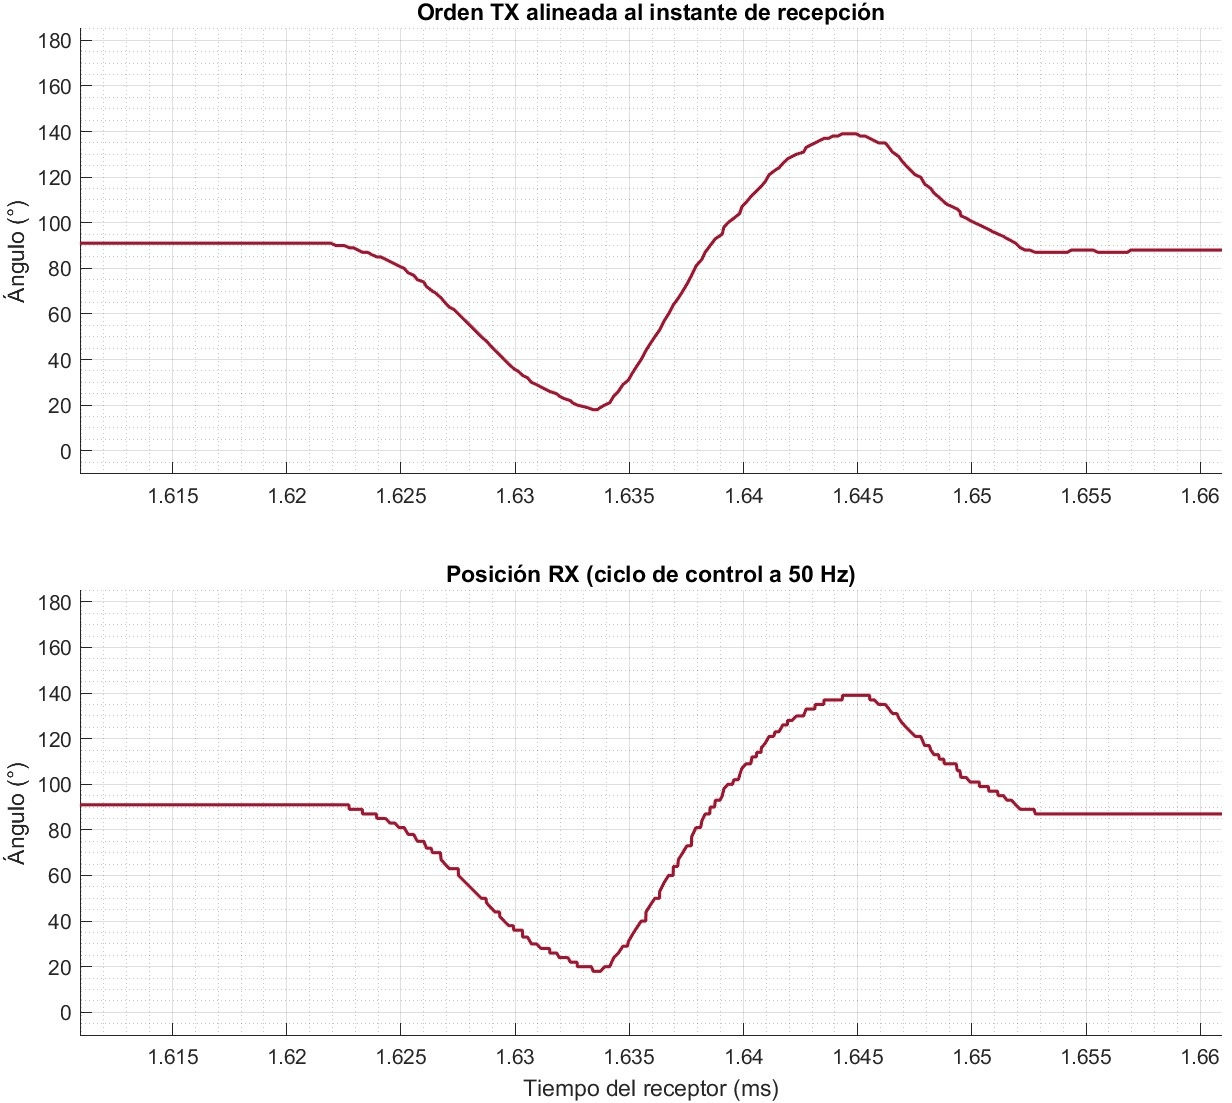
\includegraphics[width=0.48\textwidth]{Mediciones/P16_matlab_muneca_rotacional.jpg}}
  \subfigure[Muñeca vertical]{
    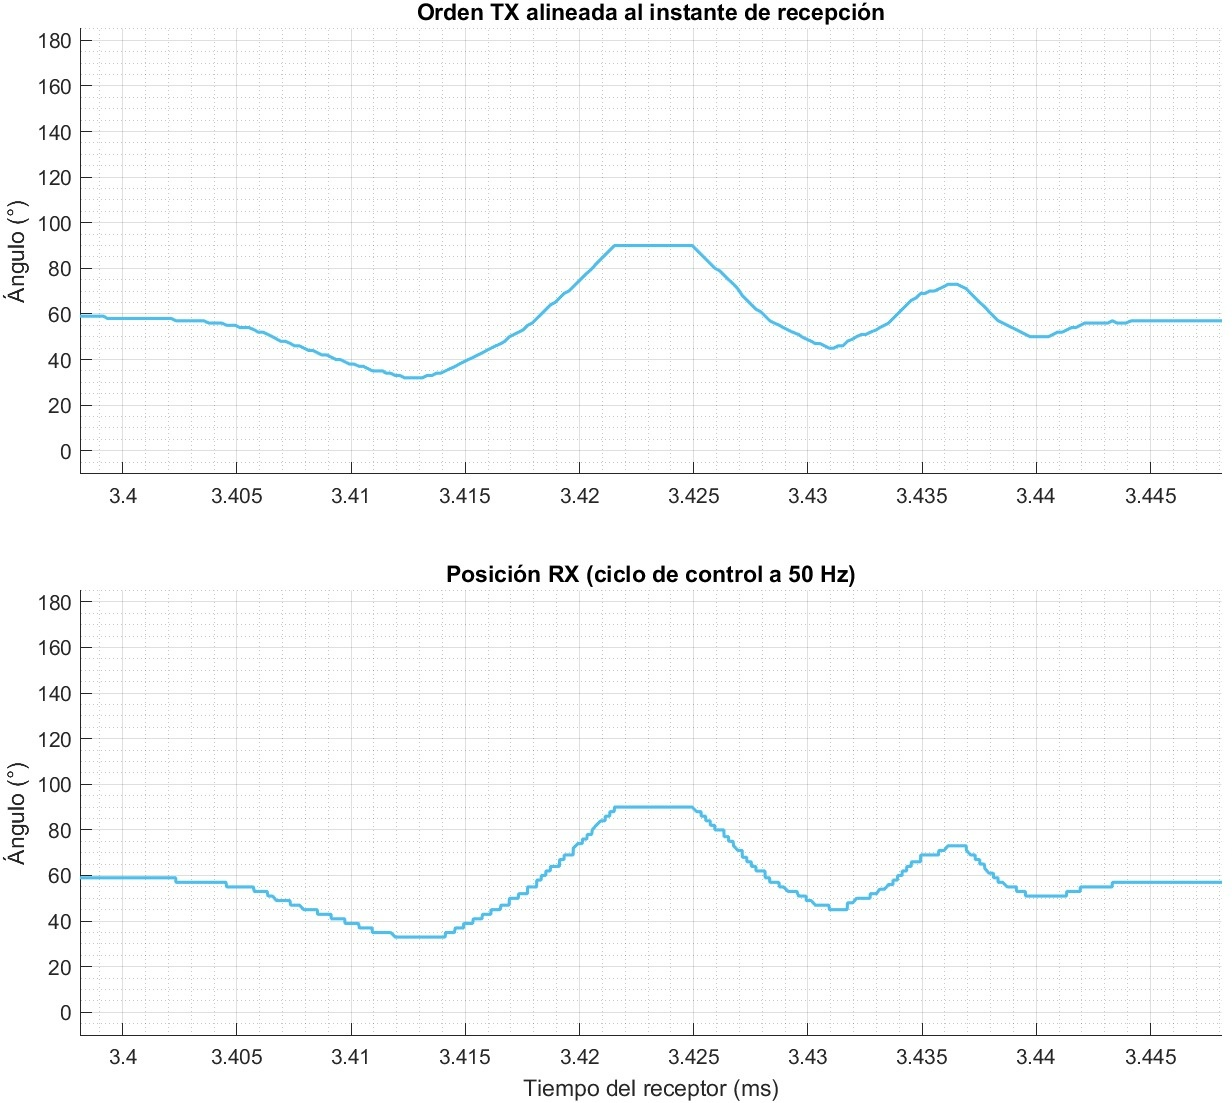
\includegraphics[width=0.48\textwidth]{Mediciones/P16_matlab_muneca_vertical.jpg}}
 \caption{Respuesta de la muñeca: orden del transmisor alineada por número de secuencia (arriba) y posición aplicada por el receptor (abajo).}
 \label{fig:respuesta_muneca}
\end{figure}

De las capturas se observa lo siguiente:

\begin{itemize}
    \item \textbf{Seguimiento.} En las cuatro señales la posición del receptor reproduce la forma de la orden, tanto en los movimientos completos (el pulgar entre \SI{25}{\degree} y \SI{90}{\degree}, la rotación de la muñeca entre \SI{18}{\degree} y \SI{139}{\degree}) como en las posiciones intermedias (el índice detenido en unos \SI{57}{\degree} y \SI{46}{\degree}). A la escala de las capturas no se distingue un retraso entre ambas curvas.
    \item \textbf{Saturación en los límites.} Las órdenes de los dedos se recortan en \SIrange{25}{90}{\degree} y la de la muñeca vertical en \SI{90}{\degree}, y el receptor se mantiene dentro de esos rangos.
    \item \textbf{Escalonamiento.} La posición del receptor se grafica en escalones, uno por ciclo de control: en cada paquete el servo recibe una nueva posición, que el limitador de velocidad acota a \SI{8}{\degree} por ciclo en los dedos y a \SIrange{4}{5}{\degree} en la muñeca. En los movimientos registrados los pasos de la orden son, en general, menores que esos límites, por lo que el receptor la sigue paquete a paquete.
    \item \textbf{Banda muerta.} Las pequeñas variaciones de \SI{1}{\degree} de la orden durante las mesetas (por ejemplo, el índice en \SI{90}{\degree} y en \SI{57}{\degree}, o la rotación de la muñeca al volver a \SI{88}{\degree}) no se trasladan al receptor, que queda quieto. Como contrapartida, la posición final puede quedar hasta \SI{1}{\degree} corrida respecto de la orden (el índice en reposo queda en \SI{26}{\degree} con una orden de \SI{25}{\degree}).
\end{itemize}

\subsection{Alimentación del receptor (versión 2.3.0)}
\label{sec:pruebas_alimentacion}

La corriente que toma el receptor de la fuente de \SI{12}{\volt} se midió con un osciloscopio Teledyne LeCroy sobre una resistencia de \SI{0.5}{\ohm} intercalada en el cable negativo de la fuente, entre el borne negativo y la entrada IN$-$ del regulador. La masa de la punta se conectó a IN$-$, que es el GND del sistema, por lo que la corriente es $I_{12} = -V/\SI{0.5}{\ohm}$; en algunas capturas el canal se invirtió y la corriente queda positiva ($I_{12} = 2\,V$). La tensión de salida del regulador se midió directamente sobre la línea de \SI{5}{\volt} de los servos.

Los valores \textit{mean}, \textit{min} y \textit{max} que muestra el osciloscopio bajo cada medición son estadísticas acumuladas de varias adquisiciones, no sólo de la captura mostrada; por eso se toman como referencia los valores de la fila \textit{value}. Las capturas originales y sus notas se encuentran en \texttt{docs/\allowbreak pruebas/\allowbreak evidencia/\allowbreak 2026-10-15} del repositorio.

\paragraph{Reposo y capacitor de entrada.} Con la mano quieta, la corriente de entrada no es continua sino una sucesión de pulsos de unos \SI{0.3}{\milli\second} cada \SIrange{0.8}{1}{\milli\second} (figura~\ref{fig:reposo_cap}a). El período varía levemente y los pulsos se espacian al desconectar los servos y desaparecen con más carga, lo que es compatible con el modo de ráfaga (\textit{pulse-skipping}) con el que los reguladores de este tipo mantienen la eficiencia con poca carga. Es un funcionamiento normal y no una falla. Al agregar el par de capacitores en la entrada del regulador (figura~\ref{fig:reposo_cap}b), el pico de corriente que ve la fuente se reduce a la mitad, de \SI{0.38}{\ampere} a \SI{0.18}{\ampere}, y la corriente adopta forma de diente de sierra. La corriente media no cambia de forma apreciable (unos \SIrange{75}{100}{\milli\ampere}): el capacitor cambia la forma de la corriente, no el consumo. Parte de este filtrado lo aporta la propia resistencia de medición, ya que $\SI{0.5}{\ohm} \times \SI{470}{\micro\farad} \approx \SI{0.24}{\milli\second}$, del orden del período de las ráfagas; sin ella, el suavizado sería algo menor.

\begin{figure}[H]
 \centering
  \subfigure[Sin capacitores de entrada]{
    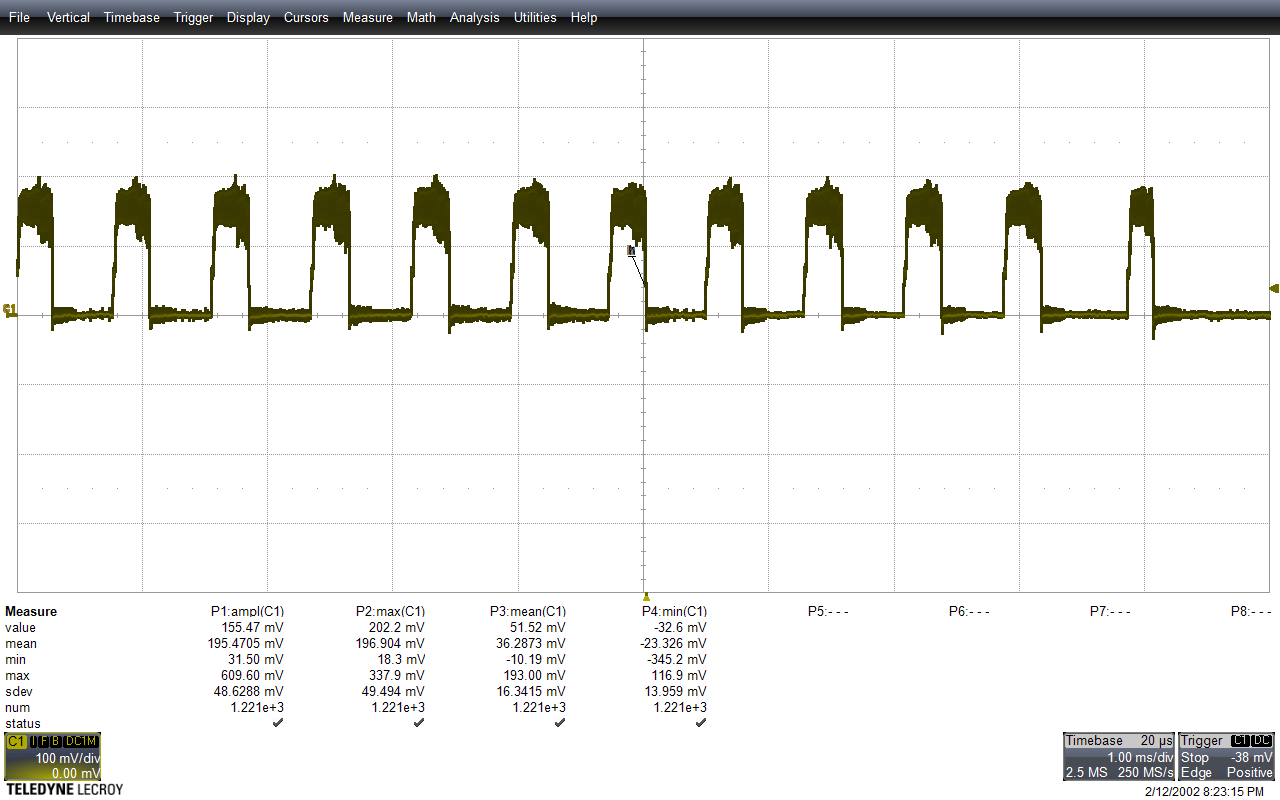
\includegraphics[width=0.47\textwidth]{Mediciones/P02_reposo_sin_cap_entrada.png}}
  \subfigure[Con capacitores de entrada]{
    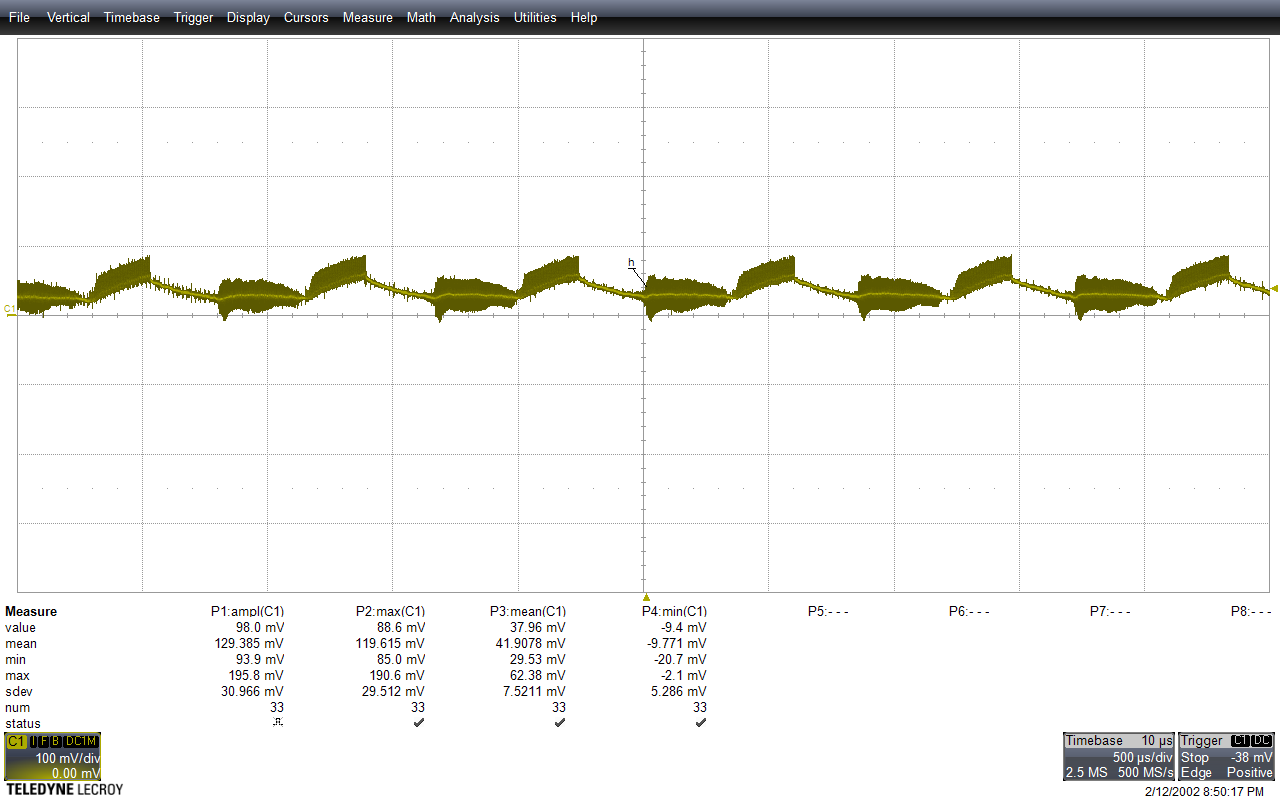
\includegraphics[width=0.47\textwidth]{Mediciones/P02_reposo_con_cap_entrada.png}}
 \caption{Corriente de entrada a \SI{12}{\volt} con la mano en reposo (canal invertido, \SI{100}{\milli\volt}/div $\equiv$ \SI{0.2}{\ampere}/div; base de tiempo de \SI{1}{\milli\second}/div y \SI{500}{\micro\second}/div).}
 \label{fig:reposo_cap}
\end{figure}

\paragraph{Movimiento y servo bloqueado.} Al mover la muñeca en sus dos ejes a la vez (figura~\ref{fig:carga}a), la corriente media en la ventana de \SI{10}{\milli\second} de la captura es de unos \SI{0.21}{\ampere}, con picos de \SI{0.6}{\ampere}; el máximo registrado entre todas las adquisiciones fue de unos \SI{0.72}{\ampere}. Al bloquear a mano un servo (figura~\ref{fig:carga}b), la corriente se mantiene en unos \SIrange{0.55}{0.6}{\ampere} y el regulador conmuta en forma continua. El corte de la corriente de unos \SI{0.4}{\milli\second} al final de esa captura corresponde al instante en que se soltó el servo: deja de exigir corriente y el regulador deja de conmutar por un momento, hasta volver al régimen de reposo. No es una falla.

\begin{figure}[H]
 \centering
  \subfigure[\textit{Pitch} y \textit{roll} simultáneos (canal invertido, \SI{100}{\milli\volt}/div $\equiv$ \SI{0.2}{\ampere}/div)]{
    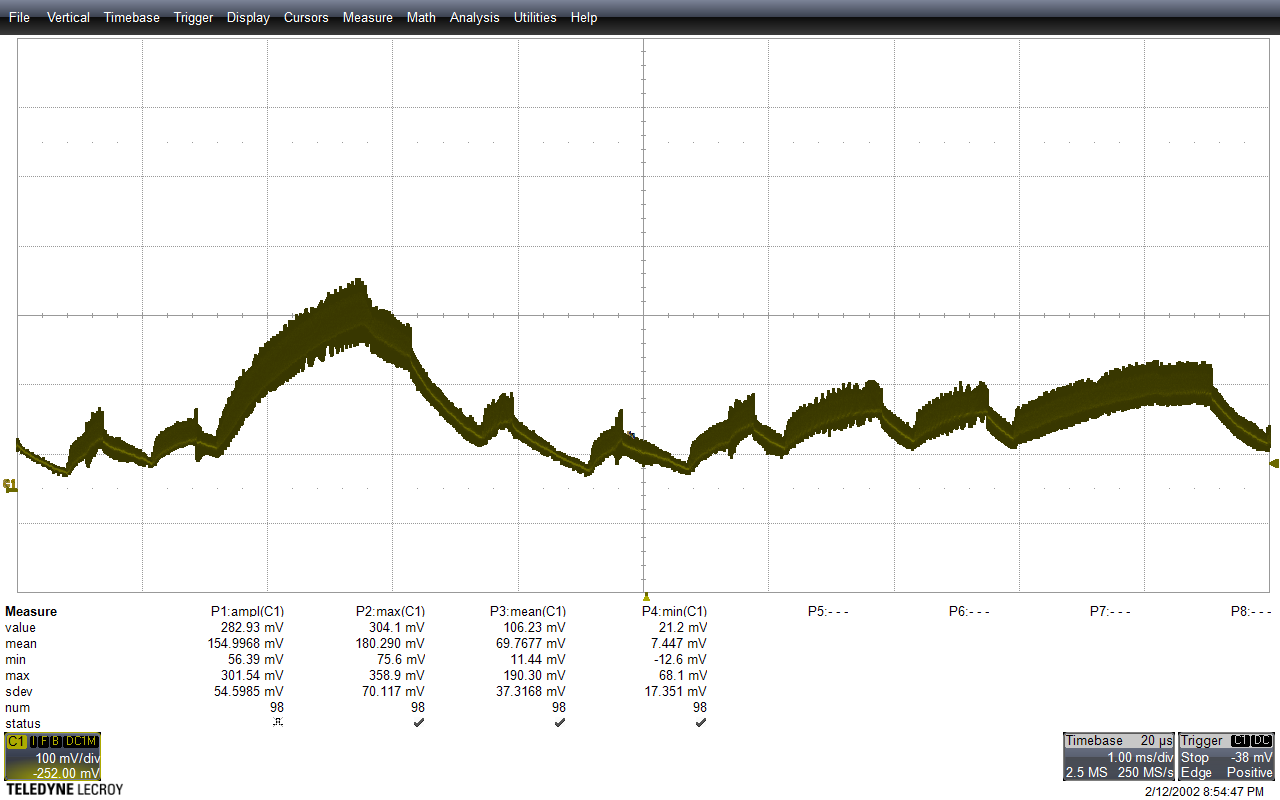
\includegraphics[width=0.47\textwidth]{Mediciones/P03_pitch_roll_con_cap.png}}
  \subfigure[Servo bloqueado (\SI{200}{\milli\volt}/div $\equiv$ \SI{0.4}{\ampere}/div)]{
    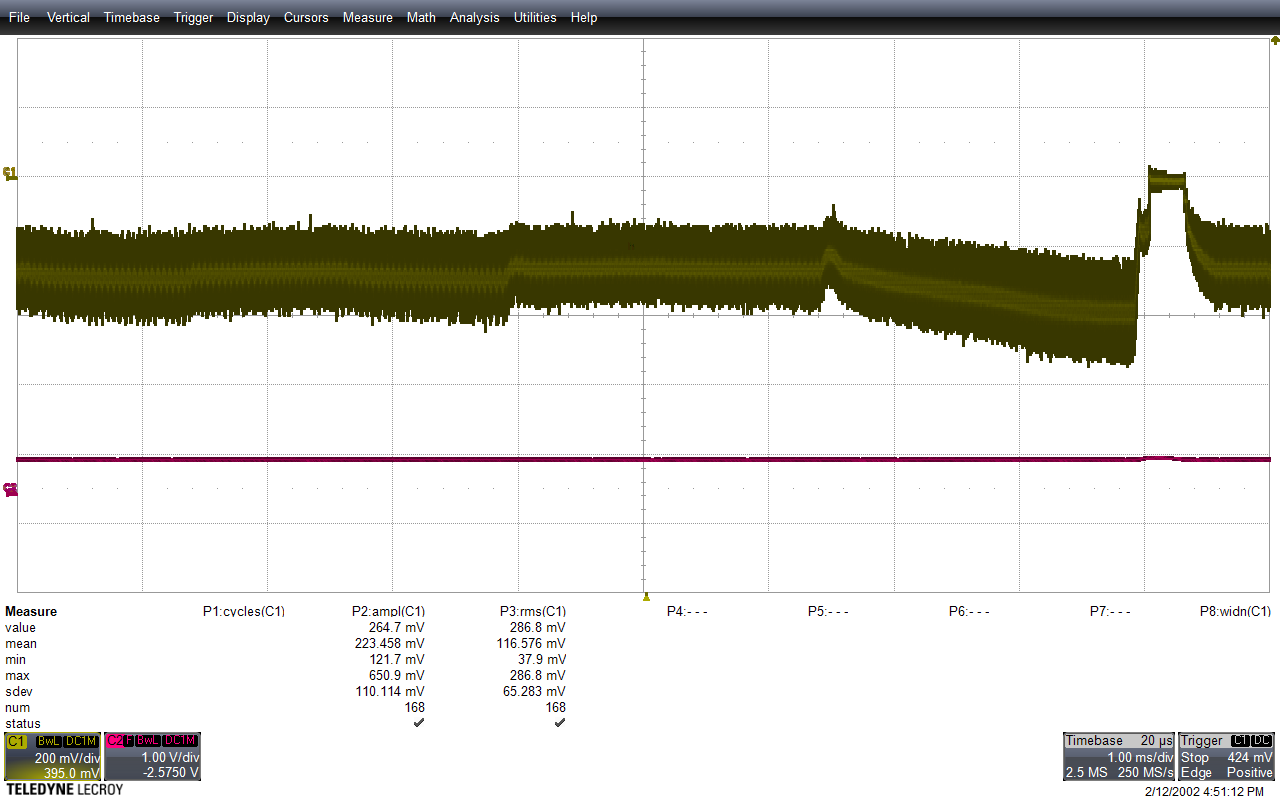
\includegraphics[width=0.47\textwidth]{Mediciones/P03_servo_bloqueado.png}}
 \caption{Corriente de entrada a \SI{12}{\volt} con carga (\SI{1}{\milli\second}/div).}
 \label{fig:carga}
\end{figure}

\paragraph{Tensión de salida.} El valor eficaz de la línea de \SI{5}{\volt} de los servos se mantuvo entre \SI{5.14}{\volt} y \SI{5.25}{\volt} en 57 adquisiciones, con un desvío de \SI{16}{\milli\volt} (figura~\ref{fig:v5}). En la traza se ven ondulaciones breves de algunas décimas de volt; con la escala de \SI{1}{\volt}/div utilizada no es posible resolver el rizado con más detalle, y el parámetro de amplitud del osciloscopio no es confiable en esas condiciones, por lo que se toma como referencia el valor eficaz.

\begin{figure}[H]
    \centering
    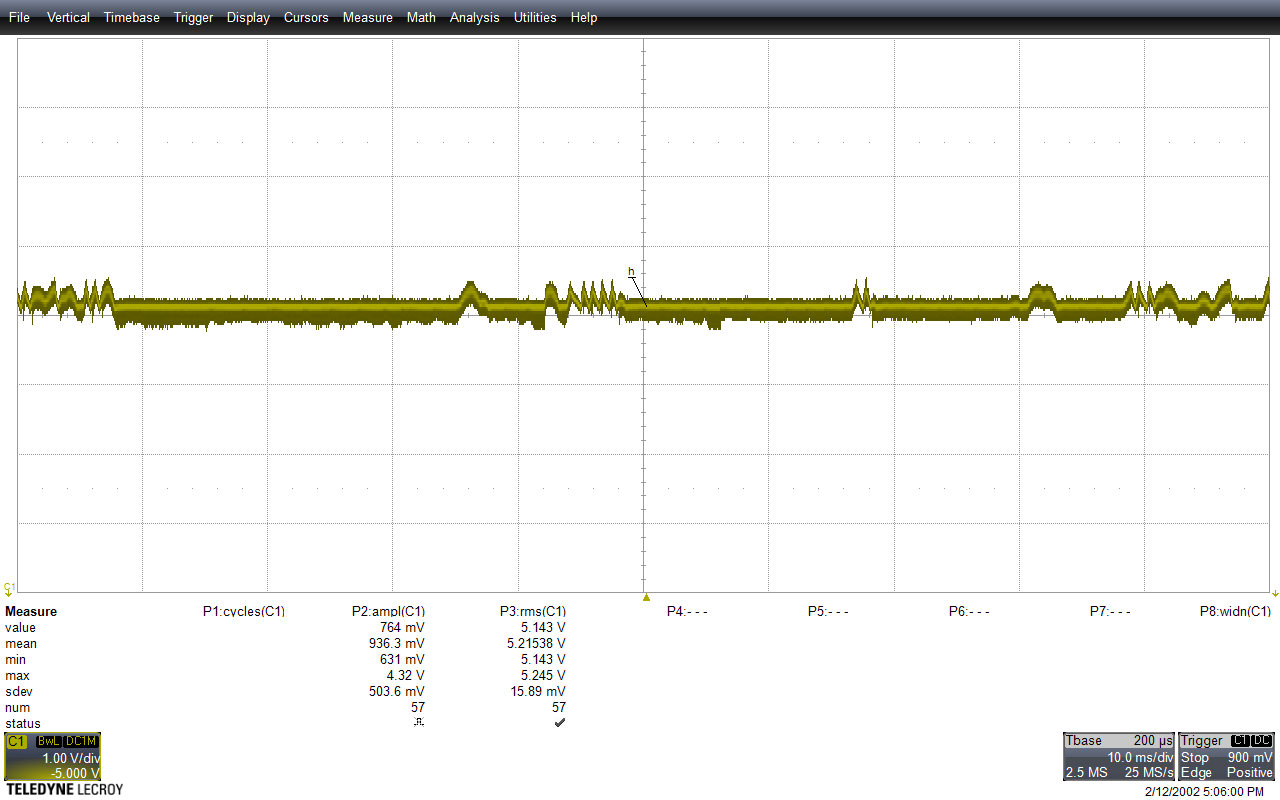
\includegraphics[width=0.7\textwidth]{Mediciones/P02_V5_regulador.png}
    \caption{Tensión de salida del regulador (\SI{1}{\volt}/div, \SI{10}{\milli\second}/div, límite de ancho de banda activado).}
    \label{fig:v5}
\end{figure}

\paragraph{Conclusiones de las mediciones.} El consumo del receptor queda muy por debajo de la capacidad de la fuente (\SI{4}{\ampere}) y del regulador (\SI{3}{\ampere} a la salida): aun en el peor caso registrado, la corriente de entrada no superó los \SI{0.75}{\ampere} a \SI{12}{\volt}. Los picos de bloqueo de los MG946R estimados en la sección~\ref{sec:alimentacion} con las hojas de datos no se presentaron en el uso normal, lo que es coherente con la acción del limitador de velocidad, aunque no se midió el consumo sin él. La línea de \SI{5}{\volt} también se observó con la mano en movimiento y su valor casi no varió, por lo que los picos de corriente no comprometen la alimentación de los servos. No se midió la corriente media en movimiento continuo durante un tiempo prolongado.

\section{Conclusiones}
\label{sec:conclusiones}

\pendiente{Borrador: completar con la latencia medida y con las pruebas de deriva y retorno de la muñeca con la versión actual.}

Se desarrolló un sistema de telerobótica de bajo costo en el que un guante con sensores comanda una mano impresa en 3D por medio de un enlace inalámbrico ESP-NOW. El sistema replica la flexión de los cinco dedos y dos grados de libertad de la muñeca (desplazamiento vertical y rotación), con un firmware sobre FreeRTOS en cada nodo.

Los principales resultados y aprendizajes del proyecto son:

\begin{itemize}
    \item \textbf{Separación de responsabilidades.} El guante concentra la calibración y el cálculo de los ángulos, y la mano sólo valida, suaviza y mueve los servos. Así, cambiar de operador requiere recalibrar únicamente el guante.
    \item \textbf{Seguridad en el firmware.} La verificación por checksum, el modo de seguridad ante la pérdida de paquetes, los límites mecánicos y el limitador de velocidad evitan que un dato erróneo o un corte del enlace dañen la mecánica. La pausa del envío durante la calibración (versión 2.3.0) se apoya en ese mismo modo de seguridad y se verificó en hardware.
    \item \textbf{Proceso iterativo validado en hardware.} Las pruebas de la versión preliminar mostraron que el doble filtrado (en el transmisor y en el receptor) introducía un retardo perceptible y que la implementación del filtro de Kalman producía deriva en la muñeca. Su reemplazo por un filtro complementario sobre ángulos absolutos y por un limitador de velocidad en el receptor resolvió ambos problemas con un algoritmo más simple de ajustar.
    \item \textbf{Respuesta del sistema.} Con la versión 2.3.0, la posición de la mano reproduce la orden del guante en los dedos registrados (pulgar e índice) y en los dos ejes de la muñeca, incluidas las posiciones intermedias; la banda muerta descarta las variaciones de \SI{1}{\degree} de la orden, a costa de un error final de hasta \SI{1}{\degree}.
    \item \textbf{Alimentación.} Las mediciones con la versión 2.3.0 muestran que el receptor consume a \SI{12}{\volt} entre \SIrange{75}{100}{\milli\ampere} en reposo y menos de \SI{0.75}{\ampere} en los picos registrados, muy por debajo de la capacidad de la fuente y del regulador. Separar la alimentación del ESP32 (por USB) de la de los servos evita que un pico de corriente de los motores reinicie el microcontrolador.
\end{itemize}

Entre las limitaciones del sistema actual se encuentran la falta de realimentación de fuerza al operador, la imposibilidad de medir el giro sobre el eje vertical (\textit{yaw}) con el MPU6050, que no tiene magnetómetro, y la dependencia de una calibración inicial de los dedos para cada operador. Además, la latencia de punta a punta se estimó a partir del código y de las hojas de datos, pero todavía no se midió.

\subsection{Trabajo futuro}

Durante el desarrollo se identificaron las siguientes mejoras, que no se implementaron:

\begin{itemize}
    \item \textbf{Medir la latencia real} de punta a punta (sección~\ref{sec:latencia}).
    \item \textbf{Filtro \textit{One Euro}} \cite{casiez2012} en lugar del limitador de velocidad: filtra fuertemente en reposo y casi nada durante los movimientos rápidos.
    \item \textbf{Aumentar la tasa de envío a \SI{100}{\hertz}}. El limitador de velocidad actúa por iteración, por lo que en ese caso debería escalarse con el tiempo real entre iteraciones; de lo contrario la velocidad máxima se duplicaría.
    \item \textbf{PWM de mayor frecuencia en los MG946R}, de \SIrange{100}{200}{\hertz}. El fabricante sólo especifica \SI{50}{\hertz}, por lo que debería probarse vigilando la temperatura de los servos.
    \item \textbf{Robustez de la calibración:} rechazar una calibración en la que la lectura de mano abierta y cerrada coincidan, que hoy produciría una división por cero en la conversión del dedo.
    \item \textbf{Emparejamiento sin reprogramar:} la dirección MAC del receptor está fija en el código del transmisor; si se cambia la placa receptora hay que reprogramar el guante.
    \item \textbf{Realimentación al operador}, por ejemplo háptica, para tareas de manipulación.
\end{itemize}


\newpage
\bibliographystyle{bst/IEEEtran}
\bibliography{bib/IEEEabrv,bib/IEEEreferencias}

\newpage
\begin{appendices}
\section{Guía de ajuste de parámetros}
\label{ap:ajuste}

Todas las constantes ajustables se encuentran al comienzo de cada programa. La tabla~\ref{tab:ajuste} indica qué modificar ante cada síntoma.

\begin{table}[H]
\centering
\begin{tabularx}{\textwidth}{X l l}
\toprule
\textbf{Síntoma} & \textbf{Parámetro} & \textbf{Nodo} \\
\midrule
Un dedo de la mano se mueve al revés & \texttt{INVERTIR\_DEDO[i]} & Receptor \\
Un dedo no llega a abrir o cerrar del todo & Recalibrar (comando \texttt{c}) & Transmisor \\
Movimientos bruscos o reinicios de la placa & Reducir \texttt{VEL\_MAX\_*} & Receptor \\
Movimientos lentos & Aumentar \texttt{VEL\_MAX\_*} & Receptor \\
Servos que zumban en reposo & Aumentar \texttt{DEADBAND\_*} & Receptor \\
Muñeca no centrada con la mano en reposo & \texttt{TRIM\_PITCH\_DEG}, \texttt{TRIM\_ROLL\_DEG} & Transmisor \\
Muñeca inestable por vibraciones & Aumentar \texttt{ALPHA\_COMPLEMENTARIO} o DLPF a \SI{21}{\hertz} & Transmisor \\
Muñeca que tarda en asentarse en el ángulo real & Reducir \texttt{ALPHA\_COMPLEMENTARIO} & Transmisor \\
Recorrido de la muñeca corto o excesivo & \texttt{PITCH\_MANO\_*}, \texttt{ROLL\_MANO\_MAX}, \texttt{SERVO\_V\_*} & Transmisor \\
La mano vuelve sola al reposo con el guante encendido & Revisar alcance; \texttt{TIMEOUT\_FAILSAFE\_MS} & Receptor \\
Telemetría \texttt{NO\_ACK} permanente & \texttt{macReceptor[]} & Transmisor \\
\bottomrule
\end{tabularx}
\caption{Guía de ajuste de parámetros.}
\label{tab:ajuste}
\end{table}

\section{Estructura del firmware}
\label{sec:estructura_firmware}

\subsection{Código fuente}
\label{sec:codigo_fuente}

El código completo del proyecto está disponible en un repositorio público de GitHub:

\begin{center}
\url{https://github.com/sevastianamoroso/proyecto-mano}
\end{center}

El repositorio contiene el firmware del guante (\texttt{Transmisor/}) y de la mano (\texttt{Receptor/}), el receptor modificado para la medición de latencia (\texttt{Receptor\_Latencia/}), el plan y el registro de pruebas, la documentación del firmware y las fuentes de este informe. Cada versión del firmware descrita en la sección~\ref{sec:evolucion} está marcada con una etiqueta de git (\texttt{v1.0.0} a \texttt{v2.3.0}), de modo que cualquiera de ellas puede recuperarse y volver a grabarse en los ESP32. Este apéndice describe la versión 2.3.0.

\subsection{Cómo leer los diagramas}

El firmware está escrito en C++ para Arduino, pero \textbf{no define clases propias}: está organizado en variables globales, funciones y tareas de FreeRTOS, repartidos en dos programas (\texttt{Transmisor.ino} y \texttt{Receptor.ino}) que comparten el archivo \texttt{ProtocoloBrazo.h}. Para mostrar su estructura se usa la notación de los diagramas de clases de UML, agrupando las variables y funciones que cumplen una misma responsabilidad en un \emph{módulo}. Cada caja tiene tres partes:

\begin{itemize}
  \item \textbf{Encabezado:} entre comillas angulares, el tipo de elemento (\emph{estereotipo}): tarea de FreeRTOS, \emph{callback}, estructura, enumeración, etc. Debajo va el nombre del módulo.
  \item \textbf{Atributos:} las variables y constantes del módulo, con su tipo.
  \item \textbf{Operaciones:} las funciones que lo forman.
\end{itemize}

Los nombres de los módulos que no existen como tales en el código (por ejemplo, \emph{EstimadorMuñeca}) son agrupaciones para la explicación; los de variables y funciones son los reales. Las flechas tienen el siguiente significado:

\begin{center}
\begin{tikzpicture}[every node/.style={font=\small}]
  \draw[asoc] (0,0) -- (1.5,0) node[right] {asociación: crea, llama o envía a};
  \draw[usa]  (0,-0.6) -- (1.5,-0.6) node[right] {dependencia: usa o lee};
  \draw[comp] (0,-1.2) -- (1.5,-1.2) node[right] {composición: es parte de (el rombo va del lado del contenedor)};
\end{tikzpicture}
\end{center}

% =====================================================================
\subsection{Vista general}

La figura~\ref{fig:fw_general} muestra los dos programas y lo que comparten. El transmisor (guante) mide los sensores, calcula los ángulos de los servos y los envía por ESP-NOW 50 veces por segundo. El receptor (mano) valida cada paquete, lo pasa a su tarea de control por una cola de FreeRTOS y mueve los servos de forma suave. Ambos programas usan la misma definición del paquete, \texttt{MensajeBrazo}, por lo que el formato no puede quedar desincronizado entre ellos.

\begin{figure}[H]
\centering
\begin{tikzpicture}[node distance=5mm]
  % Transmisor
  \node[modulo=ctx] (tmain) {Programa principal\\\scriptsize\texttt{setup()}, \texttt{loop()}};
  \node[modulo=crtos, below=of tmain] (ttask) {TareaTransmision\\\scriptsize 50~Hz};
  \node[modulo=ctx, below=of ttask] (timu) {EstimadorMuñeca\\\scriptsize MPU6050};
  \node[modulo=ctx, below=of timu] (tdedos) {LecturaDedos\\\scriptsize potenciómetros};
  \node[modulo=ctx, below=of tdedos] (tenl) {EnlaceTx\\\scriptsize ESP-NOW};
  \begin{scope}[on background layer]
    \node[paquete, fill=ctx!30, fit=(tmain)(tenl), inner xsep=16pt, label={[font=\bfseries]above:Transmisor.ino (guante)}] (ptx) {};
  \end{scope}

  % Receptor
  \node[modulo=crx, right=6.2cm of tmain] (rmain) {Programa principal\\\scriptsize\texttt{setup()}, \texttt{loop()}};
  \node[modulo=crx, below=of rmain] (rcb) {OnDataRecv\\\scriptsize \emph{callback} de recepción};
  \node[modulo=crtos, below=of rcb] (rcola) {colaMensajesBrazo\\\scriptsize cola de 1 elemento};
  \node[modulo=crtos, below=of rcola] (rtask) {TareaControlActuadores\\\scriptsize máquina de estados};
  \node[modulo=crx, below=of rtask] (ract) {Actuadores\\\scriptsize 7 servos};
  \begin{scope}[on background layer]
    \node[paquete, fill=crx!30, fit=(rmain)(ract), inner xsep=16pt, label={[font=\bfseries]above:Receptor.ino (mano)}] (prx) {};
  \end{scope}

  % Compartido
  \node[modulo=cshared, below=1.4cm of $(ptx.south)!0.5!(prx.south)$] (msg) {MensajeBrazo\\\scriptsize paquete de 19 bytes};
  \begin{scope}[on background layer]
    \node[paquete, fill=cshared!40, fit=(msg), label={[font=\bfseries]below:ProtocoloBrazo.h (compartido)}] {};
  \end{scope}

  % Transmisor: la tarea usa los tres módulos (bus por la izquierda, dentro del paquete)
  \draw[asoc] (tmain) -- (ttask);
  \draw[usa] (ttask.west) -- ++(-0.35,0) |- (timu.west);
  \draw[usa] ([xshift=-0.35cm]ttask.west) |- (tdedos.west);
  \draw[usa] ([xshift=-0.35cm]ttask.west) |- (tenl.west);
  % Enlace de radio
  \draw[asoc, line width=1.4pt] (tenl.east) -- node[etq, above, sloped] {ESP-NOW (radio)} (rcb.west);
  % Receptor: cadena de recepción y creación de la tarea (por la derecha, dentro del paquete)
  \draw[asoc] (rmain) -- (rcb);
  \draw[asoc] (rcb) -- (rcola);
  \draw[asoc] (rcola) -- (rtask);
  \draw[asoc] (rtask) -- (ract);
  \draw[asoc] (rmain.east) -- ++(0.35,0) |- (rtask.east);
  % Ambos programas incluyen el protocolo
  \draw[usa] (ptx.south) |- node[etq, pos=0.75, above] {incluye} (msg.west);
  \draw[usa] (prx.south) |- node[etq, pos=0.75, above] {incluye} (msg.east);
\end{tikzpicture}
\caption{Vista general del firmware. En violeta, los elementos de FreeRTOS (tareas y cola).}
\label{fig:fw_general}
\end{figure}

\begin{table}[H]
\centering
\small
\begin{tabularx}{\textwidth}{l l X}
\toprule
\textbf{Módulo} & \textbf{Programa} & \textbf{Responsabilidad} \\
\midrule
Programa principal & Tx & Configura el hardware, la radio y la tarea; en \texttt{loop()} atiende el comando de calibración. \\
TareaTransmision & Tx & Ciclo de \SI{20}{ms}: lee la IMU y los dedos, calcula los ángulos, arma el paquete y lo envía. \\
EstimadorMuñeca & Tx & Lectura del MPU6050 y filtro complementario para \emph{pitch} y \emph{roll}. \\
LecturaDedos & Tx & Lectura de los potenciómetros con sobremuestreo y calibración de dos puntos guardada en memoria no volátil. \\
EnlaceTx & Tx & Envío por ESP-NOW y registro del resultado del último envío. \\
MensajeBrazo & ambos & Formato del paquete, cálculo y validación del \emph{checksum}. \\
OnDataRecv & Rx & Descarta paquetes inválidos y deja el válido en la cola. \\
TareaControlActuadores & Rx & Máquina de estados, \emph{failsafe}, limitador de velocidad y banda muerta. \\
Actuadores & Rx & Manejo de los siete servos: acople, desacople e inversión de sentido. \\
\bottomrule
\end{tabularx}
\caption{Responsabilidad de cada módulo.}
\label{tab:fw_modulos}
\end{table}

% =====================================================================
\newpage
\subsection{Transmisor}

La tarea \texttt{tareaTransmision} es el centro del transmisor. Se ejecuta cada \SI{20}{ms} en el núcleo~1 y en cada ciclo usa, en este orden, al estimador de la muñeca, a la lectura de los dedos y al enlace. El filtro complementario y la conversión de ángulos de la mano a ángulos de servo están escritos dentro del ciclo de la tarea; en el diagrama se los ubica en \emph{EstimadorMuñeca} porque operan sobre sus variables.

La calibración de los dedos corre en \texttt{loop()}, fuera de la tarea. Para que ambas no lean el ADC al mismo tiempo, la calibración activa la bandera \texttt{calibrando}; mientras está activa, la tarea sigue actualizando el filtro de la muñeca pero no lee los dedos, no transmite y no imprime telemetría.

\begin{figure}[H]
\centering
\resizebox{\textwidth}{!}{%
\begin{tikzpicture}
  \clase[clase=ctx]{main}{programa principal}{Transmisor.ino}
    {—}
    {setup()\\loop() \textrm{: comando} 'c'}
  \clase[clase=crtos, at={(6.4,0)}]{task}{tarea · núcleo 1 · prioridad 2}{TareaTransmision}
    {PERIODO\_CONTROL\_MS = 20\\
     xLastWakeTime : TickType\_t\\
     ticksTelemetria : uint32\_t\\
     paqueteSalida : MensajeBrazo\\
     contadorSecuencia : uint8\_t}
    {tareaTransmision()\\
     \textrm{\itshape ciclo: IMU $\rightarrow$ filtro $\rightarrow$ mapeo $\rightarrow$ dedos}\\
     \textrm{\itshape $\rightarrow$ paquete $\rightarrow$ envío $\rightarrow$ telemetría (5 Hz)}}
  \clase[clase=cshared, at={(12.8,0)}]{msg}{struct · ProtocoloBrazo.h · 19 bytes}{MensajeBrazo}
    {magicHeader : uint16\_t = 0xAA55\\
     secuencia : uint8\_t\\
     anguloDedos[5] : uint16\_t\\
     muniecaVertical : int16\_t\\
     muniecaRotacional : int16\_t\\
     checksum : uint16\_t}
    {calcularChecksumBrazo(msg) : uint16\_t\\
     validarPaqueteBrazo(msg) : bool}

  \clase[clase=ctx, at={(6.4,-5.4)}]{imu}{módulo}{EstimadorMuñeca}
    {mpu : Adafruit\_MPU6050\\
     anguloPitch, anguloRoll : float\\
     gyroBiasX, gyroBiasY : float\\
     tiempoAnteriorMicros : uint32\_t\\
     ALPHA\_COMPLEMENTARIO = 0.98\\
     TRIM\_PITCH\_DEG, TRIM\_ROLL\_DEG\\
     PITCH\_MANO\_*, SERVO\_V\_*, ROLL\_MANO\_MAX}
    {rutinaRecuperacionI2C(sda, scl)\\
     calibrarIMU()\\
     pitchAcc(a) : float\\
     rollAcc(a) : float}
  \clase[clase=ctx, at={(0,-5.4)}]{dedos}{módulo}{LecturaDedos}
    {PINES\_DEDOS[5] : int\\
     calMinADC[5], calMaxADC[5] : uint16\_t\\
     memoriaNVS : Preferences\\
     calibrando : volatile bool}
    {leerADCSobremuestreado(pin, muestras)\\
     ejecutarCalibracionInteractiva()\\
     cargarCalibracionNVS()\\
     guardarCalibracionNVS()}
  \clase[clase=ctx, at={(12.8,-5.4)}]{enl}{módulo · ESP-NOW}{EnlaceTx}
    {macReceptor[6] : uint8\_t\\
     infoReceptor : esp\_now\_peer\_info\_t\\
     ultimoEnvioExitoso : volatile bool}
    {OnDataSent(info, status) \textrm{«callback»}\\
     esp\_now\_send(...) \textrm{(desde la tarea)}}

  \draw[asoc] (main.east |- task.text split) -- node[etq, above] {crea} (task.west |- task.text split);
  \draw[asoc] (task.east |- msg.text split) -- node[etq, above] {arma} (msg.west |- msg.text split);
  % La tarea usa los tres módulos; LecturaDedos queda debajo del programa principal para que
  % la flecha del comando 'c' baje recta sin cruzar el bus.
  \coordinate (bus) at (6.4,-4.4);
  \draw[usa] (task.south) -- node[etq, pos=0.8, right] {usa} (imu.north);
  \draw[usa] (bus) -| ([xshift=1.2cm]dedos.north);
  \draw[usa] (bus) -| ([xshift=-0.6cm]enl.north);
  \draw[asoc] ([xshift=-1.2cm]main.south) -- node[etq, pos=0.6, right] {comando 'c'} ([xshift=-1.2cm]dedos.north);
  \draw[usa] ([xshift=1.6cm]enl.north) -- node[etq, right] {envía} ([xshift=1.6cm]msg.south);
\end{tikzpicture}}
\caption{Estructura del transmisor.}
\label{fig:fw_tx}
\end{figure}

% =====================================================================
\subsection{Receptor}

En el receptor, el \emph{callback} \texttt{OnDataRecv} corre en el núcleo~0, dentro de la pila de Wi-Fi. Sólo verifica el tamaño y el \emph{checksum} del paquete y lo copia en \texttt{colaMensajesBrazo}, una cola de un único elemento que se sobrescribe: si llegan dos paquetes antes de que la tarea los procese, se conserva el más reciente. La tarea \texttt{tareaControlActuadores}, en el núcleo~1, espera en esa cola con un tiempo máximo de \SI{20}{ms}; así despierta en cuanto llega un paquete y, si no llega ninguno, igual sigue ejecutándose para supervisar el \emph{failsafe} y completar la trayectoria hacia la posición de reposo. Como sólo la tarea modifica las posiciones de los servos, no hay accesos simultáneos desde el \emph{callback}.

\begin{figure}[H]
\centering
\resizebox{\textwidth}{!}{%
\begin{tikzpicture}
  \clase[clase=crx]{cb}{callback ESP-NOW · núcleo 0}{OnDataRecv}
    {—}
    {OnDataRecv(info, datos, len)\\
     \textrm{\itshape 1. descarta si len $\neq$ 19}\\
     \textrm{\itshape 2. validarPaqueteBrazo()}\\
     \textrm{\itshape 3. xQueueOverwriteFromISR()}}
  \clase[clase=crtos, at={(6.4,0)}]{cola}{cola FreeRTOS}{colaMensajesBrazo}
    {longitud = 1\\
     elemento : MensajeBrazo\\
     \textrm{sobrescribe el anterior}}
    {xQueueOverwriteFromISR() \textrm{(escribe)}\\
     xQueueReceive() \textrm{(lee)}}
  \clase[clase=crtos, at={(12.8,0)}]{task}{tarea · núcleo 1 · prioridad 3}{TareaControlActuadores}
    {estadoActual : EstadoSistema\\
     marcaTiempoUltimoPaquete : uint32\_t\\
     tiempoEnHomeMs : uint32\_t\\
     ticksTelemetria : uint32\_t}
    {tareaControlActuadores()\\
     \textrm{\itshape 1. esperar paquete (máx. 20 ms)}\\
     \textrm{\itshape 2. supervisar failsafe (250 ms)}\\
     \textrm{\itshape 3. trayectoria: velocidad + banda muerta}\\
     \textrm{\itshape 4. desacople en reposo (2 s)}\\
     \textrm{\itshape 5. telemetría (5 Hz)}}

  \clase[clase=crx, at={(0,-3.4)}]{main}{programa principal}{Receptor.ino}
    {—}
    {setup()\\
     \textrm{\itshape posición Home, temporizadores PWM,}\\
     \textrm{\itshape cola, ESP-NOW y tarea}\\
     loop() \textrm{\itshape (vacío)}}
  \clase[clase=cshared, at={(6.4,-3.3)}]{est}{enumeración}{EstadoSistema}
    {ESTADO\_ESPERANDO\_SYNC\\
     ESTADO\_OPERACION\_NORMAL\\
     ESTADO\_FAILSAFE\_SIN\_SENAL}
    {—}
  \clase[clase=crx, at={(12.8,-5.6)}]{act}{módulo}{Actuadores}
    {servoDedos[5] : Servo \textrm{(SG90)}\\
     servoMuniecaVert, servoMuniecaRot : Servo\\
     posActualDedos[5], posObjetivoDedos[5]\\
     posActualMunieca*, posObjetivoMunieca*\\
     servosAcoplados : bool}
    {acoplarServos()\\
     desacoplarServos()\\
     anguloServoDedo(i, pos) : int}
  \clase[clase=cshared, at={(6.4,-6.1)}]{par}{constantes}{ParámetrosControl}
    {TIMEOUT\_FAILSAFE\_MS = 250\\
     DEADBAND\_DEDOS = 1.0, DEADBAND\_MUNIECA = 1.2\\
     VEL\_MAX\_DEDOS = 8.0 \textrm{°/ciclo}\\
     VEL\_MAX\_MUNIECA\_VERT = 4.0, \_ROT = 5.0\\
     HOME\_*, LIM\_*\\
     INVERTIR\_DEDO[5] : bool}
    {—}

  \draw[asoc] (cb.east |- cola.text split) -- node[etq, above] {escribe} (cola.west |- cola.text split);
  \draw[asoc] (cola.east |- cola.text split) -- node[etq, above] {lee} (task.west |- cola.text split);
  \draw[comp] (task.west |- est.east) -- node[etq, above] {estado} (est.east);
  \draw[asoc] ([xshift=1cm]task.south) -- node[etq, right] {mueve} ([xshift=1cm]act.north);
  \draw[usa] (act.west |- par.east) -- node[etq, above] {usa} (par.east);
  \draw[asoc] (main.north) -- node[etq, left] {registra} (cb.south);
\end{tikzpicture}}
\caption{Estructura del receptor.}
\label{fig:fw_rx}
\end{figure}

Las bibliotecas externas no se dibujan para no recargar los diagramas: \texttt{Adafruit\_MPU6050} (IMU), \texttt{Preferences} (memoria no volátil), \texttt{ESP32Servo} (PWM de los servos), \texttt{esp\_now} y \texttt{WiFi} (radio) y FreeRTOS (tareas y colas), incluida en el núcleo de Arduino para ESP32.

\section{Filtro de Kalman de la versión 1.0.0}
\label{sec:kalman}

La versión 1.0.0 estimaba la orientación de la muñeca con un filtro de Kalman de dos estados por eje \cite{kalman1960}, según la implementación difundida por K.~Lauszus \cite{lauszus_kalman}. El filtro de Kalman es un estimador recursivo que pondera la predicción del modelo y la medición según sus incertidumbres. Su estado es el ángulo $\theta$ y el sesgo del giróscopo $b$, y en cada ciclo ejecuta dos etapas:

\begin{itemize}
    \item \textbf{Predicción:} con la velocidad angular medida $\omega$, se proyecta el ángulo y se actualiza la matriz de covarianza del error $P$, que crece según el ruido de proceso:
    \begin{equation}
    \theta^- = \theta + \Delta t\,(\omega - b), \qquad
    P^- = F P F^{T} + Q\,\Delta t, \qquad
    F = \begin{pmatrix} 1 & -\Delta t \\ 0 & 1 \end{pmatrix}, \quad
    Q = \begin{pmatrix} Q_{angle} & 0 \\ 0 & Q_{bias} \end{pmatrix}.
    \end{equation}
    \item \textbf{Corrección:} se compara la predicción con el ángulo del acelerómetro $\theta_{acc}$ y se corrigen ambos estados con la ganancia de Kalman $K$:
    \begin{equation}
    S = P^-_{00} + R, \qquad
    K = \frac{1}{S}\begin{pmatrix} P^-_{00} \\ P^-_{10} \end{pmatrix}, \qquad
    \begin{pmatrix} \theta \\ b \end{pmatrix} = \begin{pmatrix} \theta^- \\ b \end{pmatrix} + K\left(\theta_{acc} - \theta^-\right), \qquad
    P = \left(I - K H\right) P^-,
    \end{equation}
    con $H = \begin{pmatrix} 1 & 0 \end{pmatrix}$. Si la medición es ruidosa ($R$ grande), $K$ es pequeña y el filtro confía más en la predicción.
\end{itemize}

Los parámetros utilizados fueron $Q_{angle} = 0{,}001$, $Q_{bias} = 0{,}003$ y $R = 0{,}03$.

\begin{lstlisting}[caption={Etapas del filtro de Kalman (\texttt{KalmanFilter.h}, versión 1.0.0).}, label={cod:kalman}]
float getAngle(float newAngle, float newRate, float dt) {
    // 1. Predicción
    rate = newRate - bias;
    angle += dt * rate;
    P[0][0] += dt * (dt * P[1][1] - P[0][1] - P[1][0] + Q_angle);
    P[0][1] -= dt * P[1][1];
    P[1][0] -= dt * P[1][1];
    P[1][1] += Q_bias * dt;

    // 2. Corrección
    float S = P[0][0] + R_measure;
    float K[2] = { P[0][0] / S, P[1][0] / S };
    float y = newAngle - angle;
    angle += K[0] * y;
    bias  += K[1] * y;

    float P00_temp = P[0][0], P01_temp = P[0][1];
    P[0][0] -= K[0] * P00_temp;
    P[0][1] -= K[0] * P01_temp;
    P[1][0] -= K[1] * P00_temp;
    P[1][1] -= K[1] * P01_temp;
    return angle;
}
\end{lstlisting}

Las causas por las que esta versión falló en las pruebas se resumen en la sección~\ref{sec:evolucion}.

\end{appendices}

\end{document}
